\documentclass{config/apuntes}

\title{Bioinformática Estructural}
\author{Sandra Mingo Ramírez}
\date{2024/25}
\acronym{STRBIO}

\usepackage[all]{nowidow}
\usepackage{listing}
\usepackage{color}
\usepackage{tabularx}
\usepackage{multirow}
\usepackage{makecell}
\usepackage{amsmath}
\usepackage{array}
\usepackage{soul}

\definecolor{dkgreen}{rgb}{0,0.6,0}
\definecolor{gray}{rgb}{0.5,0.5,0.5}
\definecolor{mauve}{rgb}{0.58,0,0.82}

\lstset{
  frame=tb,
  aboveskip=3mm,
  belowskip=3mm,
  showstringspaces=false,
  columns=flexible,
  basicstyle={\small\ttfamily},
  numbers=none,
  numberstyle=\tiny\color{gray},
  keywordstyle=\color{blue},
  commentstyle=\color{dkgreen},
  stringstyle=\color{mauve},
  breaklines=true,
  breakatwhitespace=true,
  tabsize=3
}

\usepackage{tocloft}

\advance\cftchapnumwidth 0.9em\relax
\advance\cftsecnumwidth 0.6em\relax
\advance\cftsubsecindent 0.5em\relax
\advance\cftsubsecnumwidth 0.5em\relax
\begin{document}

\begin{abstract}
La biología estructural permite el estudio de las estructuras de macromoléculas, el origen de esta estructura y su relación con la función biológica. La función específica está íntimamente ligada a la conformación tridimensional; la configuración estructural de las biomoléculas depende a su vez de su composición básica. Por ello, se busca obtener y comprender diferentes resultados de modelado de estructuras proteicas para resolver problemas biológicos. También es importante comprender las bases teóricas, tanto conceptuales como algorítmicas, de la predicción y análisis de estructura de macromoléculas, e interpretar los resultados de estos programas.

Apuntes adaptados a partir de los proporcionados por Modesto Redrejo en \href{https://strbio.github.io/}{https://strbio.github.io/}
\end{abstract}

\pagestyle{plain}

\maketitle

\tableofcontents

%Tema 1: Aplicaciones y métodos de bioinformática estructural en biología y biomedicina
%Tema 2: Aplicaciones para visualización de estructuras 3D de moléculas biológicas
%Tema 3: Métodos alternativos para la predicción de estructuras secundarias y terciarias de proteínas
%Tema 4: Acoplamiento (docking) computacional de proteínas y fármacos
%Examen 40% 
%Prácticas 60%
	%5% play with secondary structures and protein DDBB
	%15% working with structures
	%30% casp-like exercise
	%5% randomized peer-assessment -> opcional, es un 5% adicional en la asignatura
	%10% docking
	%Electronic Lab Notebook: esto es el objetivo, esto es lo que hemos hecho, esto es lo que hemos conseguido

%29/01 - Modesto
\part{Introducción y modelado de proteínas}
\chapter{Aplicaciones y métodos de bioinformática estructural en biología y biomedicina}
\section{Metas en la bioinformática estructural}
La bioinformática estructural (SB por sus siglas en inglés) es una disciplina amplia que abarca recursos de datos, algoritmos y herramientas para investigar, analizar, predecir e interpretar estructuras biomacromoleculares. En este curso, nos centraremos específicamente en la bioinformática estructural de proteínas, incluyendo la visualización y el análisis de la estructura de biomacromoléculas, así como la predicción de estructuras y complejos de proteínas. La premisa de la SB es que la información estructural de alta resolución sobre los sistemas biológicos permite un razonamiento preciso sobre sus funciones y los efectos de las modificaciones y perturbaciones.

Los objetivos de SB requieren al menos cuatro líneas de investigación diferentes:
\begin{itemize}
\item \textbf{Visualización}: Tratar con una o muchas estructuras complejas e integrar varias fuentes de información como secuencias, datos estructurales, campos electrostáticos, localizaciones de sitios funcionales y áreas de variabilidad.
\item \textbf{Clasificación}: Agrupación jerárquica de estructuras similares para identificar orígenes comunes y vías de diversificación. Al igual que en otros campos de la biología, la clasificación es tediosa pero necesaria para comprender el espacio estructural.
\item La \textbf{predicción} de estructuras sigue siendo un área de gran interés y un campo de investigación en sí mismo. Como veremos a continuación, el número de secuencias diferentes es mucho mayor que la disponibilidad de estructuras, lo que hace de la predicción una herramienta esencial y útil.
\item \textbf{Simulación}: Las estructuras obtenidas experimentalmente son ante todo modelos estructurales estáticos. Sin embargo, las propiedades de estas moléculas son a menudo el resultado de sus movimientos dinámicos. La definición de las funciones energéticas que rigen el plegamiento de las proteínas y su posterior dinámica estable pueden analizarse mediante simulaciones de dinámica molecular, aunque las capacidades de cálculo pueden ser limitantes para alcanzar escalas de tiempo biológicamente relevantes.
\end{itemize}

Impulsado por enormes cantidades de datos e importantes avances técnicos, este campo ha experimentado una transformación sustancial en los últimos veinte años. La mejora de las capacidades experimentales para analizar la estructura de las proteínas y otras moléculas y estructuras biológicas y el avance de la predicción de estructuras asistida por Inteligencia Artificial (IA) han aumentado sustancialmente la capacidad de los investigadores de las ciencias de la vida para abordar diversas cuestiones relativas a la diversidad, evolución y función de las proteínas. Esta transformación se ha potenciado en los últimos 5 años, y sus implicaciones para la biología, la biotecnología y la biomedicina siguen siendo en gran medida impredecibles.

\section{Introducción a las estructuras proteicas}
Las proteínas son componentes esenciales de la vida, que intervienen en diversas funciones vitales como elementos estructurales, elementos de andamiaje o enzimas activas que catalizan reacciones metabólicas. Las proteínas están compuestas por polímeros de aminoácidos, y la secuencia de aminoácidos de una proteína concreta se denomina \textbf{estructura primaria} de la proteína. Las cadenas de aminoácidos pueden plegarse espontáneamente en estructuras tridimensionales, estabilizadas principalmente por enlaces de hidrógeno entre aminoácidos. La secuencia de aminoácidos determina las diferentes capas de la estructura tridimensional. En la naturaleza existen L-aminoácidos, pero no D-aminoácidos. Cada uno de los 20 aminoácidos naturales tiene propiedades fisicoquímicas específicas que influyen en su conformación preferida. Por lo tanto, el nivel inicial de plegamiento se conoce como \textbf{estructura secundaria}, que forma patrones comunes como se verá más adelante. Estos segmentos de patrones de estructura secundaria son capaces de plegarse en formas tridimensionales debido a las interacciones entre las cadenas laterales de los aminoácidos, lo que se conoce como \textbf{estructura terciaria} de la proteína. Además, dos o más cadenas peptídicas individuales pueden agregarse para formar proteínas multisubunidad, lo que se conoce como \textbf{estructura cuaternaria}.

\begin{figure}[h]
\centering
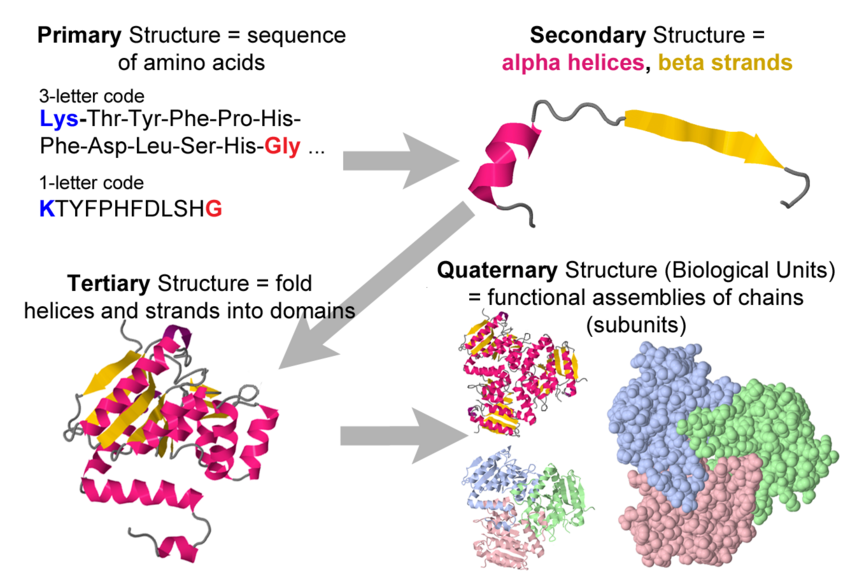
\includegraphics[width = 0.6\textwidth]{figs/850px-Protein-structure-4-levels-III-flat.png}
\caption{Los distintos niveles de la estructura proteica.}
\end{figure}

Es importante señalar que el enlace peptídico en sí no permite la rotación, ya que posee características parciales de doble enlace. Por lo tanto, la rotación está restringida a los enlaces entre el C$\alpha$ y el grupo C = O (el ángulo phi ($\phi$)) y el C$\alpha$ y el grupo NH (el ángulo psi ($\psi$)). Así pues, la cadena principal del polipéptido consiste en una secuencia repetida de dos enlaces giratorios seguidos de un enlace no giratorio (péptido). Sin embargo, no todos los 360º de los ángulos $\phi$ y $\psi$ son factibles debido a posibles \textbf{choques estéricos} entre cadenas laterales vecinas. Para determinados ángulos y combinaciones de aminoácidos, las restricciones espaciales impiden que los átomos ocupen la misma ubicación física, lo que explica en parte las distintas propensiones de ciertos aminoácidos a adoptar diferentes tipos de estructuras secundarias. 

\begin{figure}[h]
\centering
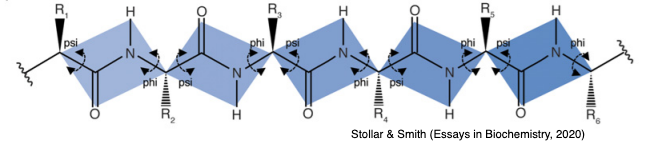
\includegraphics[width = 0.8\textwidth]{figs/peptide_bond.png}
\caption{Esquema de una cadena polipeptídica genérica. Las cadenas laterales de los residuos se denotan como R. Los rectángulos coloreados indican conjuntos de seis átomos que son coplanares debido al carácter de doble enlace del enlace peptídico. Las flechas indican los enlaces que son libres de rotar con el ángulo de rotación sobre el N-C$\alpha$ conocido como phi ($|phi$) y sobre el C$\alpha$-C conocido como psi ($\psi$). Obsérvese que sólo se etiquetan los enlaces del esqueleto peptídico y que, en la mayoría de los casos, el enlace del grupo R es libre de rotar.}
\end{figure}

Además, las cadenas laterales de los aminoácidos poseen sus propios ángulos de torsión, conocidos como $\chi1$, $\chi2$, $\chi3$, etc (figura \ref{fig:chi}). Estos ángulos de torsión influyen significativamente en las estructuras secundarias y, sobre todo, terciarias de las proteínas. Las distintas combinaciones de torsiones de las cadenas laterales definidas por los ángulos $\chi$ se denominan \textbf{rotámeros}.

\begin{figure}[h]
\centering
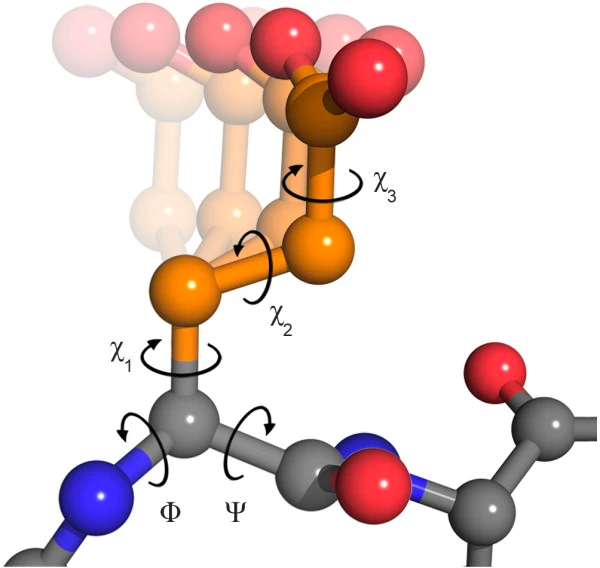
\includegraphics[width = 0.3\textwidth]{figs/paste-6EE800AE.png}
\caption{Ángulos diedros en el glutamato: Los ángulos diedros son los principales grados de libertad de la columna vertebral (ángulos $\phi$ y $\psi$) y la cadena lateral (ángulos $\chi$) de un aminoácido. El número de ángulos $\chi$ varía entre cero y cuatro para los 20 aminoácidos estándar. La figura muestra una representación esférica del glutamato, que tiene tres $\chi$ ángulos.}
\label{fig:chi}
\end{figure}

Dentro de estas limitaciones, las dos conformaciones locales primarias que evitan el impedimento estérico y maximizan el enlace de hidrógeno entre la columna vertebral y el backbone son las estructuras secundarias $\alpha$-hélice y $\beta$-hoja. Linus Pauling propuso inicialmente la hélice $\alpha$ como zurda en 1951, pero la estructura cristalina de la mioglobina en 1958 reveló que la forma diestra es más común. En las hélices diestras típicas, el grupo NH de la espina dorsal se une mediante enlaces de hidrógeno al grupo C=O de la espina dorsal del aminoácido situado cuatro residuos antes en la secuencia de la proteína. Esta forma de espiral regular tiene los grupos R apuntando hacia fuera, lejos de la espina dorsal peptídica, y requiere unos 3,6 residuos para completar una vuelta completa de la hélice (figura \ref{fig:alfa}).

\begin{figure}[h]
\centering
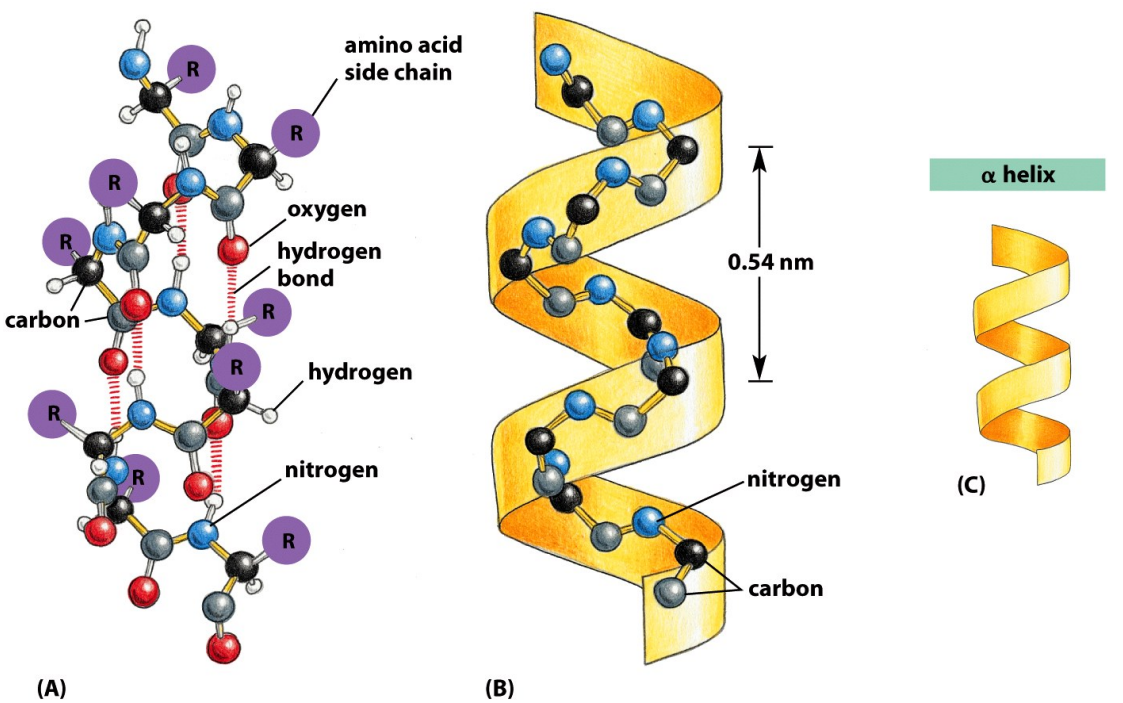
\includegraphics[width = 0.6\textwidth]{figs/alpha.png}
\caption{Hélice alfa.}
\label{fig:alfa}
\end{figure}

Las diferentes secuencias de aminoácidos tienen distintas tendencias a formar estructuras $\alpha$-helicoidales. La metionina, la alanina, la leucina, el glutamato y la lisina tienen propensiones especialmente altas a formar hélices, mientras que la prolina y la glicina tienen propensiones pobres a formar hélices. La prolina a menudo rompe o retuerce una hélice porque carece de un hidrógeno amida para formar enlaces de hidrógeno y su voluminosa cadena lateral interfiere con el esqueleto del giro precedente. La glicina, con sólo un hidrógeno como grupo R, es demasiado flexible y costosa desde el punto de vista entrópico para mantener la estructura $\alpha$-helicoidal, lo que la convierte en una rompedora de hélices $\alpha$.

\begin{figure}[h]
\centering
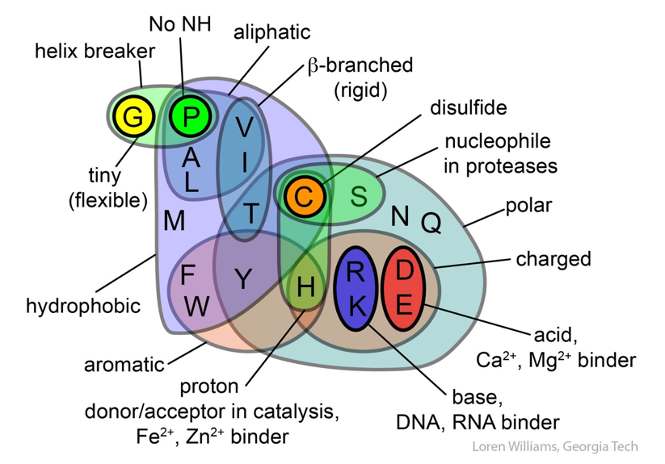
\includegraphics[width = 0.5\textwidth]{figs/aa.png}
\caption{Aminoácidos clasificados según su tipo.}
\end{figure}

Las láminas $\beta$ (figura \ref{fig:beta}) están formadas por dos o más cadenas polipeptídicas extendidas denominadas hebras $\beta$ que discurren una junto a otra en disposición paralela o antiparalela. En una lámina $\beta$, los residuos se disponen en zigzag y los enlaces peptídicos adyacentes apuntan en direcciones opuestas. El grupo NH y el grupo C=O de cada aminoácido forman enlaces de hidrógeno con el grupo C=O y el grupo NH, respectivamente, de las cadenas adyacentes. Las cadenas pueden ir en direcciones opuestas (lámina $\beta$ antiparalela) o en la misma dirección (lámina $\beta$ paralela). Las cadenas laterales de cada residuo se alternan en direcciones opuestas, dando a las láminas $\beta$ caras hidrofílicas e hidrofóbicas, formando a menudo un patrón de alternancia de residuos hidrofílicos e hidrofóbicos en la estructura primaria.

\begin{figure}[h]
\centering
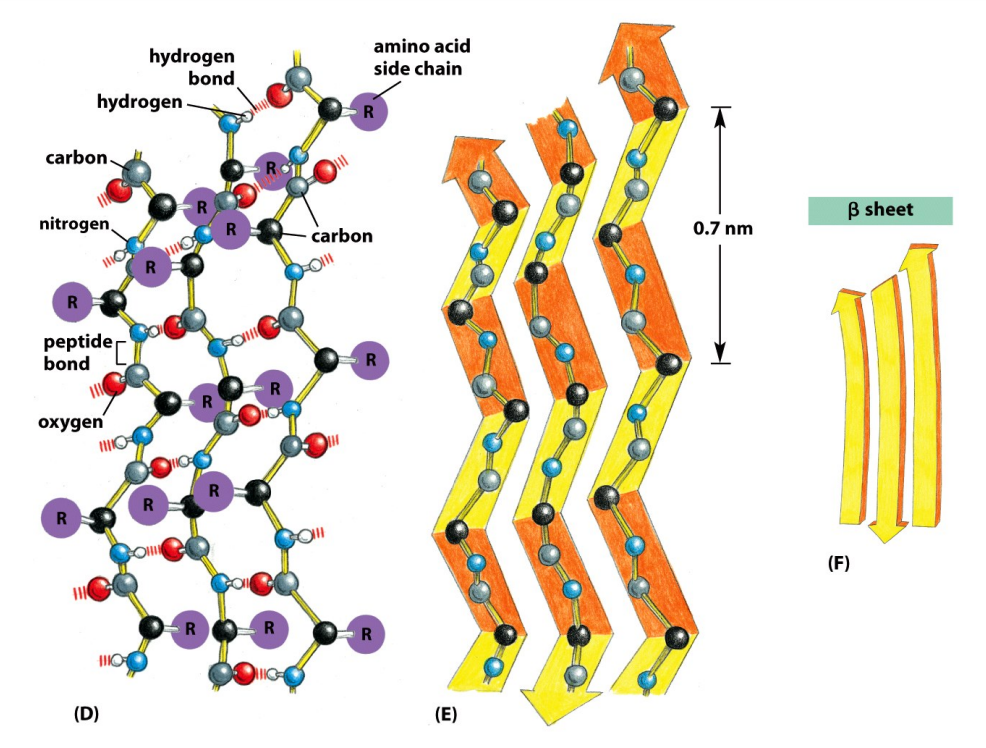
\includegraphics[width = 0.6\textwidth]{figs/beta.png}
\caption{Descripción detallada de una lámina beta formada por tres hebras beta.}
\label{fig:beta}
\end{figure}

Los residuos aromáticos grandes (tirosina, fenilalanina, triptófano) y los aminoácidos $\beta$-ramificados (treonina, valina, isoleucina) suelen encontrarse en las hebras $\beta$. Como en el caso de las hélices $\alpha$, las hebras $\beta$ suelen estar terminadas por glicinas, que son especialmente comunes en los giros $\beta$ (el conector más común entre hebras), como aminoácidos con ángulos $\phi$ positivos.

Las estructuras secundarias, terciarias y cuaternarias de las proteínas se mantienen gracias a las interacciones entre aminoácidos (figura \ref{fig:interactions}). Estas interacciones suelen clasificarse en cuatro tipos, que pueden ser tanto intra- como intermoleculares:
\begin{enumerate}
\item \textbf{Enlace iónico}: Los enlaces iónicos surgen de las atracciones electrostáticas entre cadenas laterales de aminoácidos cargadas positiva y negativamente. Por ejemplo, la atracción entre un ion carboxilato del ácido aspártico y un ion amonio de la lisina ayuda a estabilizar una región plegada específica de una proteína.
\item \textbf{Enlace de hidrógeno}: Los enlaces de hidrógeno se forman entre un átomo de oxígeno o nitrógeno altamente electronegativo y un átomo de hidrógeno unido a otro átomo de oxígeno o nitrógeno, como los de las cadenas laterales de aminoácidos polares. Los enlaces de hidrógeno son cruciales para las interacciones intra e intermoleculares en las proteínas, como en las hélices alfa.
\item \textbf{Enlaces disulfuro}. Cuando dos aminoácidos cisteína se acercan durante el plegamiento de la proteína en condiciones redox adecuadas, la oxidación puede unir sus átomos de azufre, formando un enlace disulfuro. A diferencia de los enlaces iónicos o de hidrógeno, se trata de enlaces covalentes, por lo que son un ejemplo clásico de reacción espontánea, que se produce como modificación postraduccional. Aunque son sensibles a los agentes reductores, estabilizan en gran medida la estructura terciaria y son vitales para la estructura cuaternaria de muchas proteínas, como los anticuerpos.
\item \textbf{Interacciones hidrofóbicas}. Las fuerzas de dispersión surgen cuando un átomo normalmente no polar se convierte momentáneamente en polar debido a una distribución desigual de electrones, dando lugar a un dipolo instantáneo que induce un desplazamiento de electrones en un átomo no polar vecino. Las fuerzas de dispersión son débiles, pero pueden ser importantes cuando otros tipos de interacciones no existen o son mínimas. El término interacción hidrofóbica suele utilizarse erróneamente como sinónimo de fuerzas de dispersión. Las interacciones hidrofóbicas surgen porque las moléculas de agua establecen enlaces de hidrógeno con otras moléculas de agua (o grupos de proteínas capaces de establecer enlaces de hidrógeno). Como los grupos no polares no pueden formar enlaces de hidrógeno, la proteína se pliega de tal forma que estos grupos quedan enterrados en la parte interior de la estructura proteica, minimizando su contacto con el agua.
\end{enumerate}

\begin{figure}[h]
\centering
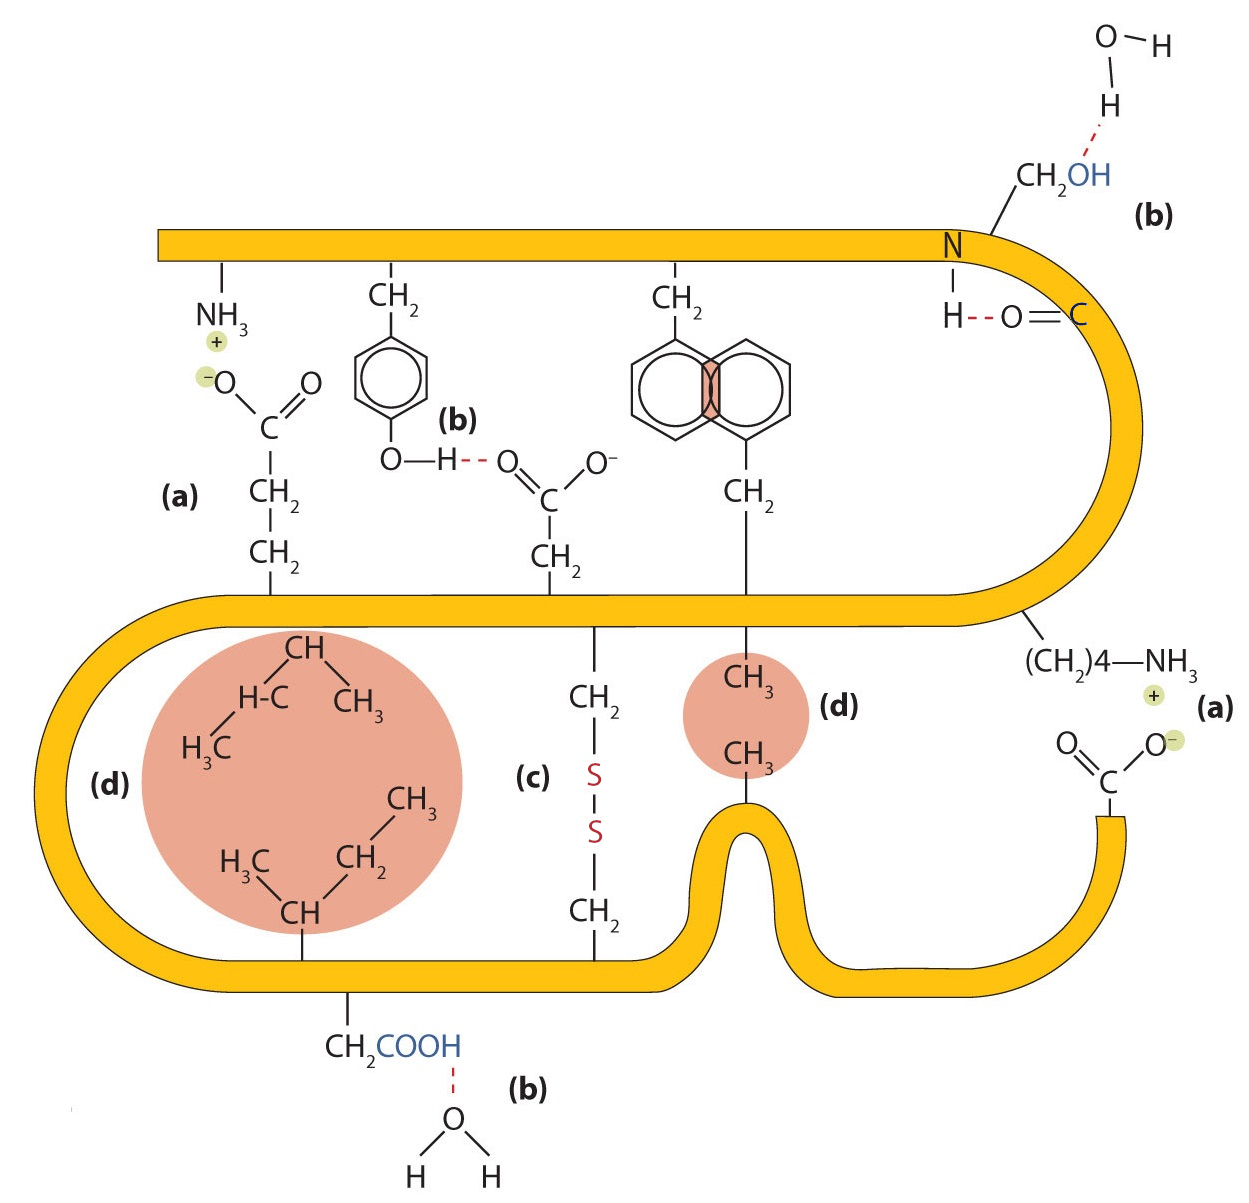
\includegraphics[width = 0.6\textwidth]{figs/interactions-01.png}
\caption{Cuatro interacciones estabilizan la estructura terciaria de una proteína: (a) enlace iónico, (b) enlace de hidrógeno, (c) enlaces disulfuro y (d) fuerzas de dispersión.}
\label{fig:interactions}
\end{figure}

Otras interacciones intramoleculares menos frecuentes podrían ser relevantes en algunas proteínas, como los llamados enlaces isopéptidos, formados entre dos grupos proteicos, al menos uno de los cuales no es un grupo $\alpha$-amino o $\alpha$-carboxi. Algunos ejemplos son la ubiquitilación, la sumoilación, la transglutaminación, el anclaje de proteínas a la superficie celular mediado por sortasas y la formación de pilus. Todos estos procesos comparten varias características (figura \ref{fig:iso}):
\begin{itemize}
\item Todos implican la reacción de un grupo $\epsilon$-amino de la lisina de una proteína con el grupo $\alpha$-carboxi principal de otra proteína, excepto en el caso de la transglutaminación, en la que la lisina se dirige a un grupo carboxiamida de la cadena lateral de la glutamina.
\item Todos los procesos están mediados por enzimas e implican un intermediario tioéster transitorio formado por la cisteína del sitio activo. Este intermediario se resuelve mediante un ataque nucleofílico por el grupo $\epsilon$-amino de la lisina, que completa la formación del enlace.
\end{itemize}

\begin{figure}[h]
\centering
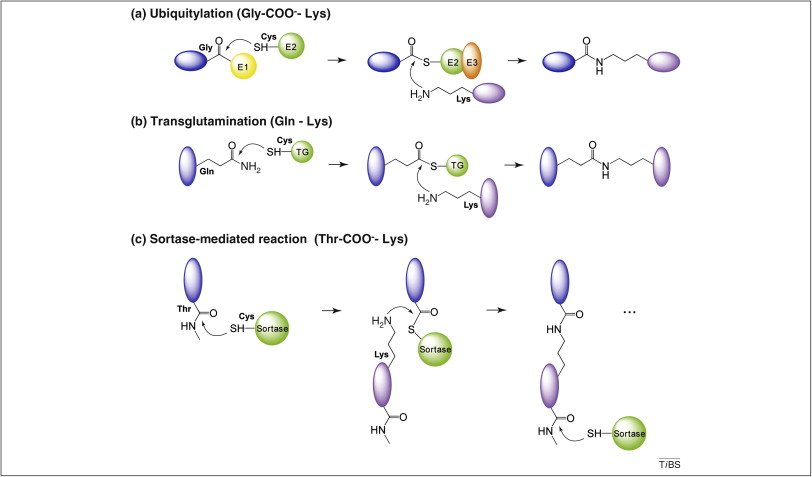
\includegraphics[width = 0.8\textwidth]{figs/iso.jpg}
\caption{Formación de enlaces isopeptídicos intermoleculares mediada por enzimas. Se muestran ejemplos de tres procesos biológicos diferentes: ubiquitilación, transglutaminación y ensamblaje de pilus mediado por sortasa en bacterias Gram positivas. Las proteínas unidas por enlaces isopeptídicos están coloreadas en azul y morado y las enzimas formadoras de enlaces isopeptídicos en verde.}
\label{fig:iso}
\end{figure}

A diferencia de estos procesos dependientes de enzimas, los enlaces isopeptídicos entrecruzados (intrachain isopeptide bonds) se forman autocatalíticamente en la pilina principal Spy0128 de \textit{S. pyogenes} y en otras proteínas de la superficie de células Gram+, así como en la cápside del fago HK97. En este caso, la reacción de formación del enlace es una reacción inducida por la proximidad que se produce cuando los aminoácidos participantes se sitúan juntos en un entorno hidrofóbico, ya sea a través del plegamiento de la proteína concurrente con la formación del enlace peptídico en el ribosoma o por la reorganización de la cápside (en HK97).

En cuanto a la ingeniería proteica, es posible crear aminoácidos no naturales reactivos. Esto se ha utilizado para aumentar la termoestabilidad de proteínas como anticuerpos, crear recombinantes y unir covalentemente proteínas a superficies o nanopartículas.

\subsection{Gráfico de Ramachandran}
Muchas combinaciones de ángulos $\phi$ y $\psi$ están prohibidas debido al principio de exclusión estérica, que dicta que dos átomos no pueden ocupar el mismo espacio simultáneamente. Este concepto fue demostrado inicialmente por Gopalasamudram Ramachandran, que desarrolló un gráfico para visualizar los valores de ángulo permitidos, conocido como gráfico de Ramachandran. Este gráfico puede mostrar los ángulos de un aminoácido específico, de todos los aminoácidos de una proteína o incluso de muchas proteínas. El análisis de los ángulos $\phi$ y $\psi$ en proteínas conocidas revela que aproximadamente tres cuartas partes de todas las combinaciones posibles de $\phi$, $\psi$ no están permitidas (figura \ref{fig:ramachandran}) y se corresponden con motivos comunes de estructura secundaria (figura \ref{fig:ramachandran2}).

\begin{figure}[h]
\centering
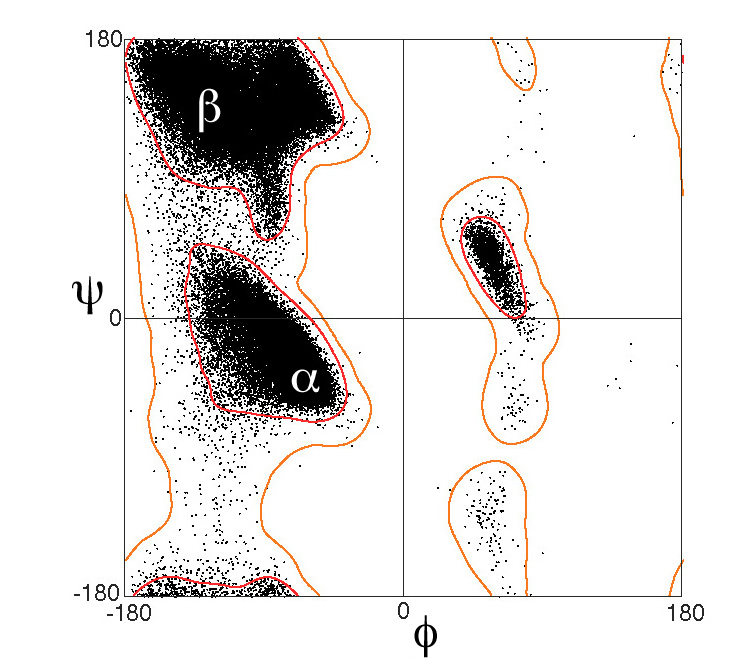
\includegraphics[width = 0.6\textwidth]{figs/Ramachandran_plot_general_100K.jpg}
\caption{Diagrama general de Ramachandran. La densidad de puntos refleja la probabilidad de cada combinación de ángulos, definiendo las regiones central (línea roja) y de tolerancia (naranja).}
\label{fig:ramachandran}
\end{figure}

\begin{figure}[h]
\centering
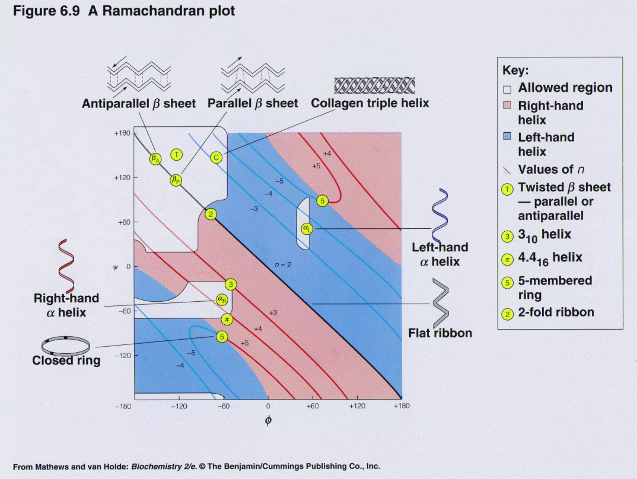
\includegraphics[width = 0.6\textwidth]{figs/rama2.png}
\caption{Definición de alternativas de estructura secundaria por su combinación de ángulos phi, psi.}
\label{fig:ramachandran2}
\end{figure}

Los residuos funcionalmente relevantes son más propensos que otros a tener ángulos de torsión que se sitúan en las regiones permitidas pero desfavorecidas de un diagrama de Ramachandran. La geometría específica de estos residuos relevantes desde el punto de vista funcional, aunque desfavorable desde el punto de vista energético, puede ser importante para la función de la proteína, ya sea catalítica o de otro tipo. Tales conformaciones deben ser estabilizadas por la proteína mediante enlaces H, empaquetamiento estérico u otros medios, y rara vez se dan en residuos muy expuestos a disolventes.

Suele haber espacios designados para las hélices $\alpha$ y las láminas $\beta$, pero también puede haber outliers que muestren aminoácidos concretos.

\subsection{Pliegues (folds), dominios y motivos de proteínas}
La estructura terciaria tridimensional global de una proteína se conoce comúnmente como su \textbf{pliegue}, definiendo así la forma y orientación global ignorando los loops. Dentro del pliegue proteico global, podemos reconocer distintos dominios y motivos. Los \textbf{dominios} son secciones compactas de la proteína que representan regiones estructural y (normalmente) funcionalmente independientes. Eso significa que un dominio mantiene sus características principales, aunque se separe de la proteína global. Por otro lado, los \textbf{motivos} son pequeñas subestructuras que no son necesariamente independientes y que constan sólo de unos pocos tramos de estructura secundaria. De hecho, los motivos también pueden denominarse superestructuras secundarias y son frecuentes en la secuencia. En resumen, un dominio corresponde a un fold, y una cadena peptídica puede tener uno o varios dominios.

La diversidad de pliegues, dominios y motivos proteicos, así como su combinación, puede utilizarse para clasificar jerárquicamente las estructuras proteicas, como en muchos otros campos de la biología. La primera clasificación se propuso en los años 70 y consistía en cuatro grupos de pliegues, como se muestra en la siguiente figura. Todas las proteínas $\alpha$ se basan casi por completo en una estructura $\alpha$-hélice, y todas las estructuras $\beta$ se basan en $\beta$-láminas. La estructura $\alpha$/$\beta$ se basa en una mezcla de $\alpha$-hélices y $\beta$-láminas, a menudo organizadas como $\beta$-hebras paralelas conectadas por $\alpha$-hélices. Por otro lado, las estructuras $\alpha$+$\beta$ consisten en motivos discretos de $\alpha$-hélice y $\beta$-lámina que no están entrelazados (como ocurre en las proteínas $\alpha$/$\beta$). Por último, las proteínas pequeñas abarcan polipéptidos con estructuras secundarias nulas o escasas.

\begin{figure}[h]
\centering
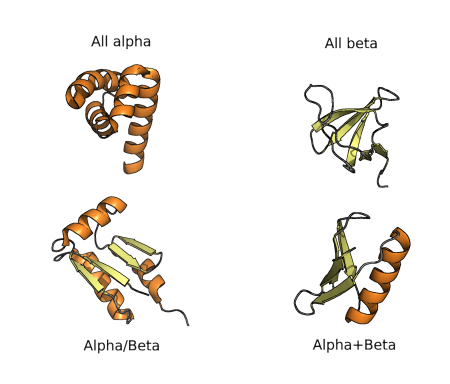
\includegraphics[width = 0.6\textwidth]{figs/clasif.png}
\caption{Las cuatro clases de proteínas estructurales de la clasificación de Chlothia y Levitt.}
\label{fig:alphabeta}
\end{figure}
%31/01 - Modesto
\chapter{Bases de datos de proteínas}
\section{Comparación de estructura y alineamiento}
Para comprender la diversidad y función de las proteínas, es importante comparar sus secuencias y estructuras. Esto ayuda a encontrar patrones comunes y a comprender su diversidad e historia evolutiva. Midiendo y analizando estas similitudes, los científicos pueden clasificar las proteínas y determinar sus relaciones en términos de función y evolución. Este proceso también es crucial en el modelado de proteínas, ya que ayuda a identificar, evaluar y elegir modelos intermedios.

Es esencial aclarar la distinción entre alineamiento y superposición, ya que estos términos se confunden con frecuencia en la literatura. Un \textbf{alineamiento estructural} pretende identificar similitudes y diferencias entre dos estructuras, mientras que la \textbf{superposición de estructuras} muestra las estructuras basándose en criterios específicos, normalmente derivados de un alineamiento estructural previo. Por consiguiente, la superposición trata de minimizar la distancia entre estructuras identificando una transformación que consiga la menor desviación cuadrática media (RMSD) o las máximas equivalencias dentro de un límite RMSD.

La RMSD puede calcularse para cualquier par de moléculas. En el contexto de las proteínas, solemos referirnos a la RMSD de los alfa-carbones. Una alineación superior facilitará una mejor superposición. Por lo tanto, aunque la alineación y la superposición son procesos distintos, la RMSD puede servir como indicador de ambos; cuanto menor sea la RMSD, mejor será la alineación/superposición. Es importante señalar que la RMSD es una medida de distancia real, no una puntuación. Eso implica que sólo podemos obtener la RMSD para los residuos alineados, no para toda la secuencia de cualquiera de las dos proteínas. Por lo tanto, una RMSD de 1 $\AA$ puede indicar una distancia cercana pero, si implica a muy pocos aminoácidos, no sugiere necesariamente una buena similitud. Tanto el valor RMSD como el número de residuos alineados deben tenerse en cuenta para un análisis preciso.

\begin{figure}[h]
\centering
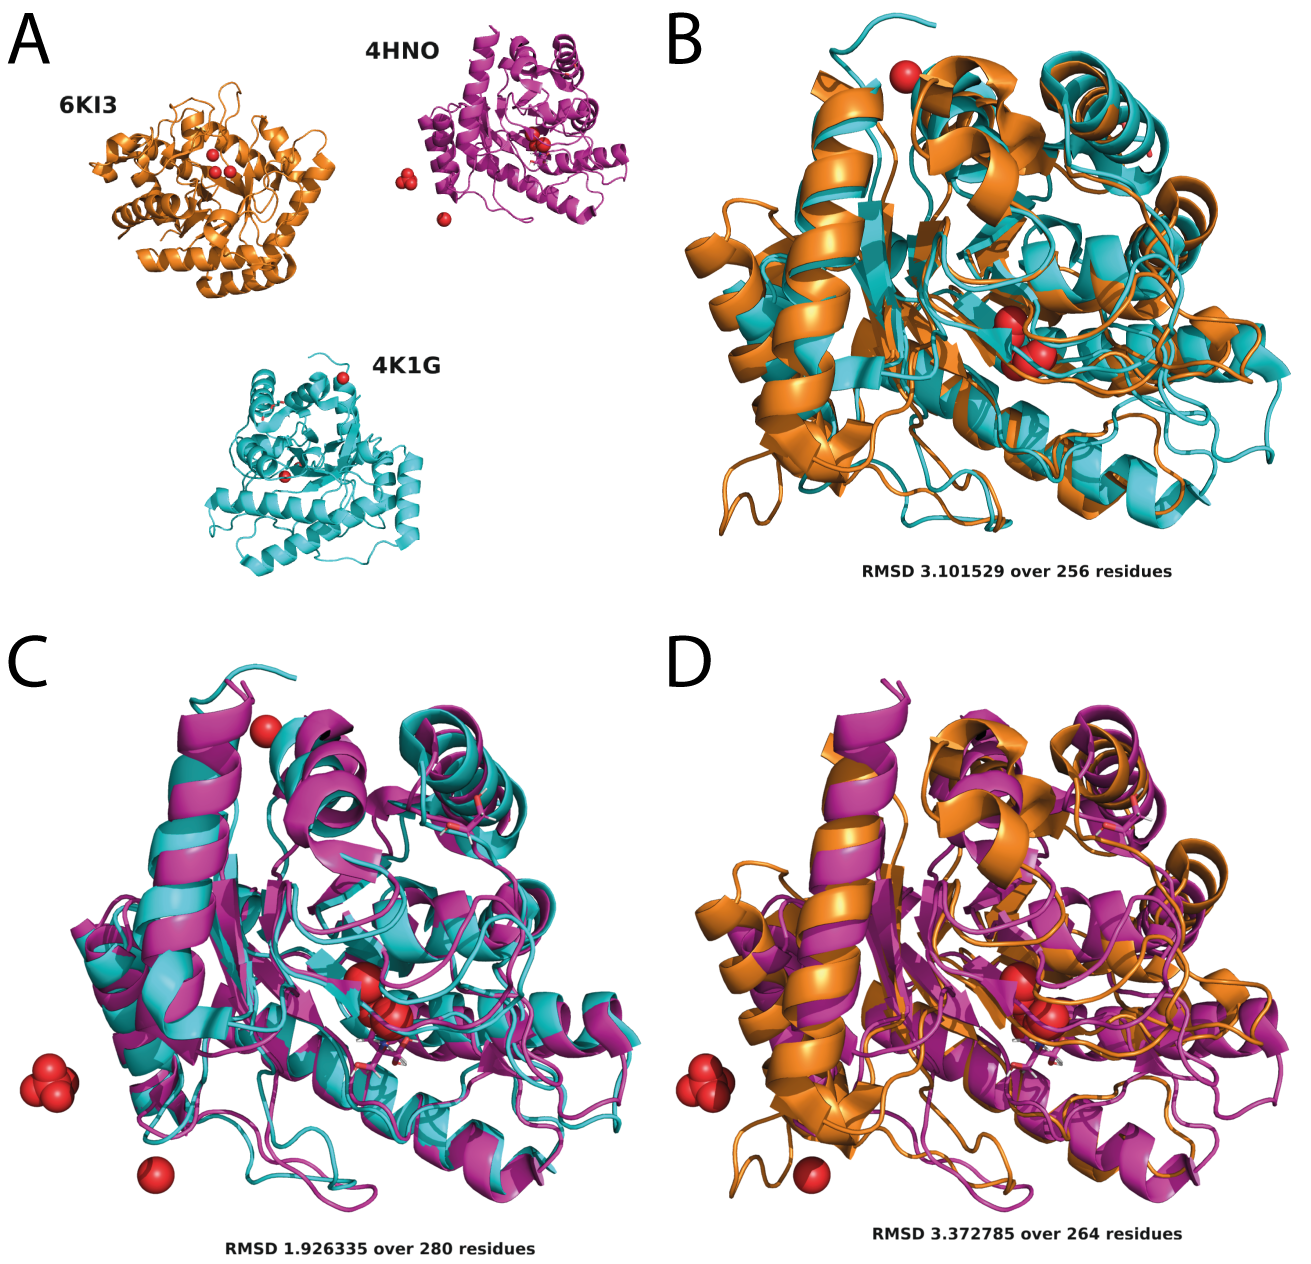
\includegraphics[width = 0.6\textwidth]{figs/rmsd.png}
\end{figure}

Global Distance Test se utiliza en CASP al ser menos sensible a outliers y permite comparar estructuras de secuencias idénticas. Se normaliza el número de residuos que caigan bajo un límite.

\section{Principales bases de datos de proteínas}
La clasificación de secuencias proteicas nos ayuda a comprender la diversidad de las distintas proteínas mediante el examen de sus secuencias, lo que se conoce como el \textbf{espacio de secuencias proteicas} (el concepto matemático de espacio). Por otro lado, la clasificación de las estructuras proteicas consiste en agrupar las proteínas en función de sus relaciones estructurales. Algunas clasificaciones tienen en cuenta la vecindad estructural (continuo estructural), mientras que otras utilizan el concepto de evolución de las proteínas como principal factor de diversificación, lo que da lugar a un \textbf{espacio de estructuras proteicas} discreto en lugar de continuo.

Esta sección no pretende ofrecer una revisión exhaustiva de todas las bases de datos de proteínas. En consecuencia, no cubriremos en detalle la base de datos de proteínas del NCBI, que se utiliza ampliamente para diversos fines y probablemente se mencione en otros cursos. La Base de Datos de Proteínas del NCBI sirve principalmente como repositorio principal de secuencias, con un énfasis mínimo en el análisis de la diversidad y clasificación de proteínas. Esta sección destacará las principales diferencias y aplicaciones de Pfam, Uniprot, Prosite, PDB, SCOP y CATH. 

\begin{figure}[h]
\centering
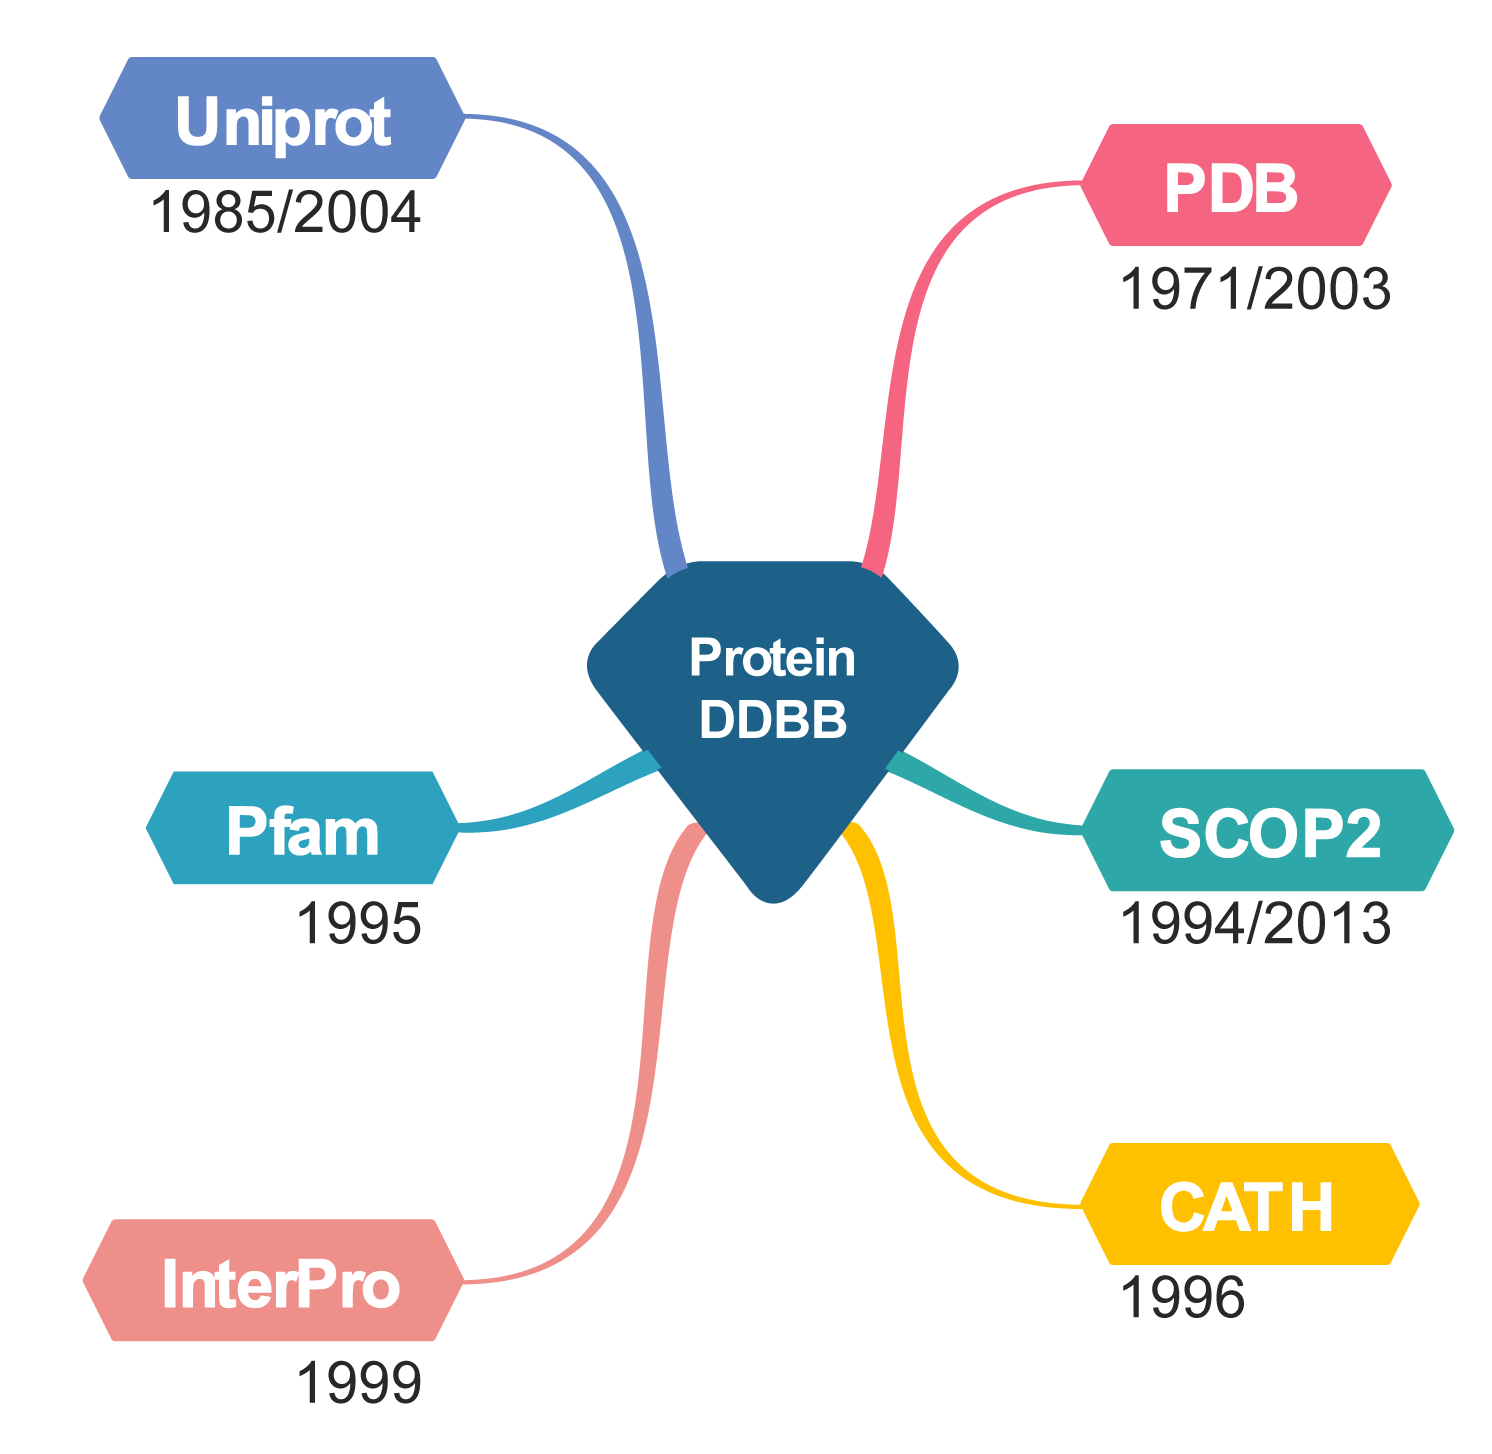
\includegraphics[width = 0.4\textwidth]{figs/ddbb.png}
\end{figure}

En bioinformática, las bases de datos suelen clasificarse en primarias o secundarias. Las \textbf{bases de datos primarias} contienen datos obtenidos experimentalmente, como secuencias de nucleótidos, secuencias de proteínas o estructuras macromoleculares. Es importante señalar que, una vez asignado el número de acceso a una base de datos, los datos de las bases de datos primarias permanecen inalterados y forman parte del registro científico. En cambio, las \textbf{bases de datos secundarias} incluyen datos derivados del análisis de datos primarios. Estas bases de datos suelen utilizar información procedente de numerosas fuentes, incluidas otras bases de datos y la literatura científica. Suelen ser muy complejas e implican una compleja combinación de algoritmos informáticos y/o análisis e interpretación manuales para generar nuevos conocimientos a partir del registro público de la ciencia.

Aunque la distinción entre bases de datos primarias y secundarias se ha vuelto menos clara en los últimos tiempos debido a la integración de datos procedentes de diversas fuentes, aún pueden distinguirse algunas diferencias. Las principales bases de datos primarias para secuencias de proteínas son NCBI Protein y RCSB-PDB para estructuras proteicas. UniProt también alberga una base de datos primaria de secuencias denominada TrEMBL y, desde 2002, incorpora la base de datos PIR-PSD, que reúne los recursos de Protein Information Resource, EMBL y SIB en una única metabase de datos (véase PIR-PSD). Por otra parte, RCSB-PDB es la principal base de datos estructural primaria, mientras que SCOP2 y CATH son bases de datos secundarias notables.

\begin{figure}[h]
\centering
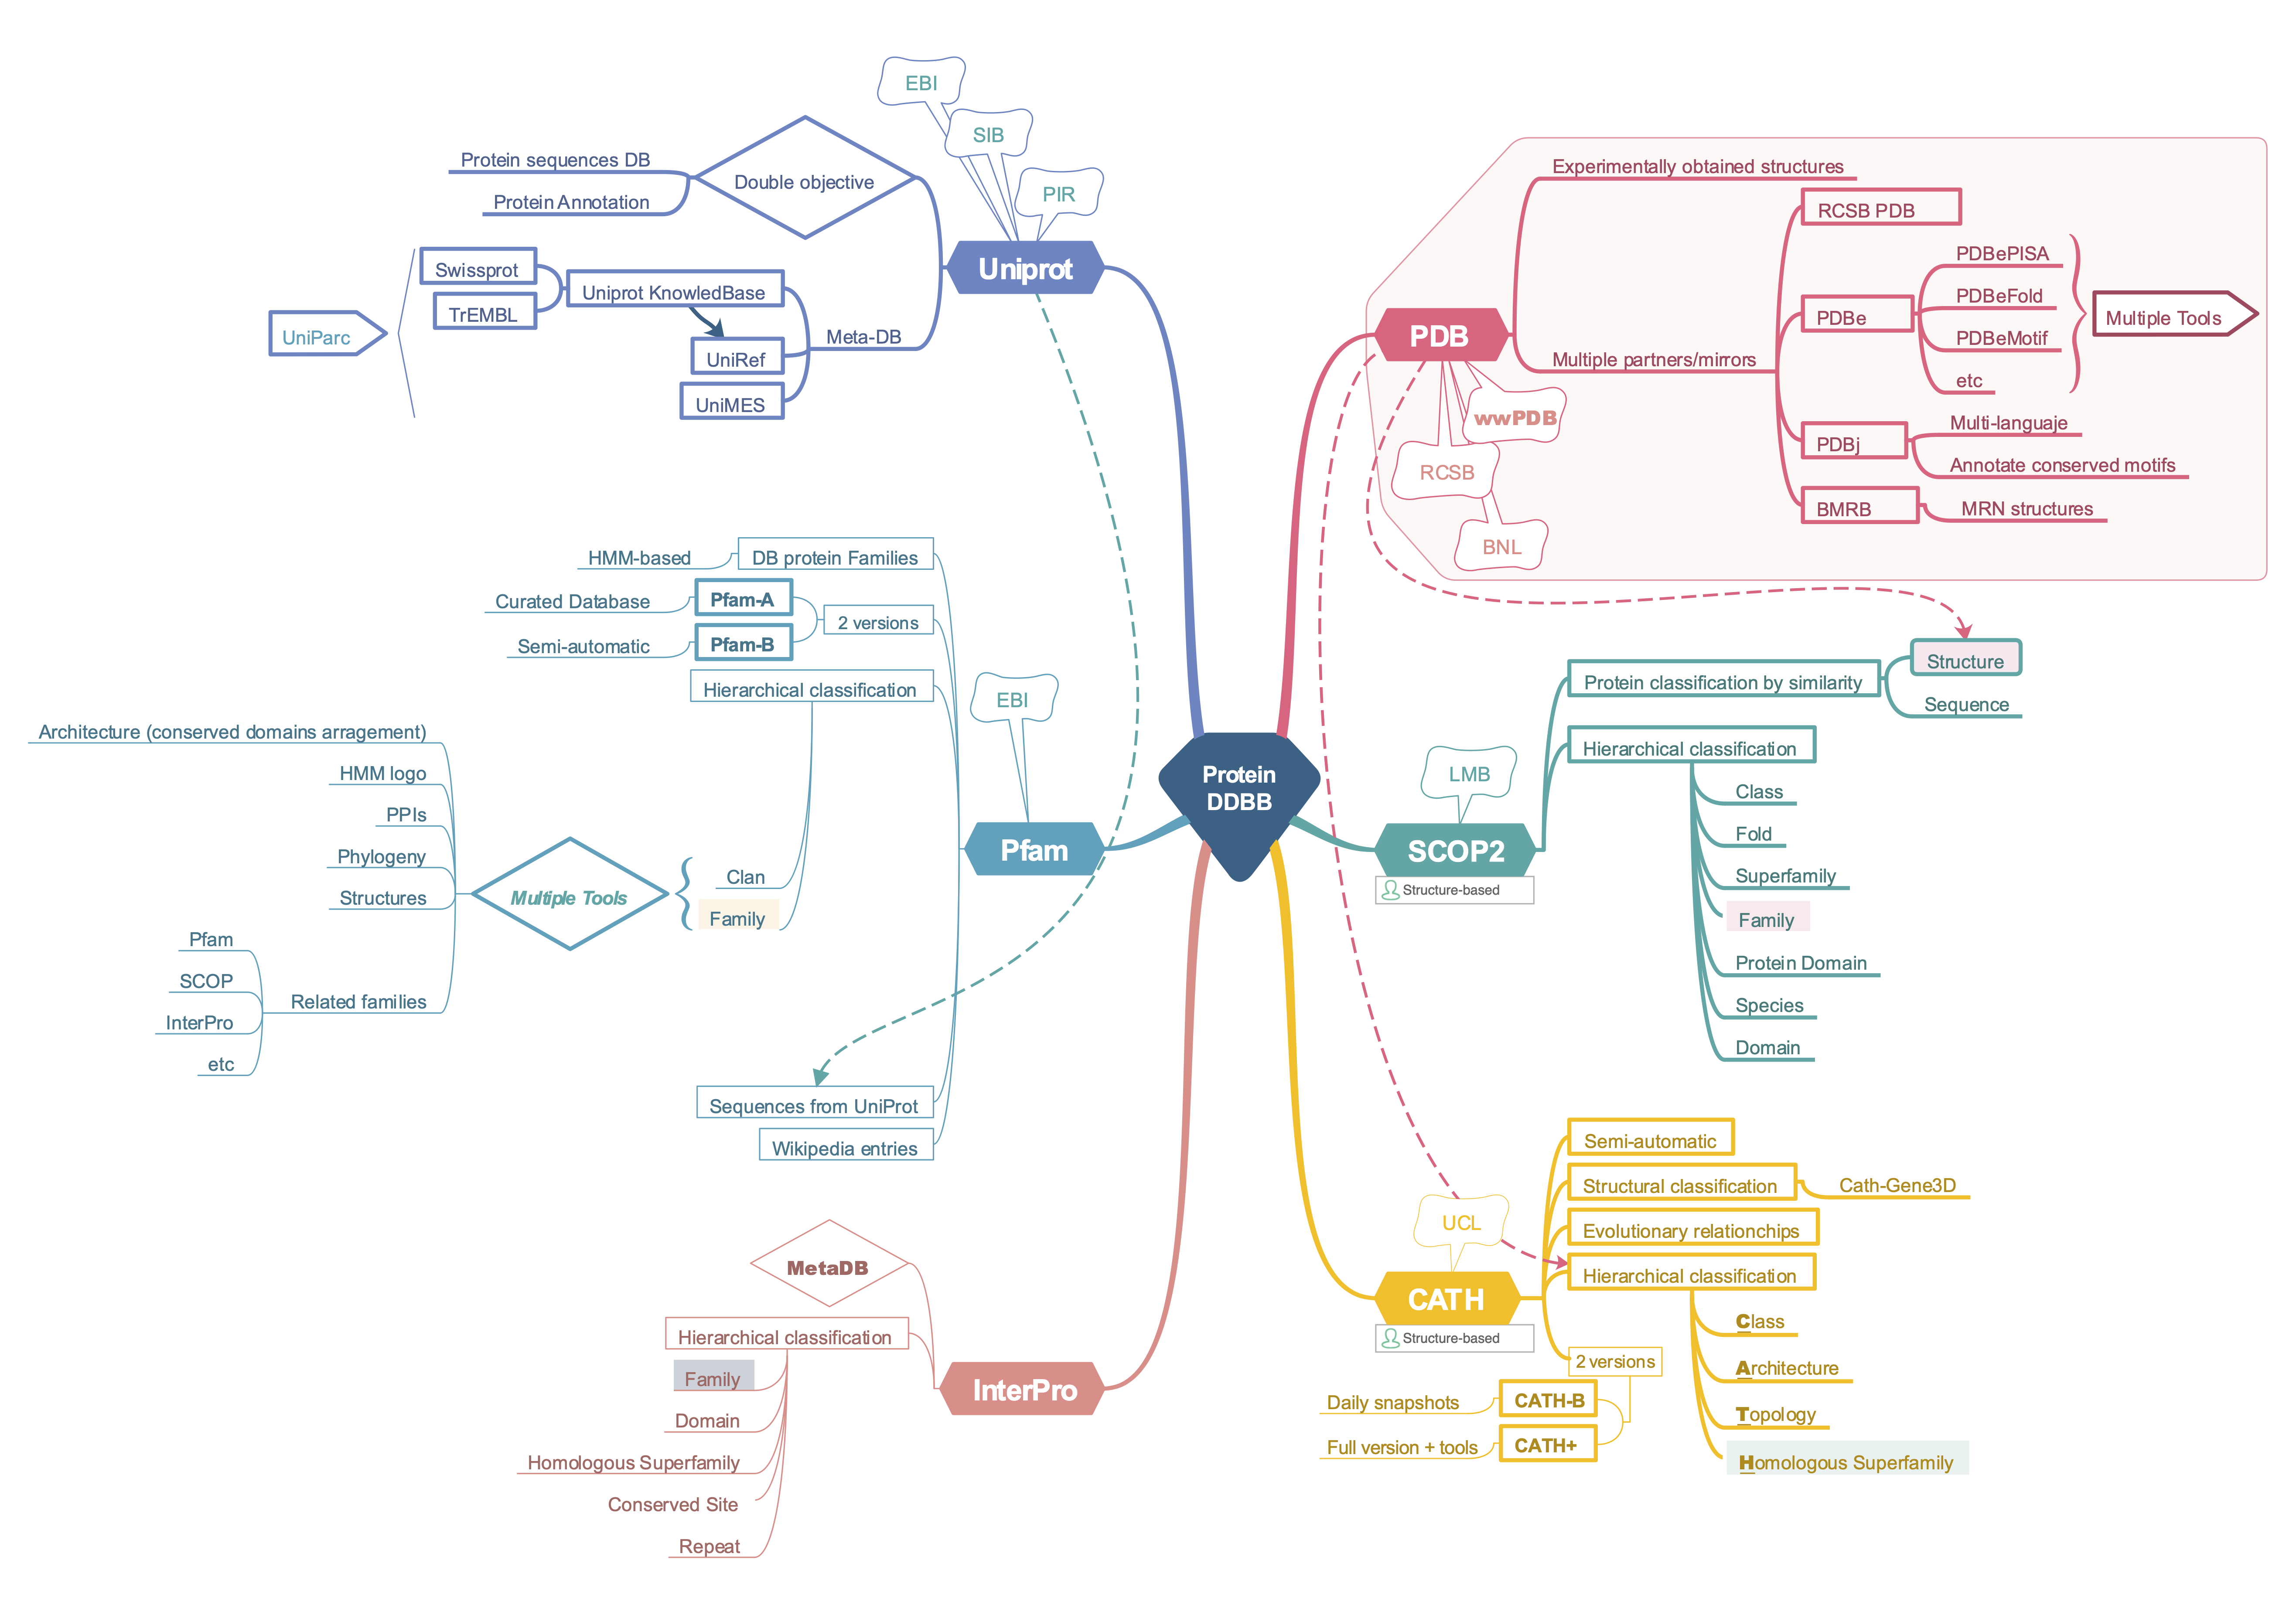
\includegraphics[width = 0.9\textwidth]{figs/bbdd_full.png}
\end{figure}

\begin{table}[htbp]
\begin{mdframed}[backgroundcolor=black!10]
    \centering
    Todas las bases de datos que describimos aquí permiten el acceso mediante programación y/o API, normalmente con paquetes BioPython y R, lo que aumenta significativamente las posibilidades de programación y análisis de datos por lotes.
    \end{mdframed}
\end{table}

\subsection{Bases de datos estructurales}
\subsubsection{RCSB-PDB}
La base de datos Protein Data Bank es la principal base de datos estructural primaria de macromoléculas. Contiene principalmente estructuras de proteínas, pero también abarca ácidos nucleicos y complejos nucleoproteicos. PDB cumplió 50 años en 2021 y se puede ver un resumen detallado de su historia en el sitio RCSB-PDB.

Brevemente, el PDB se creó en 1971 en el Laboratorio Nacional de Brookhaven con sólo 7 estructuras. Posteriormente, el \textbf{Research Collaboratory for Structural Bioinformatics (RCSB)}, formado por Rutgers, UCSD/SDSC y CARB/NIST, se hizo responsable de la gestión del PDB en 1998 en respuesta a una RFP y un largo proceso de revisión. En 2003, se creó el Worldwide Protein Data Bank (wwPDB) para mantener un único archivo PDB de datos estructurales macromoleculares a disposición libre y pública de la comunidad mundial. Está formado por organizaciones que actúan como centros de depósito, procesamiento y distribución de datos PDB.

Las estructuras del PDB se obtienen en gran medida mediante cristalografía de rayos X, pero acepta derivaciones de datos de EM y RMN desde 1989 y 1991, respectivamente. De hecho, el BMRB (Biological Magnetic Resonance Bank) se ha asociado con el PDB desde 2006 y el EMBD (Electron Microscopy Data Bank) desde 2021. Además, a partir de septiembre de 2022, el PDB también contiene modelos computados de la base de datos Alphafold (de la que hablaremos más adelante en este curso) y RoseTTAFold-ModelArchive. \textbf{Así pues, la base de datos PDB es el eje principal que centraliza las estructuras biológicas en la actualidad}.

La base de datos PDB tiene cuatro réplicas y sitios web (RCSB, Europa, BMRB y Japón) con información que se solapa principalmente, aunque tienen cierta especialización. El sitio PDB del RCSB tiene también una sección educativa (PDB-101) con información y recursos muy útiles para la enseñanza y el aprendizaje de la biología estructural y el trabajo con estructuras PDB.

%PREGUNTA EXAMEN: Verdadero o falso, PDB tiene estructuras computacionales

Las entradas del PDB contienen toda la información sobre la estructura, desde la secuencia de la proteína y su origen hasta los detalles del experimento, así como la evaluación de la estructura y la visualización. Se puede descargar toda esta información y las coordenadas de la estructura en diversos formatos de archivo.

\subsubsection{SCOP}
La base de datos Structural Classification of Proteins (SCOP, http://scop.mrc-lmb.cam.ac.uk) es una \textbf{clasificación de dominios proteicos} organizada según sus relaciones evolutivas y estructurales en categorías jerárquicas. La unidad principal es la \textbf{familia}, que agrupa proteínas relacionadas con pruebas claras de su origen evolutivo, mientras que la \textbf{superfamilia} reúne dominios proteicos relacionados de forma más distante. Además, las superfamilias se agrupan en \textbf{pliegues} distintos en función de las características estructurales globales que comparten la mayoría de sus miembros. Se proporcionan definiciones de dominio para los dos niveles principales de la clasificación SCOP, familia y superfamilia, y los límites de dominio para cada uno de ellos pueden coincidir o diferir.

Para cada grupo, se selecciona un representante basándose en su secuencia (UniProtKB) y estructura (PDB) y se utiliza para la clasificación SCOP. Así, los límites de dominio SCOP se asignan tanto a la entrada PDB como a la UniProtKB.

\subsubsection{CATH}
CATH (www.cathdb.info) es un recurso gratuito y de acceso público que identifica dominios proteicos dentro de proteínas del Banco de Datos de Proteínas y los clasifica en grupos relacionados evolutivamente según la información sobre secuencia, estructura y función. Parte de la base de que las proteínas relacionadas que se pliegan de forma similar suelen exhibir funciones similares (esto sólo podría demostrarse si encontramos intermediarios). CATH utiliza un esquema de clasificación jerárquica en el que las unidades comparadas y clasificadas son dominios estructurales. Los dominios, definidos aquí como dominios estructurales globulares capaces de plegarse de forma semiindependiente, se extraen de estructuras de proteínas determinadas experimentalmente y disponibles en la base de datos PDB. Los dominios se clasifican en los siguientes niveles jerárquicos que componen el nombre CATH: Clase (C), Arquitectura (A), Topología (T) y Superfamilias homólogas (H).

CATH utiliza una combinación de varios algoritmos basados en estructuras (SSAP, CATHEDRAL) y en secuencias (alineaciones de secuencias basadas en Needleman-Wunsch, Jackhmmer, Profile Comparer y HHsearch) para evaluar la similitud de los dominios entre sí e identificar proteínas homólogas.

CATH tiene un recurso hermano, Gene3D, que añade secuencias adicionales de dominios de proteínas sin estructura conocida, lo que eleva el número total actual de dominios en CATH-Gene3D a 95 millones.

La base de datos CATH se actualiza con bastante regularidad mediante instantáneas diarias (CATH-B), pero cada 12 meses se publica una versión completa con más herramientas, denominada CATH+. CATH-plus contiene familias funcionales (CATH-FunFams), clusters estructurales y otras herramientas.

\subsection{Bases de datos de secuencias}
\subsubsection{Uniprot}
Las bases de datos Uniprot están gestionadas por el consorcio UniProt, creado en 2002 por EMBL-EBI, SIB y PIR. En la actualidad, UniProt puede considerarse una metadatabase, ya que sus entradas contienen información procedente de diversas fuentes. Se creó con dos objetivos principales: establecer una base de datos de secuencias de proteínas completa y no redundante y enriquecer esa base de datos con anotaciones detalladas. Estas anotaciones incluyen familias de proteínas y genes, datos de función y estructura-función, interacciones con otras proteínas o cofactores, localización, patrones de expresión, variantes, etc. Así, pretende cumplir los objetivos tanto de las bases de datos primarias como de las secundarias.

El eje central de las bases de datos UniProt es la Uniprot Knowledgebase. Se trata de una colección de información funcional sobre proteínas, con anotaciones precisas, coherentes y ricas. UniProtKB consta de dos bases de datos internas: una sección contiene registros anotados manualmente con información extraída de la bibliografía, sugerencias de la comunidad y análisis computacionales revisados por los conservadores. La otra sección incluye registros analizados computacionalmente. Estas secciones se denominan «UniProtKB/Swiss-Prot» (revisada, anotada manualmente) y «UniProtKB/TrEMBL» (no revisada, anotada automáticamente), respectivamente.
En los últimos años, UniProtKB ha incorporado datos estructurales de la base de datos Alphafold, además de referencias cruzadas a información estructural. 

UniProt contiene secuencias con distintos niveles de detalle de anotación en dos bases de datos complementarias: Uniparc y Uniref. En resumen, UniParc (UniProt Archive) es una base de datos exhaustiva y no redundante que incluye la mayoría de las secuencias de proteínas disponibles públicamente en todo el mundo. UniParc evita la redundancia almacenando cada secuencia única una sola vez y asignándole un identificador único estable (UPI), que permite identificar la misma proteína a partir de diferentes bases de datos fuente. Un UPI nunca se elimina, cambia o reasigna. Por otro lado, UniRef (UniProt Reference Clusters) proporciona conjuntos agrupados de secuencias de UniProtKB (y registros seleccionados de UniParc) para garantizar una cobertura completa del espacio de secuencias a varias resoluciones, ocultando al mismo tiempo las secuencias redundantes (pero no sus descripciones). 
La base de datos UniRef100 combina secuencias idénticas en una única entrada UniRef, mostrando la secuencia de una proteína representativa, los números de acceso de todas las entradas fusionadas y enlaces a las bases de datos correspondientes. UniRef90 se construye agrupando secuencias UniRef100 utilizando el algoritmo MMseqs2, de modo que cada clúster consiste en secuencias con al menos un 90\% de identidad de secuencia y un 80\% de solapamiento con la secuencia más larga (la secuencia semilla ) del clúster. Del mismo modo, UniRef50 se construye agrupando secuencias semilla UniRef90 que tienen al menos un 50\% de identidad de secuencia y un 80\% de solapamiento con la secuencia más larga del clúster. UniParc y UniRef sólo contienen secuencias de proteínas; el resto de la información sobre las proteínas debe recuperarse de las bases de datos de origen utilizando referencias cruzadas de bases de datos.

\subsubsection{InterPro}
InterPro pretende ser una base de datos funcional secundaria, clasificando las proteínas en familias, dominios y sitios importantes. Para clasificar las proteínas de este modo, InterPro utiliza modelos predictivos, conocidos como firmas, proporcionados por varias bases de datos diferentes (hasta 13) que conforman el consorcio InterPro. InterPro combina esas diferentes firmas que representan familias, dominios o sitios equivalentes, y proporciona información adicional como descripciones, referencias bibliográficas y términos de la Ontología Genética (GO), para producir un recurso completo para la clasificación de proteínas.

La base de datos InterPro se actualiza cada 2 meses y es muy útil para la anotación de ORFans o proteínas divergentes. En los últimos años, ha integrado más recursos, incluyendo Pfam, así como datos estructurales y predicciones, dando lugar a un recurso muy práctico para múltiples propósitos en la ciencia de las proteínas.

Interpro se creó como una BBDD de secuencias, pero actualmente se encuentra en un punto intermedio. Ahora se podría decir que es más bien una «metabase de datos» que contiene información sobre secuencias y estructuras.

\subsubsection{Pfam}
Pfam es una base de datos de proteínas cuyo objetivo es clasificar secuencias por sus relaciones evolutivas. Se fundó en 1995 y ha sido muy útil para la anotación funcional de datos genómicos. El sitio web de Pfam (http://pfam.xfam.org/) se cerró a finales de 2022. Sin embargo, la base de datos Pfam no se interrumpió, sino que se integró en el sitio InterPro. Pfam utiliza perfiles HMM para clasificar las proteínas en familias, que se agrupan en clanes. 

La versión actual (37.1) contiene 23.794 entradas y 751 clanes. Pfam se diseñó como una base de datos que debe actualizarse con frecuencia en la era genómica de avance rápido. Para ello, utiliza dos tipos de alineación. Cada familia Pfam tiene un alineamiento semilla que contiene un conjunto representativo de secuencias para la entrada. A partir del alineamiento semilla se construye automáticamente un modelo de Markov oculto (HMM) de perfil y se busca en una base de datos de secuencias denominada pfamseq utilizando el software HMMER3 (http://hmmer.org/). Todas las regiones de secuencias que satisfacen un umbral curado específico de la familia, también conocido como umbral de reunión, se alinean con el HMM de perfil para crear el alineamiento completo.

Además de las entradas Pfam basadas en HMM (Pfam-A), los perfiles Pfam se utilizan para proporcionar un conjunto de alineaciones de secuencias múltiples no anotadas, generadas computacionalmente, denominadas Pfam-B. Sin embargo, en las últimas versiones de Pfam, los alineamientos Pfam-B sólo se publican actualmente en el sitio FTP de Pfam.

Pfam también se ha utilizado en la creación de otros recursos como Rfam (familias de ARN) y Dfam (elementos transponibles de ADN).

\section{Estrategias actuales y futuras en las bases de datos de proteínas}
Existe una tendencia significativa hacia el cruce y la integración de datos diversos dentro de las \textbf{metadatabases}. Un caso ejemplar es el Human Protein Atlas, que proporciona información sobre proteínas clasificadas por tipo celular o tejido, junto con detalles sobre variantes de splicing, mutantes, etc. Además, es importante reconocer las nuevas bases de datos estructurales, como la base de datos Alphafold de Deepmind y el Atlas Metagenómico ESM, que albergan millones de estructuras de proteínas predichas mediante métodos de aprendizaje profundo. También existen bases de datos especializadas, como BFDV, que contienen estructuras de proteínas víricas obtenidas a través de Alphafold (pero que no están en la base de datos de AlphaFold) y en las que se pueden realizar búsquedas mediante Foldseek, un método diseñado para identificar similitudes estructurales.

Dado el reciente impulso en la capacidad de obtener con precisión modelos de proteínas, algunos autores sugirieron (o desearon) que las futuras bases de datos contuvieran no solo variantes de secuencias de proteínas y complejos proteicos, sino también conformaciones diversas para cada estructura, lo que ayudaría a conocer mejor su función y papel biológico.

%05/02 - Modesto
\chapter{Estructuras de proteínas}
\section{Obtener y trabajar con estructuras de proteínas}
El pintor surrealista belga René Magritte creó una colección de cuadros surrealistas titulada La trahison des images (1928-1929). El más famoso de estos cuadros muestra una pipa humeante con la siguiente leyenda debajo: «Ceci n'est pas une pipe» (Esto no es una pipa). Efectivamente. En realidad es un cuadro de una pipa.
Esto también es extrapolable a la bioinformática: Una imagen de una proteína, o un archivo informático con las coordenadas de una estructura proteica, no constituye la proteína real. Más bien representa \textbf{una} posible conformación de esa proteína.

Incluso las estructuras determinadas experimentalmente tienen dos limitaciones importantes que deben tenerse en cuenta: (1) representan una estructura fija (excepto las basadas en RMN), mientras que las proteínas in vivo son flexibles y dinámicas, y (2) están sujetas a errores experimentales y a menudo contienen regiones de baja confianza. Además, incluso las estructuras macromoleculares determinadas experimentalmente son, hasta cierto punto, modelos con proporciones variables entre los datos experimentales y las predicciones computacionales utilizadas para hacer coincidir los datos experimentales (como difracción de rayos X, mapas de densidad crio-EM, RMN, SAXS, FRET...) con estructuras o modelos conocidos previamente. Es importante señalar que, aunque las estructuras de proteínas pueden ser muy valiosas, debemos ser conscientes de sus limitaciones y aplicaciones.

\section{Determinación experimental de las estructuras de proteínas}
El análisis estructural de las proteínas es crucial para comprender en detalle los mecanismos moleculares que subyacen a sus funciones. Una representación tridimensional facilita la orientación de diversos dominios, motivos o residuos de interés, lo que resulta esencial para comprender variantes poblacionales o patógenas, el diseño de fármacos y la ingeniería de proteínas. Además, las estructuras proteínicas pueden ayudar a predecir la función y las relaciones evolutivas, ya que la conservación estructural es mayor que la conservación secuencial; el espacio de la estructura proteínica es menor que el espacio secuencial. Sin embargo, la obtención de datos estructurales precisos y detallados puede ser un reto técnico y requerir mucho tiempo. Como ya se ha dicho, el modelado de estructuras proteicas suele ser un valioso complemento o una alternativa. Las estructuras obtenidas experimentalmente suelen obtenerse mediante cristalografía de rayos X, resonancia magnética nuclear (RMN) o criomicroscopía electrónica (crioEM).

\subsection{Cristalografía de rayos X o difracción de rayos X de un solo cristal}
La cristalografía de rayos X, también conocida como difracción de rayos X de monocristal, es una técnica utilizada para determinar la estructura atómica de las moléculas dentro de formas cristalinas. Este proceso consiste en crear un cristal de la molécula de interés, que se coloca en un goniómetro y se expone a un haz concentrado de rayos X (Figura \ref{fig:cristallography}). El patrón de difracción resultante producido por los rayos X que atraviesan el cristal permite determinar las posiciones atómicas, los enlaces químicos, el desorden cristalográfico y otros detalles estructurales. La interpretación de la relación entre el patrón de difracción y la densidad de electrones requiere complejos cálculos matemáticos, en particular mediante transformadas de Fourier, para generar un \textit{modelo} tridimensional de la estructura.

\begin{figure}[h]
\centering
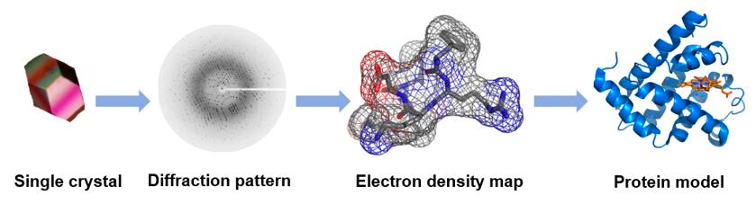
\includegraphics[width = 0.9\textwidth]{figs/paste-F430F5B1.png}
\caption{Flujo de trabajo esquemático de la cristalografía de rayos X. }
\label{fig:cristallography}
\end{figure}

Cuando recogemos datos de difracción de rayos X de un cristal, medimos las intensidades de las ondas difractadas dispersadas en todas las direcciones. Estas medidas nos dan las amplitudes, pero no la información de fase necesaria para reconstruir una imagen (mapa de densidad) de la molécula, lo que se conoce como el \textbf{«problema de fase»}. Este problema se agrava cuando faltan datos o éstos son deficientes. En la cristalografía de proteínas, las fases se obtienen a menudo utilizando las coordenadas atómicas de una proteína similar (reemplazamiento molecular, MR) o identificando las posiciones de los átomos pesados. Los átomos pesados dispersan los rayos X con más intensidad que los ligeros, lo que nos ayuda a determinar sus posiciones dentro del cristal. Comparando los patrones de difracción del cristal original y de uno con átomos pesados añadidos, podemos deducir información de fase mediante la sustitución isomorfa. Los átomos pesados actúan como puntos de referencia para recuperar la información de fase perdida, crucial para reconstruir la estructura tridimensional de la molécula. El reemplazo molecular encuentra modelos que se ajustan a las intensidades experimentales a partir de estructuras conocidas, para lo que suele ser necesario cubrir al menos el 50\% de la estructura total con una d.s.r.m. C$\alpha$ baja. Alrededor del 70\% o más de las estructuras PDB se han resuelto mediante este método (MR), y el número aumenta a medida que se dispone de más estructuras homólogas. Los avances en la predicción de estructuras proteicas de novo han dado lugar a protocolos como MR-Rosetta, QUARK, AWSEM-Suite, I-TASSER-MR y Alphafold-guided MR, que generan estructuras señuelo de tipo nativo útiles para resolver el problema de fase.

La difracción de rayos X es una potente técnica que permite obtener estructuras de alta resolución a nivel atómico de proteínas tanto solubles como de membrana, ya sean apoenzimas o holoenzimas unidas a un sustrato, cofactor o fármaco. Sin embargo, la muestra de proteína debe ser cristalizable (es decir, homogénea), lo que requiere una cantidad sustancial de proteína muy pura. Otra limitación de las estructuras de rayos X es que sólo proporcionan una (o muy pocas) formas estáticas de la proteína, y la localización de los átomos de hidrógeno no puede determinarse mediante métodos de difracción convencionales. Debido a su único electrón, los átomos de hidrógeno son difíciles de detectar con precisión con rayos X, que se dispersan en la densidad de electrones. Aunque los átomos de hidrógeno pueden predecirse, esta limitación sigue complicando algunos análisis químicos. Algunas proteínas conservan toda su funcionalidad, lo que permite realizar experimentos de cristalización con ciertas enzimas, pero también hay numerosos ejemplos en los que la cristalización puede conducir a una representación sesgada de la proteína y dar lugar a artefactos estructurales.

\subsection{Resonancia magnética nuclear}
Todos los núcleos atómicos son partículas cargadas que giran rápidamente y producen frecuencias de resonancia únicas para cada átomo. Cuando se aplica un campo magnético, puede detectarse una señal electromagnética con una frecuencia característica del campo magnético en el núcleo. Este principio constituye la base de la resonancia magnética nuclear (RMN, Figura \ref{fig/rmn}).

\begin{figure}[h]
\centering
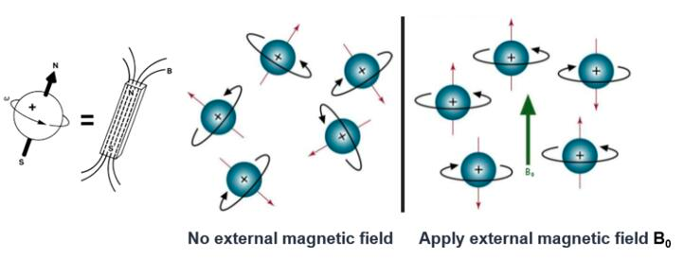
\includegraphics[width = 0.9\textwidth]{figs/paste-2013F0AC.png}
\caption{Bases de la resonancia magnética nuclear.}
\label{fig/rmn}
\end{figure}

Es importante señalar que el movimiento del núcleo no es aislado; interactúa tanto intra como intermolecularmente con los átomos circundantes. Por consiguiente, la espectroscopia de resonancia magnética nuclear puede proporcionar información estructural sobre moléculas específicas. Por ejemplo, en las proteínas, las estructuras secundarias como las $\alpha$-hélices, las $\beta$-hojas y los giros indican diversas disposiciones de los átomos de la cadena principal en el espacio tridimensional. Las distancias entre los núcleos atómicos en estas estructuras secundarias, sus interacciones y las propiedades dinámicas de los segmentos polipeptídicos revelan directamente la estructura tridimensional de las proteínas. Estas características nucleares contribuyen al comportamiento espectroscópico de la muestra, dando lugar a señales de RMN distintivas. La interpretación computacional de estas señales facilita la determinación de la estructura tridimensional de la proteína.

La principal ventaja del método de RMN es que permite medir directamente la estructura tridimensional de las macromoléculas en su estado natural en solución. La RMN proporciona información sobre la dinámica y las interacciones intermoleculares de estas moléculas. La resolución de la estructura tridimensional puede alcanzar el rango subnanométrico. Sin embargo, el espectro de RMN de biomoléculas grandes es complejo y difícil de interpretar, lo que limita su aplicación al análisis de biomoléculas grandes, normalmente por debajo de 20-30 kDa (Figura \ref{fig:molweight}). Además, esta técnica requiere cantidades relativamente grandes de muestras puras (varios miligramos) para lograr una relación señal-ruido razonable.

\begin{figure}[h]
\centering
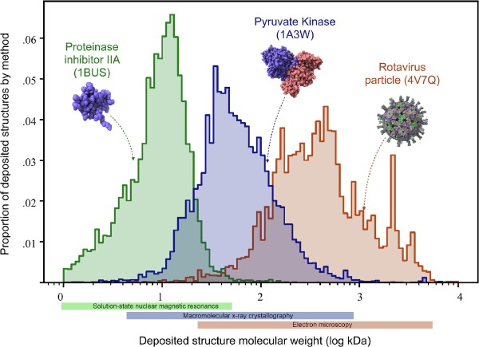
\includegraphics[width = 0.4\textwidth]{figs/paste-FA73AF1E.png}
\caption{Cobertura del peso molecular mediante la técnica estructural. }
\label{fig:molweight}
\end{figure}

\subsection{Criomicroscopía electrónica}
El principio fundamental de la crioEM es la dispersión de electrones, similar a otros métodos de microscopía electrónica. Las muestras se preparan mediante crioconservación antes del análisis. A continuación, se utiliza una fuente de electrones como fuente de luz para medir la muestra. Después de que el haz de electrones atraviese la muestra, un sistema de lentes convierte la señal dispersa en una imagen ampliada que se graba en el detector. Un paso posterior crucial es el procesamiento de la señal, que transforma miles de imágenes de las partículas en diversas orientaciones en una estructura tridimensional de la muestra.

\begin{figure}[h]
\centering
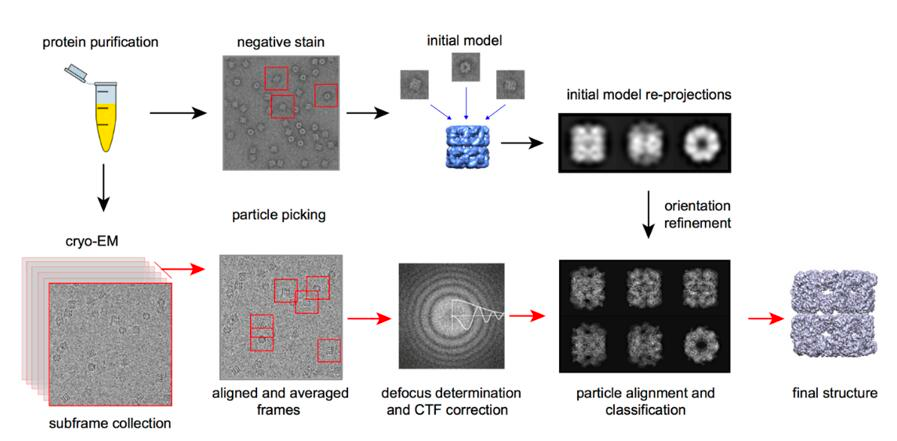
\includegraphics[width = 0.7\textwidth]{figs/paste-5E29F580.png}
\caption{El proceso de la técnica de análisis de partículas individuales Cryo-EM.}
\label{fig:cryoem}
\end{figure}

Tradicionalmente, el uso de métodos de microscopía electrónica para la biología estructural se limitaba a grandes complejos macromoleculares, como las cápsides víricas (Figura \ref{fig:molweight}). Recientemente, también se ha aplicado a partículas más pequeñas. El número de estructuras de proteínas determinadas mediante criomicroscopía electrónica ha aumentado considerablemente en los últimos 5-10 años (consultable en \href{https://www.rcsb.org/stats/all-released-structures}{PDB}). Este aumento se debe a varias mejoras técnicas de la técnica (Figura \ref{fig:cryo-rev}), como la preparación y conservación de muestras, el análisis y el procesamiento, que permiten obtener imágenes a nivel atómico. Estos avances fueron reconocidos con la concesión del Premio Nobel de Química 2017 a Jacques Dubochet, Joachim Frank y Richard Henderson .

\begin{figure}[h]
\centering
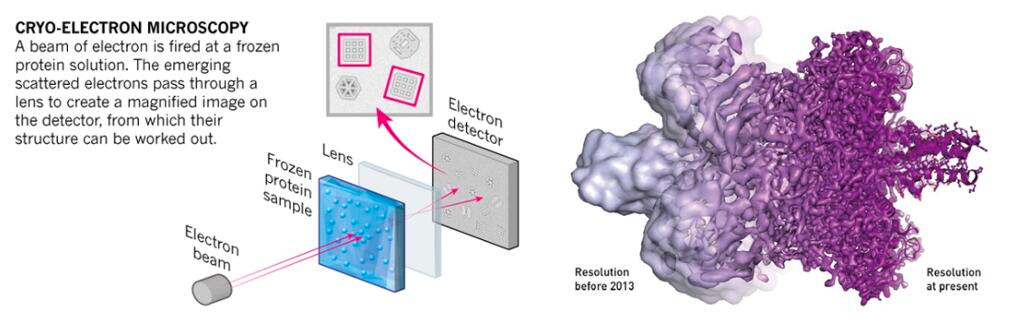
\includegraphics[width = 0.7\textwidth]{figs/paste-E5E5AE75.png}
\caption{La revolución de la criomicroscopía electrónica.}
\label{fig:cryo-rev}
\end{figure}

La crioEM se utiliza habitualmente hoy en día, sobre todo para grandes complejos moleculares o partículas víricas. Permite generar estructuras rápidamente, requiere una cantidad mínima de proteínas y puede producir datos fiables incluso con impurezas presentes. Sin embargo, los microscopios de nueva generación sólo suelen ser asequibles para las grandes instituciones, y las partículas pequeñas suelen tener un alto nivel de ruido. Además, procesar un gran número de imágenes puede suponer un reto cuando se pretende obtener estructuras de alta calidad.

\section{Garantía de calidad estructural}
Toda estructura, independientemente de su origen o método de determinación, es susceptible de error. Las estructuras determinadas experimentalmente son, en realidad, modelos que se han construido para alinearse con los datos experimentales. La calidad de los datos iniciales y la precisión de los procedimientos experimentales influyen significativamente en la fiabilidad de los resultados estructurales. Al igual que ocurre en otras disciplinas científicas, los experimentos independientes pueden dar lugar a modelos relacionados de la misma molécula, aunque suele haber variaciones; no obstante, ambos modelos pueden seguir considerándose representaciones exactas.

\subsection{Parámetros globales en estructuras basadas en experimentos}
Existen distintos parámetros que nos ayudan a comprender la calidad y fiabilidad de una estructura. En primer lugar, la \textbf{resolución} es un buen indicador del nivel de detalle de la estructura, ya que puede afectar en gran medida a la modelización de los datos experimentales.

\begin{figure}[h]
\centering
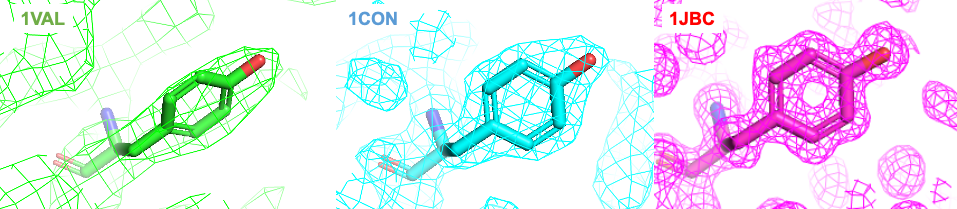
\includegraphics[width = 0.9\textwidth]{figs/paste-C3031EBE.png}
\caption{Efecto de la resolución en la calidad de la densidad electrónica. El residuo Tyr100 de la concanavalina A tal y como se encuentra en las estructuras PDB indicadas a 3 $\AA$, 2 $\AA$ y 1,2 $\AA$. }
\end{figure}

Otro parámetro importante es el \textbf{factor R}, que es la diferencia entre los factores de estructura calculados a partir del modelo y los obtenidos a partir de los datos experimentales. Es decir, el factor R es la desviación entre el patrón de difracción calculado del modelo y el patrón de difracción experimental original. Normalmente, las buenas estructuras con una resolución de 1-3 $\AA$, tienen un factor R de 0,2 (es decir, 20\% de desviación). Sin embargo, debe tenerse en cuenta que este factor suele reducirse tras el refinamiento iterativo, lo que resta importancia a su uso como indicador de fiabilidad. Un factor más fiable es el \textbf{factor$ R_{free}$}. Éste es menos susceptible de manipulación durante el refinamiento, ya que se basa sólo en una pequeña parte de los datos experimentales (5-10\%) que no se utiliza durante la fase de refinamiento.

Una forma más intuitiva, aunque sólo cualitativa, de entender la precisión de las coordenadas de un átomo determinado es el factor B. El valor de temperatura o factor B se correlaciona con los errores de posición, aunque su definición matemática es más compleja. Los valores normales de un factor B se sitúan entre 14 y 30, mientras que los valores superiores a 30 suelen indicar que el átomo se encuentra en una región flexible o desordenada, y los átomos con un factor B superior a 40 suelen descartarse por ser demasiado poco fiables.

La desviación cuadrática media (RMSD) es un estimador tradicional de la calidad de las estructuras resueltas por RMN. Las regiones con valores altos de RMSD (por encima de 6) son las que están menos definidas por los datos. Sin embargo, hay que tener en cuenta que este parámetro también puede ser engañoso, ya que depende en gran medida del procedimiento utilizado para generar y seleccionar los datos que se envían al PDB. Un experimentalista podría reducir la RMSD seleccionando las «mejores» pocas estructuras para su depósito a partir de un borrador mucho mayor. Además, la RMSD tiene muchas otras aplicaciones, como la comparación de diferentes estructuras o modelos de la misma secuencia o de secuencias relacionadas.

En los últimos años, con el aumento de la cantidad y la calidad de las estructuras EM, también se han propuesto nuevos parámetros. Uno de ellos, el \textbf{factor Q}, se introdujo recientemente para la \href{https://www.rcsb.org/news/feature/62de9e5235ec5bb4ddb19a43}{validación de estructuras 3DEM/PDB}. Brevemente, la puntuación del factor Q calcula la resolubilidad de los átomos midiendo la similitud de los valores del mapa alrededor de cada átomo en relación con una función tipo Gauss para un átomo bien resuelto. Una puntuación Q de 1 significa que la similitud es perfecta, mientras que un valor cercano a 0 indica una similitud baja. Si el átomo no está bien situado en el mapa, puede darse un valor Q negativo. Por lo tanto, los valores del factor Q en los informes oscilan entre -1 y +1.

\subsection{Parámetros estereoquímicos}
Dado que todos los modelos estructurales contienen cierto grado de error y que algunos de los parámetros globales de modelización pueden ser controvertidos, podemos analizar la geometría, la estereoquímica y otras propiedades estructurales del modelo para evaluar los modelos estructurales. Estos parámetros comparan una estructura dada con lo que ya se sabe sobre ese tipo de molécula a partir de nuestro conocimiento de las estructuras de alta resolución. Esto significa que las estructuras del espacio estructural actual definen lo que es «normal» en la estructura de una proteína. La ventaja de estos análisis y parámetros derivados es que no tienen en cuenta el proceso que conduce al modelo, sino sólo el producto final y su fiabilidad. La principal desventaja es que el espacio estructural actual se centra en proteínas con función conocida y de interés biomédico o biotecnológico.

Uno de los métodos más comunes y potentes para evaluar la estereoquímica de una proteína es el diagrama de Ramachandran, que se definió en 1963 y sigue utilizándose.

Otro análisis muy utilizado (disponible para todas las estructuras PDB) es el de los \textbf{ángulos de torsión de la cadena lateral}, medidos normalmente como \textbf{valores atípicos de la cadena lateral}. Las cadenas laterales de los aminoácidos también tienen algunas conformaciones preferidas. Al igual que el diagrama de Ramachandran, el diagrama de los ángulos de torsión $\chi$1-$\chi$2 puede indicar problemas con un modelo de proteína si los valores de los ángulos están fuera de los valores de alta densidad.

Los malos contactos o choques indican un modelo deficiente. Es obvio que dos átomos no pueden estar en el mismo lugar (o muy cerca). Podemos definir esto como una situación en la que dos átomos no unidos tienen una distancia entre centros menor que la suma de sus radios de van der Walls.

\section{Visualización de estructuras de proteínas}
\subsection{Formatos de ficheros de estructuras proteicas}
Los datos estructurales experimentales de diferentes métodos se almacenan en diferentes formatos de archivo. Por ejemplo, los datos cristalográficos en bruto suelen almacenarse como archivos \texttt{*.ccp4}, pero los mapas de densidad de Cryo-EM o rayos X pueden almacenarse en archivos \texttt{*.mrc} o \texttt{*.mtz}. Otros formatos de archivo complejos, como el Extensible Markup Language \texttt{*.xml}, proporcionan un marco para estructurar información compleja y documentos como estructuras de proteínas.

Junto con la creación del Banco de Datos de Proteínas, se desarrolló un formato sencillo y estandarizado. El formato Brookhaven o PDB consiste en registros de líneas en un formato fijo que describen coordenadas atómicas, características químicas y bioquímicas, detalles experimentales de la determinación de la estructura y algunas características estructurales como asignaciones de estructuras secundarias, enlaces de hidrógeno o sitios activos. La versión actual se denomina PDBx/mmCIF) también incorpora el formato de archivo de información cristalográfica ampliado (mmCIF), que permite la representación de estructuras de gran tamaño, química compleja y métodos experimentales nuevos e híbridos. Así, los archivos \texttt{*.pdb} y \texttt{*.cif} pueden considerarse idénticos.

\begin{figure}[h]
\centering
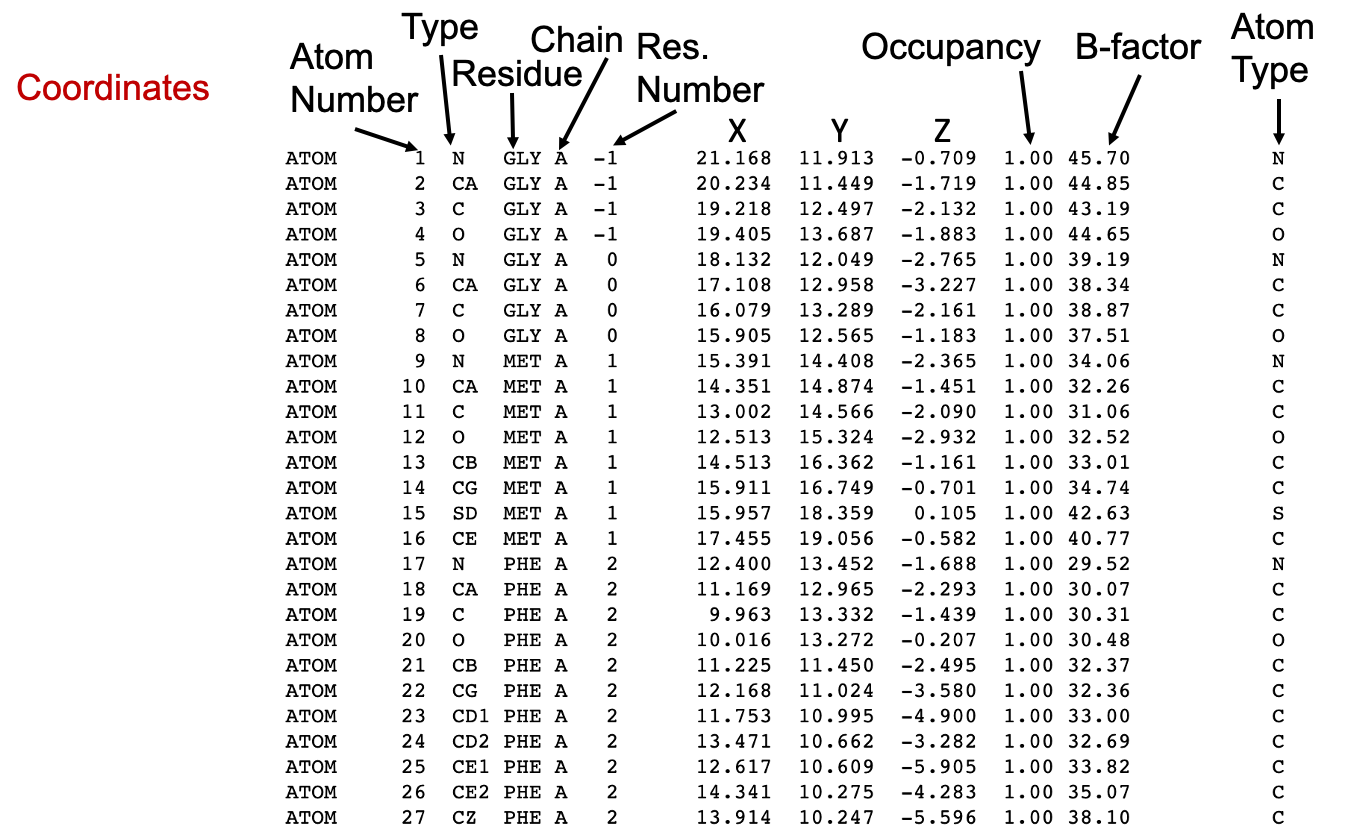
\includegraphics[width = 0.7\textwidth]{figs/coordinates-pdb.png}
\caption{Coordenadas en un fichero PDB.}
\end{figure}

\subsection{Ocupancia y factor B}
Excepto por la repetición del tipo de átomo en la columna de la derecha, las últimas columnas del archivo PDB son la \textbf{ocupancia} y el \textbf{factor de temperatura o el factor B}.

Los cristales macromoleculares están formados por muchas moléculas individuales empaquetadas en una disposición simétrica. En algunos cristales hay ligeras diferencias entre las moléculas individuales. Por ejemplo, una cadena lateral en la superficie puede oscilar entre varias conformaciones, o un sustrato puede unirse en dos orientaciones en un sitio activo, o un ion metálico puede detectarse unido sólo a algunas de las moléculas. Cuando los investigadores construyen el modelo atómico de estas porciones, pueden utilizar la ocupación para estimar la cantidad de cada conformación observada en el cristal. Por tanto, por definición, la suma de los \textbf{valores de ocupación} de cada átomo debe ser 1. Normalmente, vemos un único registro para un átomo, con un valor de ocupación de 1, lo que indica que el átomo se encuentra en todas las moléculas en el mismo lugar del cristal. Sin embargo, si un ion metálico se une sólo a la mitad de las moléculas del cristal, el investigador ve una imagen débil del ion en el mapa de densidad electrónica y puede asignar una ocupación de 0,5 para este átomo en el archivo de estructura PDB. Para cada átomo, se incluyen dos (o más) registros de átomos con ocupaciones tales como 0,5 y 0,5, o 0,4 y 0,6, u otras fracciones de ocupaciones que suman un total de 1.

Por otro lado, el \textbf{valor de temperatura o factor B} es una medida de nuestra confianza en la localización de átomos individuales, como se ha descrito anteriormente. Si encuentra un átomo con un factor de temperatura alto en la superficie de una proteína, tenga en cuenta que es probable que este átomo se mueva mucho y que las coordenadas dadas en el archivo PDB son sólo una posible instantánea de su ubicación. Así, un conjunto de datos de átomos con una ocupación < 1 puede tener un factor B bajo si esa posición es segura. 
Esta columna también es utilizada por los modelos derivados computacionalmente para indicar un valor de confianza que puede ser analizado para diversos fines, incluyendo la coloración de la estructura.

La metionina iniciadora siempre recibe el número de residuo de 1. Sin embargo, como a veces los cortes pueden no ser limpios, puede haber alguna cadena residual anterior a la metionina; estos reciben la numeración 0 y -1.

\subsection{Aplicaciones de visualización de macromoléculas biológicas}
\subsubsection{PyMOL}
PyMOL es un sistema de visualización molecular muy potente escrito originalmente por Warren DeLano. Fue lanzado en 2000 y pronto se hizo muy popular. Actualmente se comercializa bajo licencia de Schrödinger pero se puede solicitar una licencia libre para la enseñanza. Además, el código fuente abierto está disponible en GitHub que se puede instalar en Linux o MAC. 

PyMOL permite trabajar con diferentes representaciones de estructuras, pero también con datos experimentales brutos en diferentes formatos.

PyMOL está escrito en Python y puede ser usado con menús interactivos y también con línea de comandos. Hay muchos recursos que ayudan con PyMOL, como un Wiki de referencia de documentación o un PyMOLWiki soportado por la comunidad. Además, permite la implementación de nuevas funcionalidades como plugins, como PyMod o DockingPie, entre otros. PyMod está diseñado para actuar como interfaz simple e intuitiva entre PyMOL y varias herramientas bioinformáticas (i.e., PSI-BLAST, Clustal Omega, HMMER, MUSCLE, CAMPO, PSIPRED, y MODELLER). Partiendo de la secuencia de aminoácidos de la proteína diana, PyMod está diseñado para llevar a cabo los principales pasos del proceso de modelado homológico (es decir, la búsqueda de plantillas, la alineación de la secuencia diana-plantilla y la construcción del modelo) con el fin de construir un modelo atómico 3D de una proteína diana (o complejo proteico). La integración con PyMOL facilita un análisis detallado del proceso de modelado.

\subsubsection{UCSF ChimeraX}
ChimeraX es un software totalmente de código abierto, desarrollado por la UCSF como versión renovada del antiguo software Chimera, con versiones para Linux, MacOS y Windows. Pretende ser una herramienta integral de biología estructural, pero es más conocido por sus capacidades para mapas EM. Como cualquier otro software de código abierto, en los últimos años ha adquirido nuevas e interesantes capacidades, como la Realidad Virtual o el modelado Alphafold2.

\subsubsection{Estructuras moleculares en su sitio web: Mol* y otros}
LiteMol Viewer es una potente aplicación web HTML5 para la visualización 3D de moléculas y otros datos relacionados. Se utiliza en un navegador web, lo que elimina la necesidad de software externo y también permite la integración con sitios de terceros como un plugin incrustado. 

La misma filosofía se aplica a otros visores de código abierto que se desarrollaron más tarde y que ahora se utilizan más ampliamente, como NGL Viewer y Mol*, utilizados en los sitios RCSB-PDB y PDBe para la visualización 3D de estructuras. Con Mol* puede guardar la sesión de trabajo en formatos \texttt{molj} (sin las estructuras reales) o \texttt{molx} (con estructuras incrustadas).

Por último, para los científicos computacionales, también hay muchas bibliotecas que permiten la representación de moléculas en 3D, como la biblioteca 3Dmol Javascript y su envoltorio Python Py3Dmol, que se puede utilizar en Colab, Jupyter, Quarto o cualquier otro cuaderno Python.

Otra aplicación que se utilizaba, pero que ahora están descatalogada es SwissPDBViewer (también conocida como DeepView), desarrollada para trabajar con la aplicación de modelado homológico SWISS-MODEL. Es una aplicación que proporciona una interfaz fácil de usar que permite analizar varias proteínas al mismo tiempo. Actualmente ha caído en desuso ya que la última versión (4.1) es sólo una aplicación de 32 bits.


%12/02 - Modesto
\chapter{Modelado por homología}
\section{Modelización de estructuras proteicas: Cuidado con las diferencias}
El número de secuencias de proteínas en las bases de datos ha crecido exponencialmente en las últimas décadas, sobre todo tras la revolución de los métodos de secuenciación de alto rendimiento.

Sin embargo, la determinación experimental de estructuras tridimensionales de proteínas suele ser difícil, requiere mucho tiempo y está sujeta a limitaciones, como los errores experimentales, la interpretación de los datos y la modelización de nuevos datos sobre estructuras ya publicadas. Así, a pesar de los considerables esfuerzos iniciados a principios del siglo XXI para aplicar métodos de biología estructural de alto rendimiento, la disponibilidad de estructuras de proteínas es más de 1.000 veces inferior al número de secuencias. Por ejemplo, en febrero de 2025, hay ,más de 250 M de secuencias en Uniprot o más de 700 M de proteínas en MGnify, mientras que sólo alrededor de 220k estructuras en RCSB Protein Databank. Esta diferencia se denomina brecha secuencia-estructura de proteínas y se amplía constantemente, especialmente si consideramos las secuencias de las bases de datos de metagenómica no disponibles en Uniprot.

Así pues, para compensar la falta de datos experimentales es necesario predecir con precisión y fiabilidad la estructura tridimensional de una proteína determinada.

\section{¿Son predecibles las estructuras de las proteínas?}
Las propiedades de los aminoácidos determinan los ángulos $\Phi$ y $\Psi$ que acaban conformando los niveles estructurales superiores. Sin embargo, el plegamiento de proteínas puede ser más complejo, ya que debe acoplarse a la síntesis de proteínas.

Cabe imaginar que la complejidad y diversidad de las estructuras proteicas en la naturaleza puede ser enorme. De hecho, John Kendrew y sus colaboradores parecían muy decepcionados por la determinación de la primera estructura globular tridimensional, la mioglobina en 1958:
\begin{quote}
Quizá las características más notables de la molécula sean su complejidad y su falta de simetría. La disposición parece carecer casi por completo del tipo de regularidades que uno anticipa instintivamente, y es más complicada de lo que ha anticipado cualquier teoría de la estructura de las proteínas.
\end{quote}

No mucho más tarde, en 1968, Cyrus Levinthal (1922-1990) publicó la llamada paradoja de Levinthal, afirmando que las proteínas se pliegan en nano/milisegundos, pero incluso para los péptidos pequeños llevará un tiempo enorme probar el astronómico número de conformaciones posibles. Digamos que una proteína pequeña de 100 aminoácidos tiene 99 enlaces peptídicos y 198 ángulos $\Phi$ y $\Psi$ diferentes. Suponiendo sólo 3 conformaciones alternativas para cada enlace, se obtendrán $3^{198} (= 2,95 \times 10^{95})$ conformaciones posibles. Si diseñamos un algoritmo altamente eficiente que pruebe 1 conformación por nanosegundo:
$$2.95 \times 10^{85} \text{segundos} = 9 \times 10^{67} \text{mil millones de años}$$
Teniendo en cuenta que la edad del universo es de 13.800 millones de años, predecir las estructuras de las proteínas no parece tarea fácil.

En este contexto, un experimento muy sencillo realizado hace 50 años arrojó algo de luz sobre el mecanismo de plegamiento de las proteínas. Cristian Anfisen fue capaz de desnaturalizar (desdoblar) completamente la Ribonucleasa A, mediante la adición de agentes reductores y urea bajo tratamiento térmico, y posteriormente cambiar a condiciones normales que permiten a la proteína volver a plegarse de forma totalmente funcional. Este experimento indica que la secuencia de aminoácidos dicta la estructura final. A pesar de algunas excepciones relevantes, esto se ha confirmado en gran medida.
\begin{figure}[h]
\centering
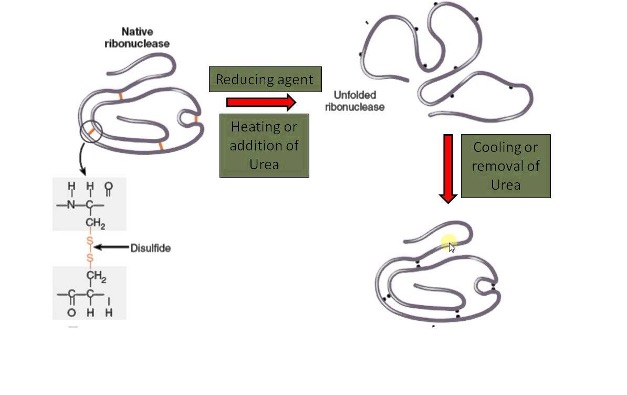
\includegraphics[width = 0.8\textwidth]{figs/anfinsen.jpg}
\caption{El dogma de Anfinsen: La secuencia de aminoácidos dictaba la estructura final. }
\end{figure}

Cabe imaginar que las estructuras nativas in vivo de las proteínas se parecen a la conformación más estable, es decir, al mínimo global de energía libre. Ésa es la base del modelo de embudo del plegamiento de proteínas, que supone que el número de conformaciones posibles se reduce cuando se alcanza un mínimo local de energía, lo que constituye un camino para el proceso de plegamiento.
\begin{figure}[h]
\centering
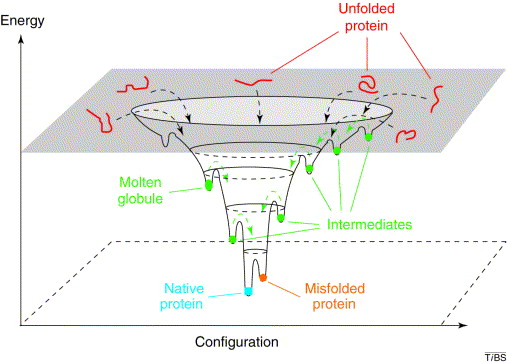
\includegraphics[width = 0.8\textwidth]{figs/funnel_1.jpeg}
\caption{Diagrama esquemático del paisaje energético de plegamiento de una proteína según el modelo del embudo. Las moléculas desnaturalizadas situadas en la parte superior del embudo pueden plegarse al estado nativo por una miríada de rutas diferentes, algunas de las cuales implican intermedios transitorios (mínimos energéticos locales), mientras que otras implican trampas cinéticas significativas (estados mal plegados).}
\end{figure}

\begin{table}[htbp]
\begin{mdframed}[backgroundcolor=black!10]
    \centering
    \textbf{Conclusión}: Se pueden predecir las estructuras de las proteínas porque sólo dependen de su secuencia. Pero para obtener predicciones precisas, o bien se necesita mucho tiempo y potentes ordenadores... o métodos realmente eficaces. 
    \end{mdframed}
\end{table}

El \textbf{modelado por homología} es uno de los trucos más convenientes para sortear esta limitación. Básicamente, la estrategia consiste en añadir más capas de información adicional a las propiedades de los aminoácidos, a saber, la conservación evolutiva de secuencias y estructuras.

Muy a menudo, antes de crear los modelos ya se dispone de cierta información sobre la proteína. Por ejemplo, si se trata de una enzima, es posible que se hayan descubierto los residuos catalíticos o la región de interacción con el sustrato. También es aconsejable buscar en la literatura, en particular para ver si hay un artículo complementario de la(s) estructura(s) PDB correspondiente(s) que pueda estar disponible o que pueda encontrar y utilizar como plantilla(s) para el modelado.

\section{Modelización comparativa: La conservación es la clave}
\begin{figure}[h]
\centering
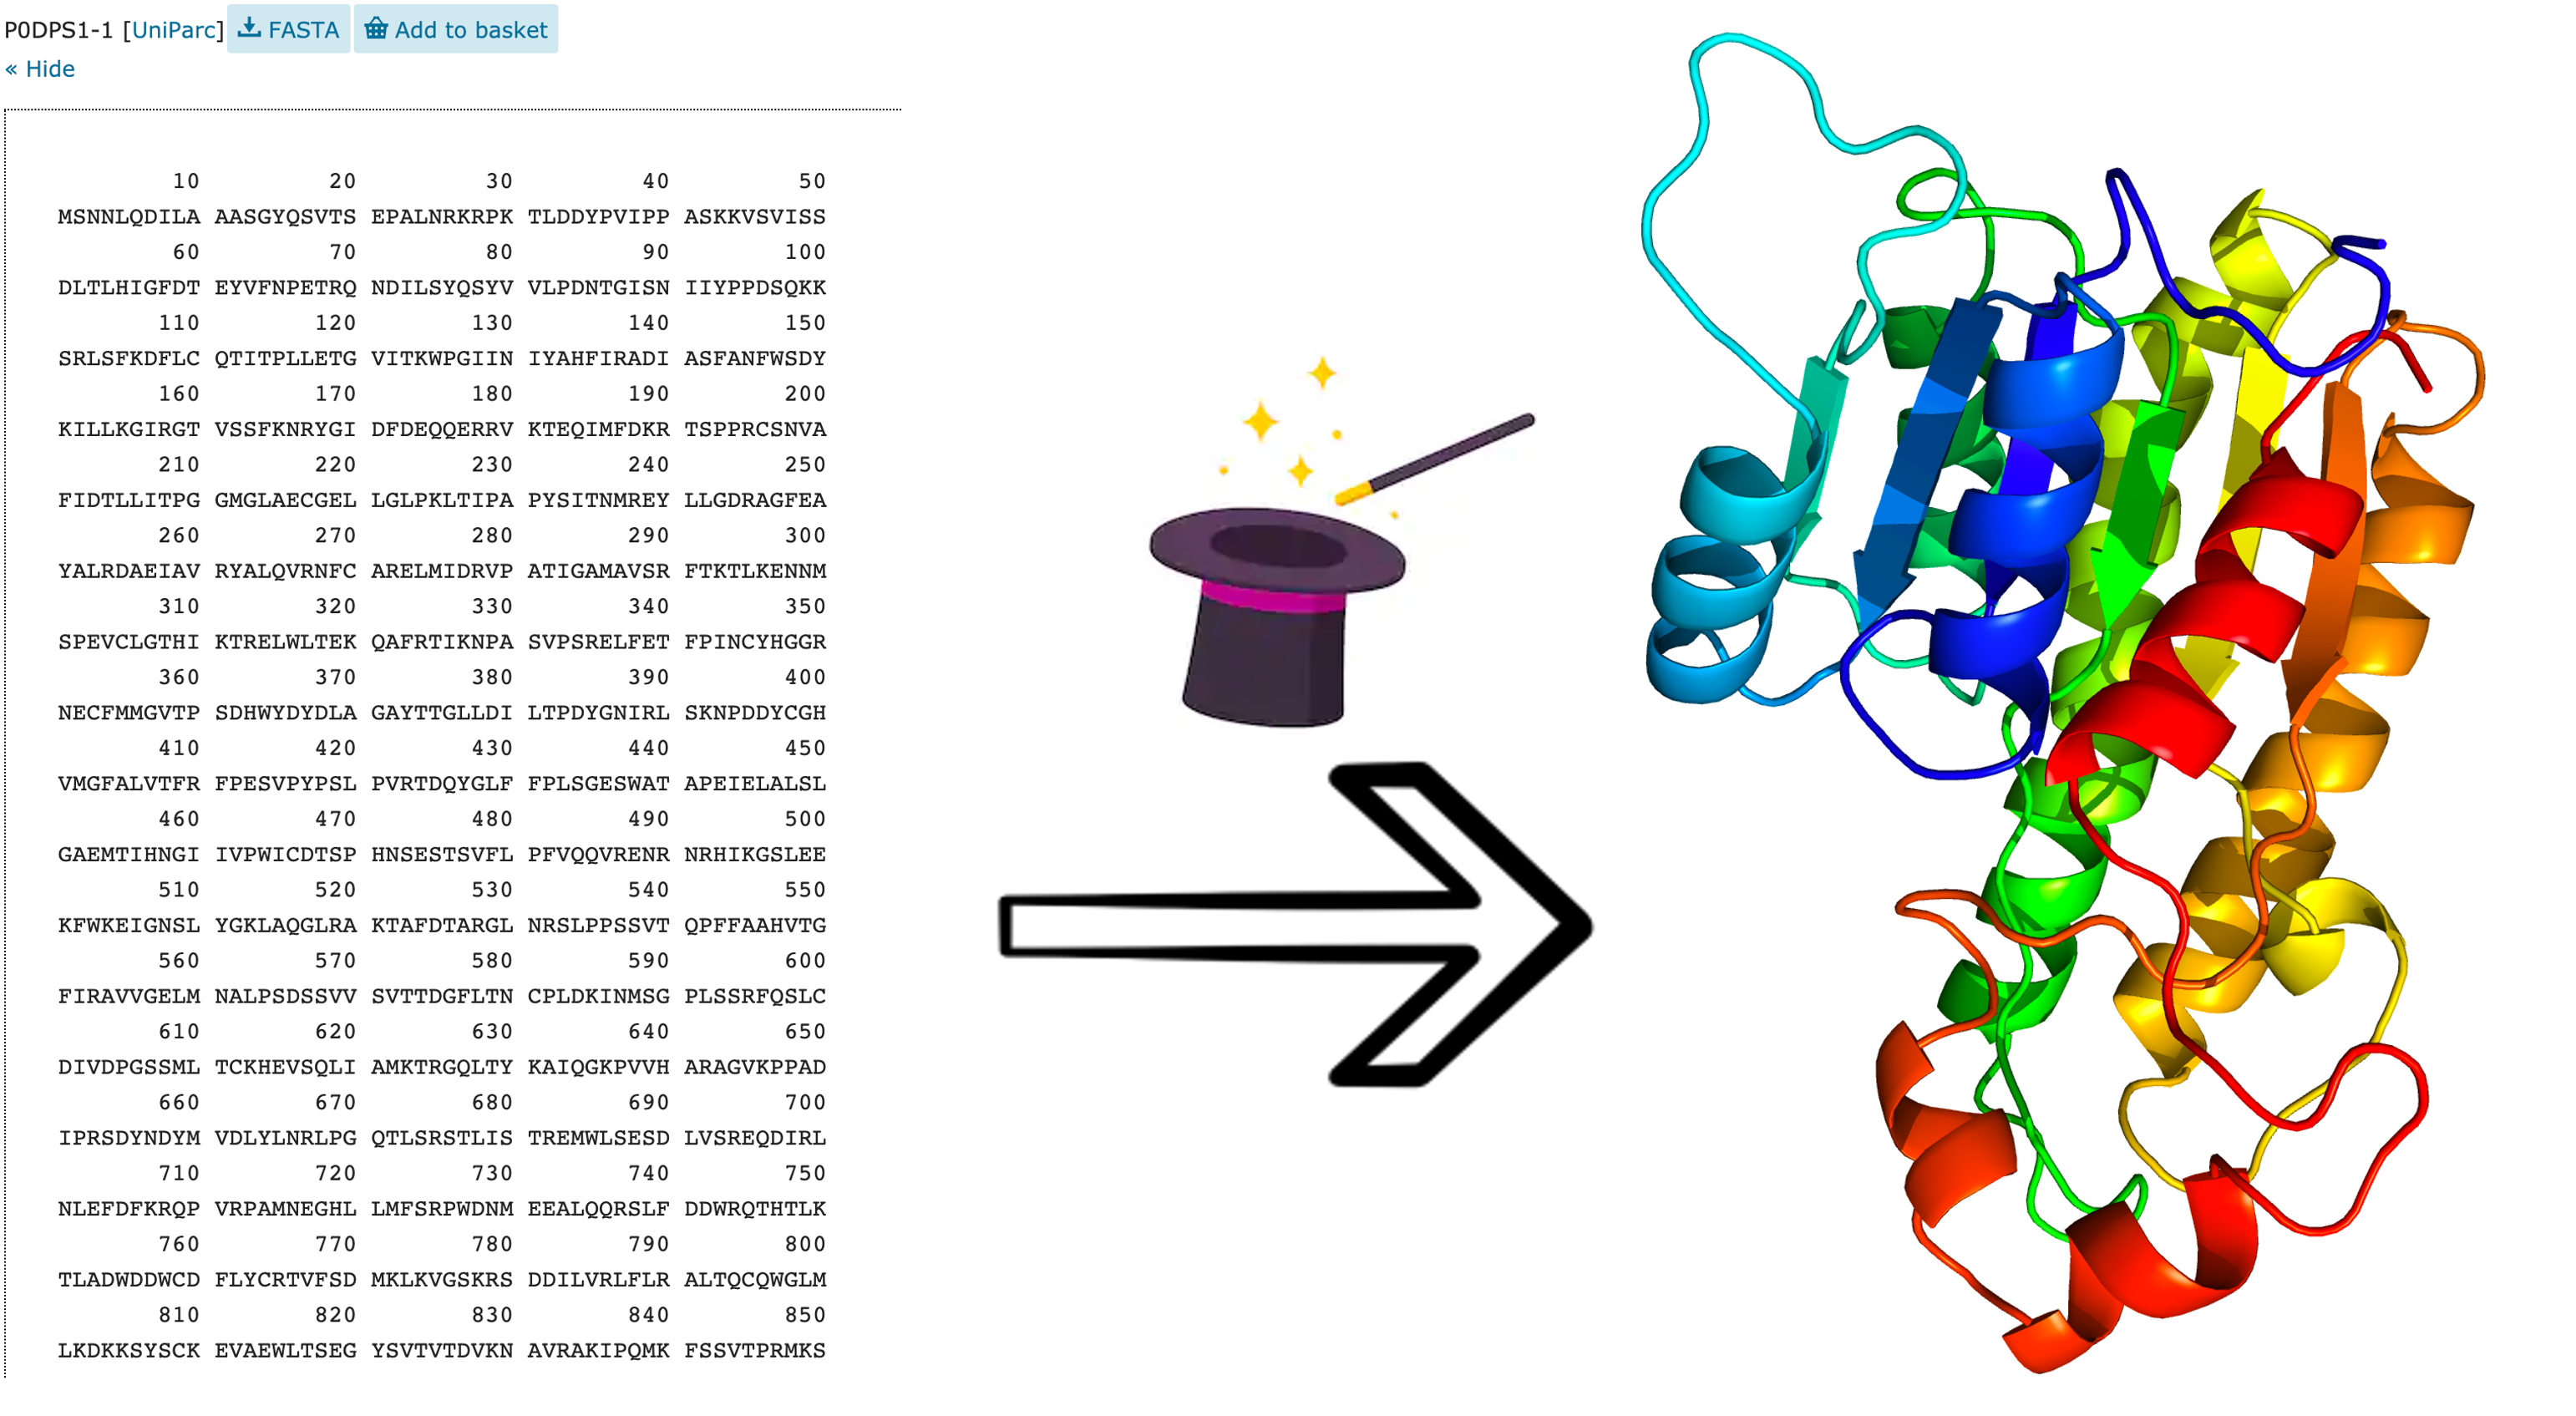
\includegraphics[width = 0.7\textwidth]{figs/modeling.png}
\caption{En pocas palabras, el modelado de proteínas consiste en pasar de la secuencia a la estructura. Pero, ¿cómo lo hacemos?}
\end{figure}

Tradicional y conceptualmente, la predicción de la estructura de las proteínas puede abordarse desde dos perspectivas diferentes: el modelado comparativo y la predicción \textit{ab initio}. En el enfoque del modelado comparativo, sólo se puede predecir la estructura tridimensional de secuencias de proteínas si se encuentran sus homólogas en la base de datos de proteínas con estructuras conocidas. Por supuesto, la identificación de tales homólogos es clave en este caso. Hasta hace poco, la mayor parte del desarrollo en el modelado de proteínas ha estado impulsado por el desarrollo de métodos para identificar similitudes de secuencias distantes que reflejarían pliegues proteicos similares. Por otra parte, el modelado \textit{ab initio} se basa únicamente en las propiedades fisicoquímicas de la molécula.

\begin{table}[htbp]
\begin{mdframed}[backgroundcolor=black!10]
    \centering
    Los términos «modelización homológica» y «modelización comparativa» suelen utilizarse indistintamente. Sin embargo, el modelado comparativo puede considerarse un enfoque más amplio que aprovecha las estructuras conocidas y abarca tanto el modelado homológico como el reconocimiento de pliegues o el enhebrado.
    \end{mdframed}
\end{table}

\begin{figure}[h]
\centering
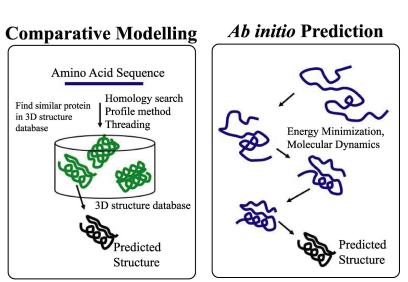
\includegraphics[width = 0.5\textwidth]{figs/predway.jpeg}
\caption{Dos enfoques diferentes para la predicción de estructuras.}
\end{figure}

El modelado homológico genera modelos estructurales basados en la estructura de (normalmente) una estructura homóloga relacionada. Así pues, la precisión del modelado homológico está limitada por la disponibilidad de estructuras similares. Las predicciones \textit{ab initio} están limitadas por los modelos matemáticos y los recursos informáticos, y a menudo sólo son útiles para péptidos pequeños.

Para mantener la estructura y la función, determinados aminoácidos de la secuencia proteica están sometidos a una mayor presión de selección. O bien evolucionan más despacio de lo esperado o dentro de ciertas restricciones, como la similitud química (es decir, sustituciones conservadoras). Por lo tanto, los enfoques de modelado homológico asumen que una secuencia proteica similar implica una estructura 3D y una función similares. De hecho, las proteínas en la naturaleza no parecen contener toda la diversidad posible. Así, aunque el número de secuencias y estructuras publicadas aumenta constantemente, el número de pliegues únicos se mantuvo casi constante desde 2008 hasta hace muy poco.

Esto significa que el espacio de secuencias de proteínas es mucho mayor que el espacio de estructuras. Algunas bases de datos, como Scop2 o CATH (Figura \ref{fig:cath}) han aprovechado esta circunstancia empleando clasificaciones jerárquicas de estructuras en un número limitado de categorías distintas. Entre 2006 y 2024, el número de dominios diferentes en CATH aumentó de 86.000 a 600.000, mientras que el número de arquitecturas se mantuvo relativamente estable en 40 y 43, respectivamente. Incluso después de analizar numerosas estructuras nuevas de la base de datos AlphaFold, sólo se identificaron 25 superfamilias nuevas (y ninguna arquitectura nueva) (Figura \ref{fig:cath2}).

\begin{figure}[h]
\centering
\includegraphics[width = 0.5\textwidth]{figs/cath.png}
\caption{Ejemplificaciones de las principales categorías de CATH en 2006.}
\label{fig:cath}
\end{figure}

\begin{figure}[h]
\centering
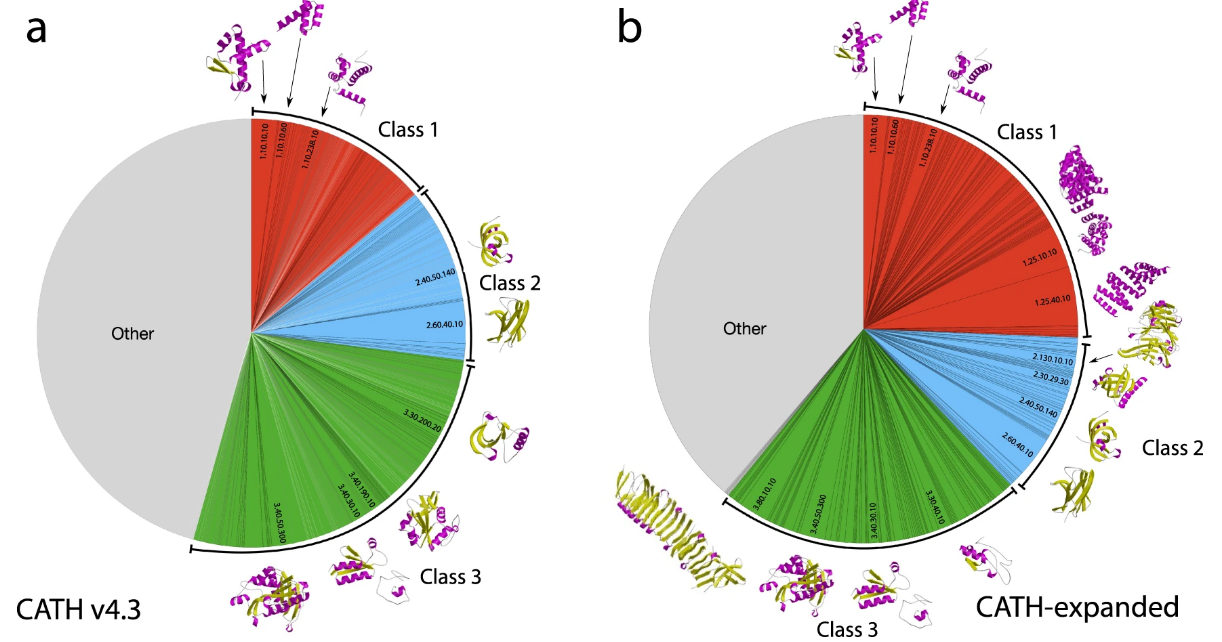
\includegraphics[width = 0.8\textwidth]{figs/cath2.png}
\caption{En 2022, la base de datos Alphafold amplió las principales categorías de CATH con 25 nuevas superfamilias.}
\label{fig:cath2}
\end{figure}

En resumen, las estructuras de las proteínas suelen estar más conservadas que sus secuencias, lo que permite construir modelos comparando proteínas con secuencias diferentes. Las secuencias biológicas evolucionan por mutación y selección, con una presión de selección variable para cada posición de residuo en una proteína en función de su importancia estructural y funcional. Los métodos de comparación de proteínas, como los alineamientos de secuencias, pretenden transmitir la historia evolutiva de las proteínas.

\section{Modelización homológica en cuatro pasos}
\begin{figure}[h]
\centering
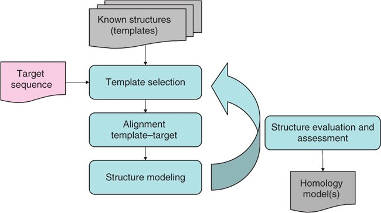
\includegraphics[width = 0.6\textwidth]{figs/homology_simple_workflow.png}
\caption{Flujo de trabajo del modelado de proteínas basado en una plantilla.}
\end{figure}

Un protocolo tradicional de modelización homológica construirá un modelo parcial o completo a partir de una secuencia de proeína basada en una única plantilla homóloga. En general, se requiere una identidad de secuencia mayor del 30\% entre la plantilla y la diana para obtener resultados fiables. Estos métodos requieren tres pasos (1) identificación de la plantilla más adecuada, (2) alineación de la secuencia de consulta y la plantilla, y (3) construcción del modelo. Estos pasos pueden abordarse con diferentes alternativas metodológicas y pueden arrojar diferentes resultados que deben evaluarse (paso 4) para encontrar la mejor solución para cada paso. 

En este curso, nos centraremos en el modelado de extremo a extremo utilizando SWISS-MODEL, un servidor de modelado totalmente automatizado que permite construir modelos sin necesidad de tener una sólida formación en bioinformática o conocimientos de programación. Las primeras versiones de SWISS-MODEL solo permitían el modelado de secuencias con homólogos en bases de datos, pero como se analiza a continuación, la implementación de avances en el reconocimiento de plantillas y la construcción de modelos ha aumentado la capacidad y la precisión del modelado, especialmente en los últimos 15 años.

SWISS-MODEL admite varias entradas. Normalmente, se introduce una consulta de secuencia única para la búsqueda de plantillas, pero también se puede omitir este paso e introducir directamente la plantilla deseada o incluso una plantilla y un alineamiento personalizado. Comenzaremos con la primera alternativa.

\subsection{Pasos 1 y 2: Búsqueda y alineación de plantillas}
\subsubsection{¿Dónde podemos buscar?}
La búsqueda de plantillas consiste en encontrar una proteína con estructura(s) conocida(s) con una secuencia relacionada con nuestra proteína. Como ya hemos mencionado, el Banco de Datos de Proteínas (PDB) del RCSB es la mayor base de datos de estructuras de proteínas. Así, podemos buscar plantillas comparando la secuencia de nuestra proteína con la secuencia de todas las proteínas del PDB. Sin embargo, el PDB se creó como repositorio para contener todas las estructuras macromoleculares, no para buscar plantillas para el modelado. Al igual que otros software de extremo a extremo, SWISS-MODEL tiene su propia base de datos curada, la SMLT (SWISS-MODEL template library). Se basa en alineaciones de perfiles del PDB, se actualiza semanalmente y también está anotada e indexada para facilitar la búsqueda. A día de 5 de febrero de 2025, SMLT contiene 158.703 secuencias de proteínas únicas que pueden mapearse en 386.135 unidades biológicas. Desde 2023, SWISS-MODEL también busca en la base de datos AlphaFold DB.

\subsubsection{¿Cómo podemos buscar de forma precisa y rápida?}
\begin{figure}[h]
\centering
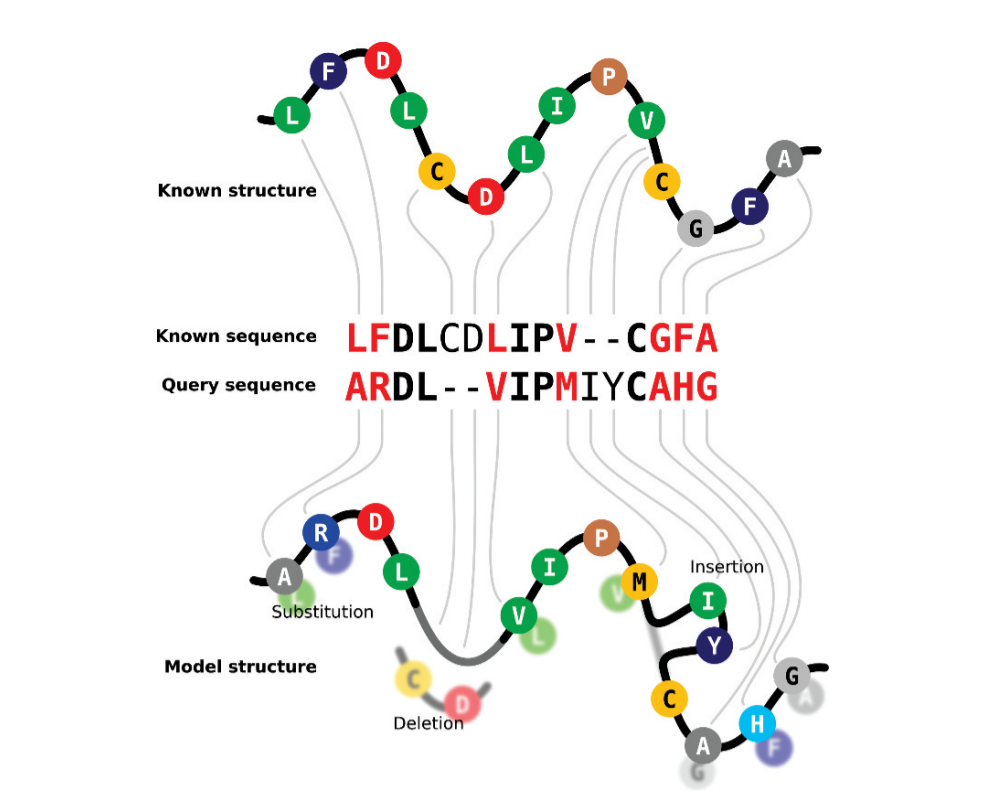
\includegraphics[width = 0.6\textwidth]{figs/template_query.png}
\caption{La alineación consulta-plantilla es la base del modelado homológico.}
\end{figure}

Para encontrar plantillas, hay que comparar secuencias, por lo que es esencial disponer de un método de alineación preciso y potente. Comparar la secuencia de una proteína con toda una base de datos lleva mucho tiempo porque se está comparando con proteínas completamente no relacionadas, lo que supone una pérdida de recursos. Dos mejoras fundamentales han aumentado la capacidad de búsqueda de plantillas: (1) la introducción de la estructura secundaria (SS) comparando las predicciones de SS de la proteína de consulta y las estructuras secundarias de la base de datos de proteínas, y (2) el uso de perfiles para facilitar la comparación. Los perfiles son un método matemático de resumir un alineamiento de secuencias múltiples que cuantifica la probabilidad de cada aminoácido en cada posición. Un tipo particular de perfil son los modelos de Markov ocultos (HMM), muy útiles para buscar secuencias similares en las bases de datos. También se modelan las probabilidades de transición (es decir, la probabilidad de que un aminoácido concreto siga a otro aminoácido concreto). 
Además, los HMM incluyen inserciones y deleciones de aminoácidos. Estas características permiten a los HMM modelar alineaciones enteras con gran detalle, incluidas regiones muy divergentes, y facilitan la identificación de posiciones muy conservadas que definen no sólo la función de las proteínas, sino también su plegamiento. Por ejemplo, residuos de glicina al final de cada cadena beta o un patrón de residuos polares que favorecen las hélices alfa. La comparación previa de la secuencia de consulta con una base de datos de secuencias nos permite incorporar información evolutiva sobre la secuencia. Así, pasamos de un requisito de más del 30\% de identidad para obtener buenos modelos antes de la implementación de perfiles, a buenos modelos incluso con $\sim$20\% de identidad o menos. Además, la generación de perfiles también facilita la agrupación de la base de datos de búsqueda, reduciendo el tiempo de búsqueda. La implementación de estas capacidades condujo a la implementación del llamado reconocimiento de pliegues en el modelado homológico.

\begin{figure}[h]
\centering
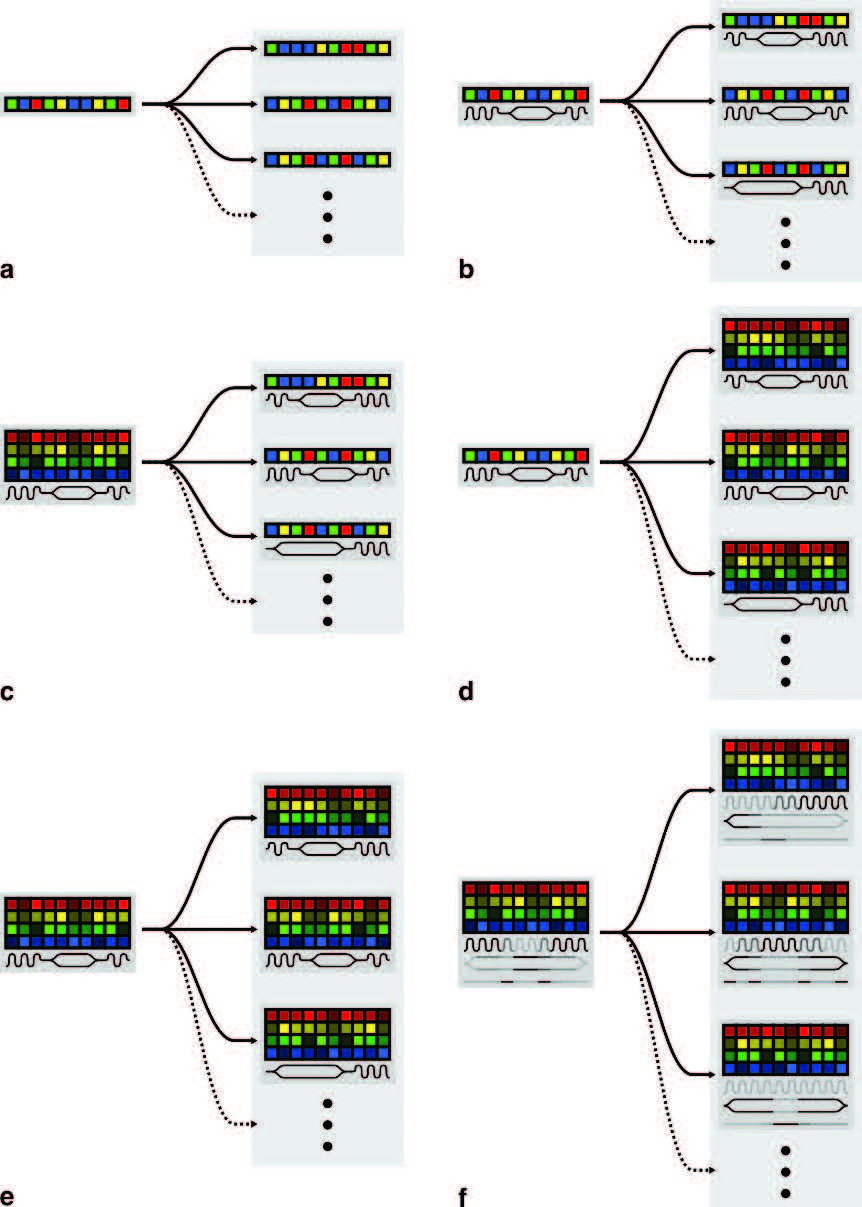
\includegraphics[width = 0.6\textwidth]{figs/profiles.jpg}
\caption{De la búsqueda secuencia contra secuencia a la comparación perfil-perfil.}
\end{figure}

La búsqueda de plantillas en SWISS-MODEL ha evolucionado a lo largo de los años hacia resultados más precisos. Actualmente, se realiza con \textbf{HHblits}, un método iterativo de perfil-perfil. También podemos buscar plantillas utilizando Blast u otros métodos de perfil-perfil, como Psi-BLAST, HHPred o JackHMMER. A continuación, las plantillas se clasifican entre 0 y 1 utilizando dos parámetros numéricos diferentes: \textbf{GMQE} (estimación global de la calidad del modelo) y \textbf{QSQE} (estimación de la calidad de la estructura cuaternaria). Brevemente, GMQE utiliza funciones de verosimilitud para evaluar varias propiedades de la alineación diana-plantilla (identidad de secuencia, similitud de secuencia, puntuación HHblits, concordancia entre la estructura secundaria predicha de la diana y la plantilla, concordancia entre la accesibilidad al disolvente predicha entre la diana y la plantilla; todo ello normalizado por la longitud de la alineación) para predecir la calidad esperada del modelo resultante. QSQE evalúa la probabilidad del estado oligomérico del modelo.

\subsection{Paso 3: Construcción del modelo}
Por defecto, SWISS-MODEL proporcionará 50 posibles plantillas clasificadas. La salida también contiene información sobre el método y la resolución de las plantillas, el porcentaje de identidad (y la cobertura de la alineación) con la secuencia de consulta, y el GMQE y QSQE.

La plantilla superior está marcada por defecto y es probable que dé el mejor modelo, pero también es interesante probar algunas plantillas alternativas dependiendo de la aplicación posterior del modelo. Por ejemplo, con un sustrato/cofactor diferente que pueda tener un papel clave en la función de la proteína o con una cobertura o porcentaje de identidad diferente.

Una vez seleccionada(s) la(s) plantilla(s), se construyen las coordenadas del modelo basándose en la alineación de la secuencia de consulta y de la plantilla utilizando el módulo ProMod3. SWISS-MODEL utiliza un ensamblaje de fragmentos, que es también la base de los métodos Fold-recognition o Threading. Otros programas, como Modeller, se basan en la satisfacción de restricciones espaciales generales. Modeller es una herramienta de línea de comandos que permite la personalización completa del modelado, lo que requiere más conocimientos sobre el proceso pero puede ser muy útil para algunos tipos de proteínas. No obstante, se ha implementado en algunos servidores en línea (ModWeb), cuadernos de Python y aplicaciones de fácil uso, como ChimeraX y Pymol (plugin Pymod). Modeller también se puede llamar desde la salida de HHPred (si se incluyó PDB como base de datos de búsqueda), lo que es muy conveniente para modelar homólogos remotos utilizando varias plantillas en pocos minutos.

El ensamblaje de fragmentos utilizará los átomos de la columna vertebral del núcleo de la plantilla para construir una estructura central del modelo, dejando las regiones no conservadas (principalmente bucles) para más adelante. El \textbf{modelado de bucles} incluye el uso de un subconjunto de homólogos de una base de datos de bucles específica, el muestreo de Monte Carlo como alternativa e incluso la construcción \textit{ab initio} de bucles que faltan.

\begin{figure}[h]
\centering
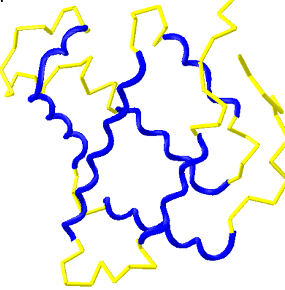
\includegraphics[width = 0.4\textwidth]{figs/loops.png}
\caption{Modelado de backbone y loop.}
\end{figure}

A continuación, se procede al posicionamiento de la \textbf{cadena lateral} de los aminoácidos no conservados. El objetivo es encontrar la conformación más probable de la cadena lateral, utilizando la información de la estructura plantilla, las bibliotecas de rotámeros (de un conjunto curado de estructuras de proteínas conocidas) y criterios energéticos y de empaquetamiento. Si hay que colocar muchas cadenas laterales en la estructura, se producirá el «problema del huevo y la gallina», ya que la colocación de un rotámero afectaría a los demás. Eso significa que la identificación de posibles enlaces de hidrógeno entre las cadenas laterales de los residuos y entre las cadenas laterales y la columna vertebral reduce los cálculos de optimización. Al fin y al cabo, cuantos más residuos se posicionen correctamente, mejor será el modelo.

\begin{figure}[h]
\centering
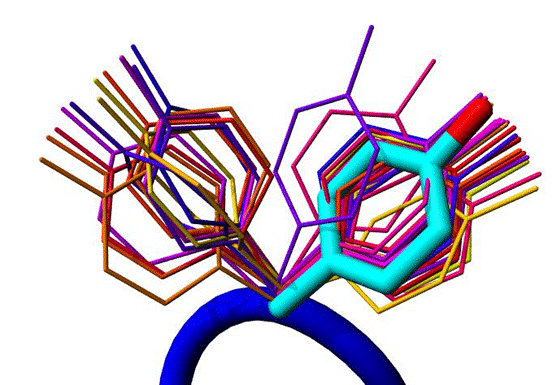
\includegraphics[width = 0.5\textwidth]{figs/Rotamers.png}
\caption{Modelado de cadena lateral.}
\end{figure}

Por último, se lleva a cabo una breve minimización de la energía para reducir los contactos y enlaces desfavorables adaptando las geometrías angulares y relajando los contactos cercanos. Este paso de minimización de energía o refinamiento puede ser útil para conseguir mejores modelos, pero sólo cuando el plegamiento ya es preciso.

\subsection{Paso 4: Evaluación de resultados}
El ordenador siempre te da un modelo, pero eso no significa que tenga un modelo que tenga sentido. ¿Cómo podemos saber si podemos fiarnos del modelo? Los modelos de salida están coloreados en una escala de colores de temperatura, del azul marino (buena calidad) al rojo (mala calidad). Eso puede ayudarnos a entender nuestro modelo a primera vista. Además, se trata de un sitio interactivo y se puede acercar y alejar el modelo. Hay muchas otras funciones disponibles para trabajar en tu modelo. Por ejemplo, puedes comparar varios modelos, puedes cambiar las opciones de visualización. También puedes descargar todos los archivos e informes en el botón «Datos del proyecto».

También existe la opción «Evaluación de la estructura». Esta opción proporciona un informe detallado de los problemas estructurales de su modelo. Se pueden ver gráficos de Ramachandran que resaltan en rojo los residuos de aminoácidos con ángulos phi/psi anormales en el modelo y una lista detallada de otros problemas.

El GMQE se actualiza con la puntuación QMEAN Z y QMEANDisCo (Studer et al. 2020). La puntuación QMEAN Z o la puntuación QMEAN normalizada indica cómo se compara el modelo con estructuras experimentales de tamaño similar. Una puntuación QMEAN Z en torno a 0 indica una buena concordancia, mientras que las puntuaciones por debajo de -4,0 se dan a modelos de baja calidad. Además del número, un gráfico muestra la puntuación QMEAN de nuestro modelo (estrella roja) dentro de todas las puntuaciones QMEAN de estructuras determinadas experimentalmente en comparación con su tamaño. En general, la puntuación Z equivale a la desviación estándar de la media.

\begin{figure}[h]
\centering
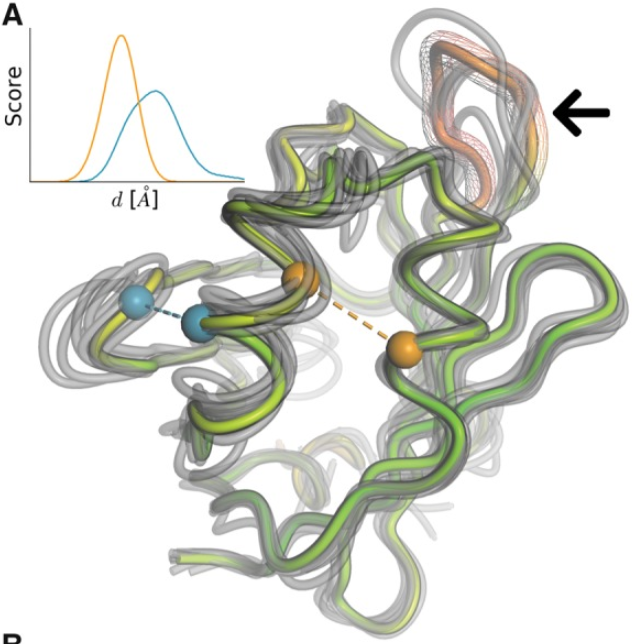
\includegraphics[width = 0.5\textwidth]{figs/paste-C2BED0C6.png}
\caption{Las puntuaciones QMEANDisCo por residuo se representan como un gradiente de color rojo a verde en un modelo de lbp-8 en \textit{Caenorhabditis elegans} (UniProtKB: O02324, PDB: 6C1Z). Las restricciones de distancia se han construido a partir de un conjunto de estructuras proteicas determinadas experimentalmente que son homólogas a lbp-8. El recuadro muestra dos ejemplos de restricciones entre residuos marcados con esferas de colores en el modelo. }
\end{figure}

El QMEANDisCO se implementó en SWISS-MODEL en 2020 y es un potente parámetro único que combina potenciales estadísticos y términos de acuerdo con una restricción de distancia (DisCo) para proporcionar una puntuación de consenso. DisCo evalúa la consistencia de las distancias CA-CA por pares de un modelo con restricciones extraídas de estructuras homólogas. Todas las puntuaciones se combinan utilizando una red neuronal entrenada para predecir puntuaciones por residuo. Podemos comprobar una puntuación global, pero también una puntuación local para cada residuo, que nos ayudan a comprender qué regiones del modelo tienen más probabilidades de plegarse con precisión (es decir, son más fiables).

\href{https://swissmodel.expasy.org/assess}{Swissmodel Assessment} también se puede utilizar como herramienta externa para analizar modelos obtenidos con otros métodos con el fin de hacerlos comparables, sólo necesita archivos .pdb de su modelo y, opcionalmente, la proteína modelo de referencia.

Existen otras herramientas independientes de evaluación de modelos que se utilizan habitualmente para evaluar modelos de proteínas, como VoroMQA o MoldFold. VoroMQA es un método muy rápido que combina la idea de potenciales estadísticos (es decir, una función de puntuación basada en el conocimiento) con el uso de áreas de contacto interatómico para proporcionar una puntuación en el rango de [0,1]. Cuando se aplica a la base de datos PDB, la mayoría de las estructuras de alta calidad basadas en experimentos tienen una puntuación VoroMQA >0,4. Por lo tanto, si la puntuación es superior a 0,4, es probable que el modelo sea bueno y los modelos con una puntuación <0,3 son probablemente malos. Los modelos con una puntuación de 0,3-0,4 son inciertos y no deben clasificarse con VoroMQA. Por otro lado, ModFold es una metaherramienta que le proporciona un informe muy detallado (y archivos parseables) con puntuaciones locales y globales, pero puede tardar horas/días en obtener el resultado, por lo que tendemos a utilizarla sólo con modelos seleccionados.

Otro parámetro clave que debe conocer si desea comparar estructuras de proteínas es el \textbf{RMSD del carbono alfa}. Cualquier alineamiento estructural de proteínas le dará este parámetro como estimación de la diferencia de las estructuras. Puede alinear estructuras con muchos servidores online, como RCSB, FATCAT2 o usando aplicaciones de visualización molecular, incluyendo Mol*, ChimeraX o PyMOL.

\subsection{Corolario: ¿Qué puedo hacer con mi modelo y qué no?}
\begin{figure}[h]
\centering
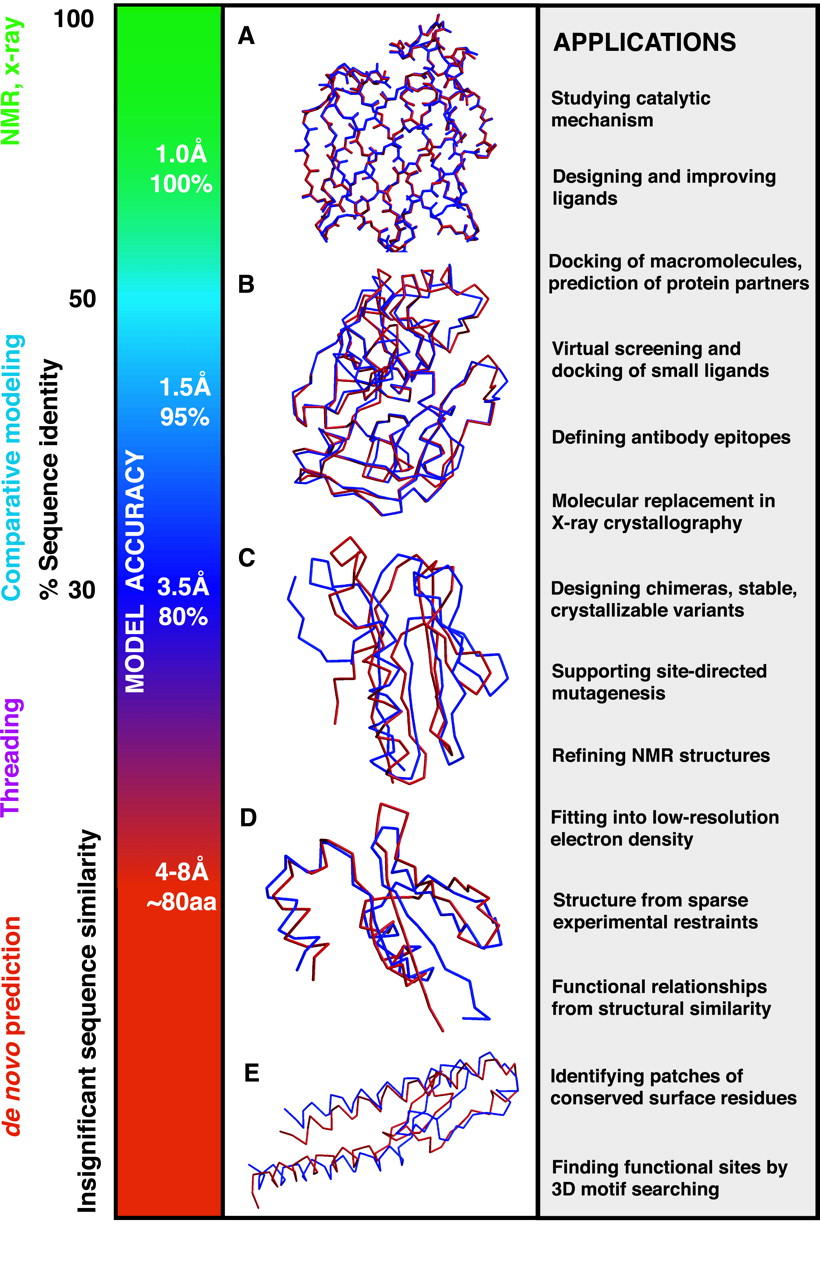
\includegraphics[width = 0.8\textwidth]{figs/sali.jpeg}
\caption{Precisión y aplicación de los modelos de estructura de proteínas (en 2001).}
\end{figure}

Un gran poder conlleva una gran responsabilidad. El uso de modelos conlleva una precaución y una necesidad de validación experimental. Sin embargo, conocer las limitaciones de nuestro modelo es necesario para un uso realista del mismo; y los límites vienen definidos por la calidad del modelo.

La precisión de un modelo comparativo está relacionada con el porcentaje de identidad de secuencia en el que se basa. Los modelos comparativos de alta precisión pueden tener un error cuadrático medio (RMS) de aproximadamente 1-2 $\AA$ para los átomos de la cadena principal, lo que es comparable a la precisión de una estructura de resonancia magnética nuclear (RMN) o una estructura de rayos X. Estos modelos pueden utilizarse para estudios funcionales y la predicción de socios de proteínas, incluidos fármacos u otras proteínas que trabajen en el mismo proceso. Además, para algunos estudios detallados, sería conveniente refinar su modelo mediante Dinámica Molecular y métodos afines hacia una estructura similar a la nativa. 

Por el contrario, los modelos comparativos de baja precisión se basan en una identidad de secuencia inferior al 20-30\%, lo que dificulta la capacidad de modelado y la precisión. Algunos de estos modelos pueden utilizarse con fines de ingeniería de proteínas o para predecir la función de secuencias huérfanas basándose en el pliegue de la proteína (utilizando Dali o Foldseek).

%14/02 - Modesto
\chapter{Características 1D}
Las características 1D son características de la proteína que pueden interpretarse directamente a partir de la secuencia primaria de la proteína y representarse como valores asignados a cada residuo de la secuencia. Por ejemplo, podemos asignar un estado de estructura secundaria (símbolo o probabilidad) a cada residuo. Muchos métodos de predicción de estructuras utilizan o incorporan métodos de terceros para predecir la estructura secundaria y otras características 1D, que proporcionan información crucial durante el proceso de modelado.

\section{Predicción de la estructura secundaria de proteínas}
\subsection{Estado múltiple de las estructuras secundarias}
Las estructuras secundarias se asignan a estructuras utilizando el \textbf{algoritmo DSSP (Define Secondary Structure of Proteins)}, creado originalmente en 1983 y actualizado varias veces, con la última versión disponible en GitHub desde 2021. El algoritmo DSSP clasifica cada residuo en función de su geometría y de los enlaces de hidrógeno previstos, comparándolos con los patrones de la base de datos DSSP. Es importante destacar que DSSP no predice estructuras secundarias; simplemente extrae esta información de las coordenadas 3D. DSSP no es una predicción.

La mayoría de los métodos de predicción de estructuras secundarias de proteínas (PSSP) utilizan un modelo de tres estados, que clasifica las estructuras secundarias en hélice (H), lámina (E) y espiral (C). La hélice y la lámina son las principales conformaciones propuestas por Linus Pauling en los inicios de la biología estructural, mientras que la bobina (C) se refiere a cualquier aminoácido que no encaje en las categorías de hélice o lámina. Este modelo de tres estados sigue siendo muy utilizado, pero tiene limitaciones, ya que simplifica en exceso la estructura de la columna vertebral y a menudo omite las desviaciones de las conformaciones estándar de hélice y lámina.

En la década de 1980, se propuso un modelo de estructura secundaria de ocho estados, incluyendo $\alpha$-hélice (H), 310-hélice (G), $\beta$-hoja paralela/antiparalela (E), $\beta$-puente aislado (B), pliegue (S), giro (T), $\pi$-hélice (I) y espiral (C). DSSP define estos ocho estados en estructuras obtenidas experimentalmente e incluye transformaciones para mapear estructuras de ocho estados a modelos de tres estados.

Más recientemente, en 2020, se introdujeron modelos PSSP de cuatro y cinco estados para simplificar las predicciones y aumentar la precisión. Estos nuevos modelos abordan el desequilibrio en el tamaño de las muestras para determinadas clases, como el puente $\beta$ aislado (B) y el pliegue (S), que tienen menos muestras y menores tasas de verdaderos positivos. En el modelo de cinco estados, B y S se categorizan como C, mientras que en el modelo de cuatro estados, B, S y G se categorizan como C. Además, el 75\% de las apariciones de $\pi$-hélices (I) se encuentran al principio o al final de una $\alpha$-hélice (H), por lo que se categorizan como H. Aún se está explorando todo el potencial de estas nuevas categorías.

\subsection{Evolución de los métodos de predicción}
La predicción de la estructura secundaria de proteínas (PSSP) a partir de secuencias proteicas se basa en la idea de que segmentos de residuos consecutivos tienen preferencias por determinados estados de estructura secundaria. Al igual que otros métodos bioinformáticos, incluido el modelado de proteínas, los métodos de predicción de estructuras secundarias han evolucionado en los últimos 50 años.

Los métodos de primera generación se basaban en enfoques estadísticos, en los que la predicción dependía de asignar un conjunto de valores de predicción a un residuo y aplicar después un algoritmo sencillo a esos números. Esto significaba aplicar una puntuación de probabilidad basada en la propensión de un solo aminoácido. En los años 90, nuevos métodos incluyeron la información de los residuos flanqueantes (3-50 aminoácidos cercanos) en los llamados métodos del vecino más próximo (N-N). Estos métodos aumentaron la precisión en muchos casos, pero seguían teniendo fuertes limitaciones, ya que sólo consideraban tres estados posibles (hélice, hebra o giro). Además, como se sabe por la práctica de la estructura secundaria, las predicciones de $\beta$-cadenas son más difíciles y no mejoraron mucho gracias a los métodos N-N. Además, las hélices y hebras predichas solían ser demasiado cortas.

A finales de los años 90, nuevos métodos elevaron la precisión a valores cercanos al 80\%. Estos métodos incluían dos innovaciones, una conceptual y otra metodológica. La innovación conceptual fue la inclusión de información evolutiva en las predicciones, mediante la consideración de la información de alineamientos o perfiles de secuencias múltiples. Si un residuo o un tipo de residuo se conserva evolutivamente, es probable que sea importante para definir tramos de estructura secundaria. La innovación metodológica fue el uso de redes neuronales, en las que se compararon múltiples capas de predicciones secuencia-estructura con redes entrenadas independientemente.

Desde la década de 2000, los métodos más utilizados son los metiservidores que comparan varios algoritmos, en su mayoría basados en redes neuronales, como JPred o SYMPRED, entre otros.

En los últimos años, las redes neuronales profundas entrenadas con grandes conjuntos de datos se han convertido en el método principal para la predicción de estructuras secundarias de proteínas (y casi cualquier otra predicción en biología estructural). En la era Alphafold, también se utilizan métodos adaptados del procesamiento de imágenes o del procesamiento del lenguaje natural (PLN) (por ejemplo, en NetSurfP-3.0), lo que permite que las predicciones de estructuras secundarias de proteínas se centren en objetivos específicos, como mejorar la calidad de la información evolutiva para el modelado de proteínas.

\section{Desorden estructural y accesibilidad de los disolventes}
El desorden de expresión denota tramos de proteína que no pueden asignarse a ningún SS. Suelen ser dinámicos/flexibles, por lo que presentan un elevado factor B o incluso faltan en las estructuras cristalinas. Estos fragmentos muestran una baja complejidad y suelen ser ricos en residuos polares, mientras que los residuos aromáticos rara vez se encuentran en regiones desordenadas. Estos motivos suelen encontrarse en los extremos de las proteínas o en los límites de los dominios (como enlazadores). Además, suelen estar relacionados con funcionalidades específicas, como en el caso de dianas proteolíticas o interacciones proteína-proteína (PPI). Más raramente, grandes dominios desordenados pueden conservarse en familias de proteínas y asociarse a funciones relevantes, como en el caso de algunos factores de transcripción, reguladores de transcripción, quinasas...

Existen muchos métodos y servidores para predecir regiones desordenadas. El servidor más conocido es DisProt, que utiliza una gran base de datos curada de proteínas intrínsecamente desordenadas y regiones de la literatura, que se ha mejorado recientemente a la versión 9 en 2022.

El colapso hidrofóbico suele considerarse un paso clave en el plegamiento de las proteínas. Los residuos hidrófobos tienden a quedar enterrados en el interior de la proteína, mientras que los aminoácidos polares e hidrófilos quedan expuestos al disolvente acuoso.

\begin{figure}[h]
\centering
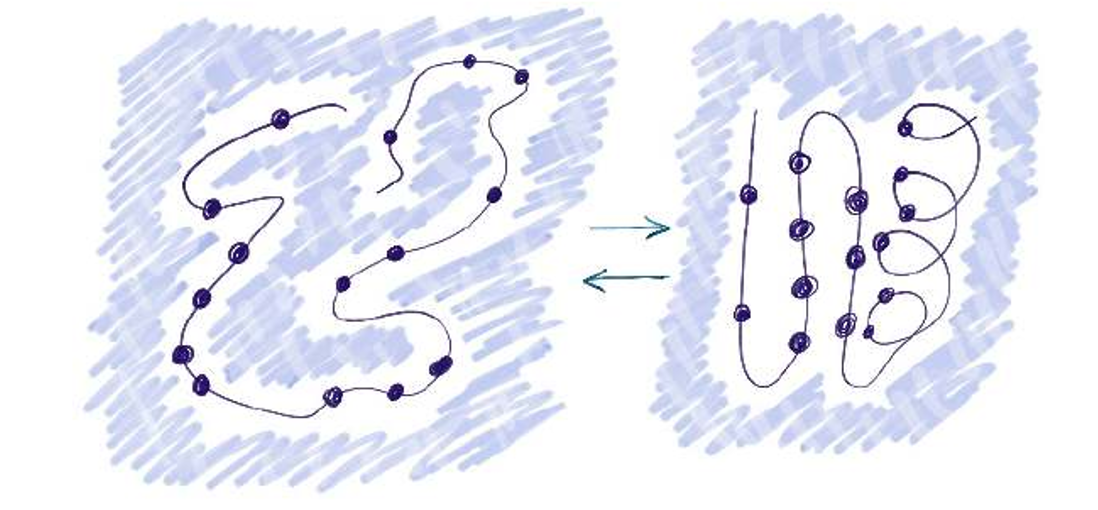
\includegraphics[width = 0.8\textwidth]{figs/collapse.png}
\caption{El colapso hidrofóbico como paso inicial en el plegamiento de proteínas.}
\end{figure}

La accesibilidad al disolvente se correlaciona con la hidrofobicidad de los residuos (los métodos de accesibilidad suelen ofrecer mejores resultados). Por lo tanto, la estimación de la probabilidad de que cada residuo esté expuesto al disolvente o enterrado dentro de la proteína es útil para obtener y analizar modelos de proteínas. Además, esta información es útil para predecir PPIs, así como la unión de ligandos o sitios funcionales. La mayoría de los métodos sólo clasifican cada residuo en dos grupos: Enterrados, para aquellos con probabilidad de accesibilidad relativa <16\% y Expuestos, para residuos de accesibilidad >16\%.

Los métodos recientes más comunes, como ProtSA o PROFacc, combinan información evolutiva con redes neuronales para predecir la accesibilidad.

\section{Motivos transmembrana y topología de la membrana}
La identificación de motivos transmembrana es también un paso clave en el modelado de proteínas. Alrededor del 25-30\% de las proteínas humanas contienen elementos transmembrana, la mayoría de ellos en hélices alfa.

\begin{figure}[h]
\centering
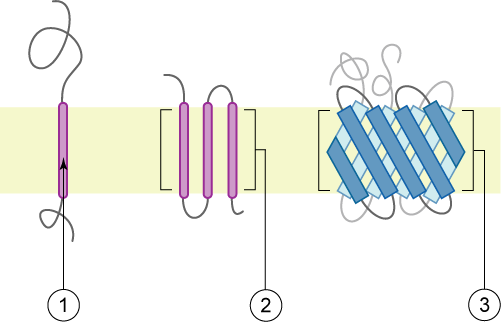
\includegraphics[width = 0.5\textwidth]{figs/mb.png}
\caption{Diferentes topologías de proteínas transmembrana.}
\end{figure}

El PDBTM (Protein Data Bank of Transmembrane Proteins) es una selección completa y actualizada de proteínas transmembrana. A fecha de septiembre de 2022, contiene más de 7600 proteínas transmembrana, el 92,6\% de ellas con elementos TM de hélices alfa. Este número de proteínas TM es relativamente bajo, en comparación con las más de 160.000 estructuras del PDB, ya que las proteínas TM suelen ser más difíciles de purificar y las condiciones de cristalización a menudo son difíciles de alcanzar. Así pues, aunque difíciles, las predicciones precisas de los motivos TM y de la topología general de la proteína pueden ser esenciales para definir la arquitectura de la proteína e identificar dominios que podrían estudiarse estructural o funcionalmente de forma independiente.

\begin{figure}[h]
\centering
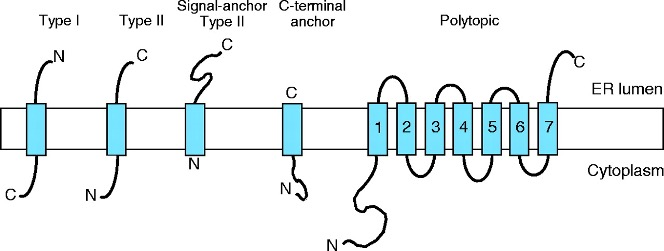
\includegraphics[width = 0.8\textwidth]{figs/alphaTM.jpg}
\caption{Diferentes topologías de hélices transmembrana.}
\end{figure}

Los protocolos actuales de predicción transmembrana muestran una precisión del 90\% en la definición de los elementos TM, pero sólo del 80\% en lo que respecta a la topología de la proteína. Sin embargo, algunos autores afirman que en algunos tipos de proteínas, la precisión no supera el 70\%, debido a los pequeños conjuntos de datos de proteínas TM. Los métodos más recientes, basados en deep-learning parecen haber aumentado la precisión a valores cercanos al 90\% para varios grupos de proteínas.

\section{Subcellular localization tags and post-translational modification sites}
Muchas funciones celulares están compartimentadas en el núcleo, las mitocondrias, el retículo endoplasmático (RE) u otros orgánulos. Por lo tanto, muchas proteínas deben localizarse en esos compartimentos. Eso se consigue mediante la presencia de algunas etiquetas, en forma de secuencias peptídicas cortas que regulan el tráfico y la compartimentación de las proteínas dentro de las células. Normalmente, las señales N-terminales dirigen las proteínas hacia la matriz mitocondrial, el RE o los peroxisomas, mientras que el tráfico hacia el núcleo está regulado por señales de localización nuclear (NLS) y señales de exportación nuclear (NES). Estos motivos cortos son difíciles de predecir, ya que los conjuntos de datos de señales validadas son pequeños. El uso de secuencias consenso permitió realizar predicciones, aunque en muchos casos con un alto nivel de incertidumbre. Como ya puede sospechar, en la última década han aparecido un montón de nuevos métodos basados en el aprendizaje profundo. Si te interesa este tema, consulta la reciente revisión del laboratorio Pollastri.

Las modificaciones postraduccionales a menudo se producen en patrones específicos que incluyen residuos importantes para procesos como la fosforilación o la ubiquitinación. También en este caso, el uso de métodos de aprendizaje profundo para predecir estas modificaciones puede ayudar a identificarlas con precisión y rapidez.


%14/02 - Modesto
\chapter{Modelado por homología avanzado}
\section{Del modelado homológico al threading}
\subsection{Métodos de threading o reconocimiento de pliegues}
Como ya se ha mencionado, la introducción de perfiles basados en HMM durante la primera década de este siglo condujo a una gran mejora en la detección de plantillas y el modelado de proteínas en la zona crepuscular, es decir, proteínas con sólo homólogos distantes (<25-30\% de identidad) en las bases de datos. Con el fin de explotar la potencia de las búsquedas HMM, esos métodos evolucionaron de forma natural hacia métodos iterativos de threading, basados en la construcción de modelos multiplantilla, implementados en I-TASSER, Phyre2 y RosettaCM, entre otros. Estos métodos suelen denominarse \textbf{métodos de Threading o de reconocimiento de pliegues}. Nótese que la clasificación de los métodos de modelado suele ser borrosa. La versión actual de SwissModel y el uso de HHPred+Modeller ya se basan en perfiles HMM para la identificación y alineación de plantillas, por lo que también son estrictamente métodos de reconocimiento de pliegues.

Ambos términos pueden utilizarse a menudo indistintamente, aunque algunos autores consideran que el \textbf{reconocimiento de pliegues} es cualquier técnica que utiliza información estructural además de la información de secuencia para identificar homologías remotas, mientras que el \textbf{threading} se referiría a un proceso más complejo de modelado que incluye homologías remotas y también el modelado de interacciones de aminoácidos por pares en la estructura. Por lo tanto, HHPRED es un método de reconocimiento de pliegues y su uso junto con Modeller, podría considerarse de hecho threading.

\begin{figure}[h]
\centering
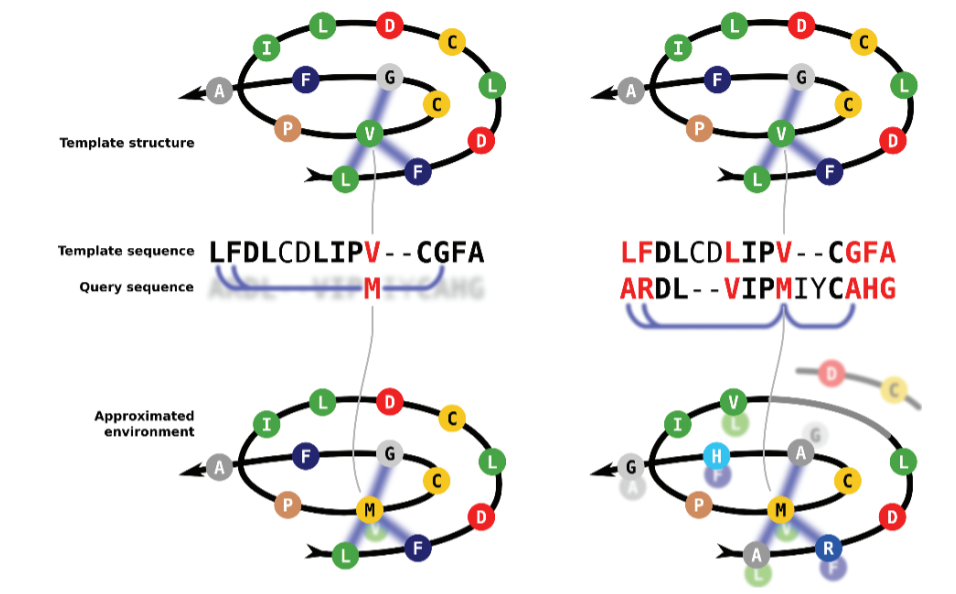
\includegraphics[width = 0.7\textwidth]{figs/fr.png}
\caption{La idea que subyace al reconocimiento de pliegues es que, en lugar de comparar secuencias, pretendemos comparar estructuras. En la aproximación Frozen (izquierda), se alinea un residuo con la estructura de la plantilla (un punto de anclaje) y luego se evalúa la probabilidad de que los residuos cercanos en la secuencia de consulta estén en la misma posición que el equivalente en la plantilla. Por otro lado, los métodos Defrost utilizan perfiles para generar alineaciones mejoradas que permiten mejores puntos de partida para los cálculos de energía durante los pasos iterativos de modelado; tienen varios puntos de anclaje y permiten una estructura más flexible. }
\end{figure}

Iterative Threading ASSembly Refinement (I-TASSER) es uno de los métodos y servidores de threading más utilizados. Este método fue clasificado como el servidor número 1 para la predicción de la estructura de proteínas en los experimentos CASP7, CASP8, CASP9, CASP10, CASP11, CASP12, CASP13 y CASP14 de toda la comunidad. I-TASSER genera en primer lugar modelos atómicos tridimensionales (3D) a partir de múltiples alineaciones de threading y simulaciones iterativas de ensamblaje estructural que se seleccionan y mejoran de forma iterativa. La calidad de las alineaciones de plantilla (y, por tanto, la dificultad de modelar los objetivos) se juzga en función de la importancia estadística de la mejor alineación de roscado, es decir, la \textbf{puntuación Z}, que se define como la puntuación de energía en unidades de desviación estándar en relación con la media estadística de todas las alineaciones.

\begin{figure}[h]
\centering
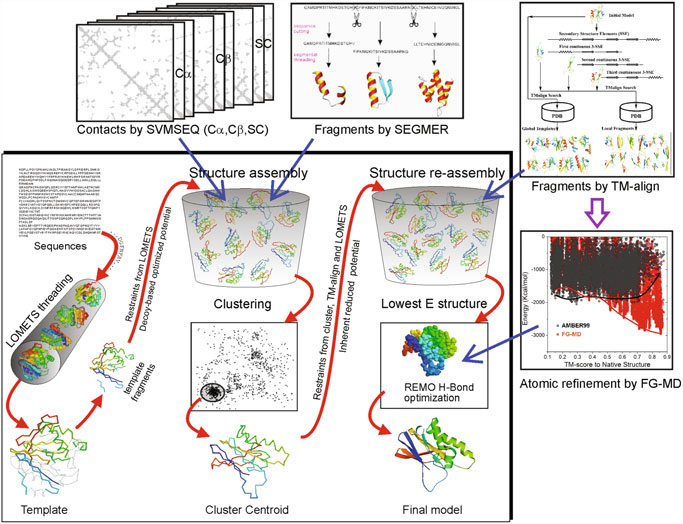
\includegraphics[width = 0.6\textwidth]{figs/paste-29011FF5.png}
\caption{Diagrama de flujo del modelado de estructuras proteicas I-TASSER.}
\end{figure}

En primer lugar, I-TASSER utiliza Psi-BLAST contra bases de datos curadas para seleccionar secuencias homólogas y generar un perfil de secuencia. Ese perfil se utiliza para predecir la estructura secundaria y generar múltiples modelos fragmentados utilizando varios programas. A continuación, se seleccionan los mejores modelos de cada programa para las siguientes etapas. En la segunda etapa, los fragmentos continuos en las alineaciones de roscado se extirpan de las estructuras de plantilla y se utilizan para ensamblar conformaciones estructurales de las secciones que se alinearon bien, con las regiones no alineadas (principalmente bucles/colas) construidas mediante modelado \textit{ab initio}. El ensamblaje de los fragmentos se lleva a cabo mediante una técnica de simulación aleatoria Monte Carlo de intercambio de réplicas modificada, que implementa varias simulaciones de réplicas en paralelo utilizando diferentes condiciones que se intercambian periódicamente. Estas simulaciones tienen en cuenta múltiples parámetros, como las estadísticas del modelo (valores atípicos estereoquímicos, enlaces H, hidrofobicidad...), restricciones espaciales y predicciones de contacto entre pares de aminoácidos. En cada paso, los modelos de salida se agrupan para seleccionar los representativos para la siguiente etapa. Un último paso de refinamiento incluye el modelado de rotámeros y el filtrado de choques estéricos.

Algo interesante de I-TASSER es que está integrado dentro de un servidor con muchas otras aplicaciones, incluyendo algunas de las herramientas que utiliza I-TASSER y otros métodos avanzados basados en I-TASSER, como I-TASSER-MTD para proteínas grandes y multidominio o C-I-TASSER que implementa un paso de aprendizaje profundo, similar a Alphafold2.

\begin{figure}[h]
\centering
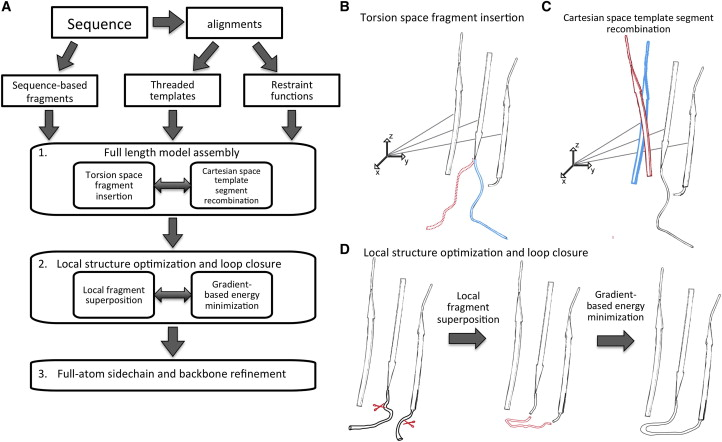
\includegraphics[width = 0.6\textwidth]{figs/rosettaCM.jpg}
\caption{Protocolo RosettaCM. (A) Diagrama de flujo del protocolo RosettaCM. (B-D) Muestreo conformacional de RosettaCM.}
\end{figure}

RosettaCM es un algoritmo avanzado de modelado homológico o threading del laboratorio Baker, implementado en el software Rosetta y en el servidor web Robetta. RossetaCM proporciona modelos precisos dividiendo la secuencia en fragmentos que se alinean con un conjunto de plantillas seleccionadas, generando modelos precisos mediante un proceso de enhebrado que utiliza diferentes fragmentos de cada una de las plantillas. Además, utiliza un plegamiento \textit{ab initio} menor para rellenar los residuos que no se pudieron asignar durante el enhebrado. A continuación, el modelo se cierra mediante pasos de optimización iterativos que incluyen el muestreo Monte Carlo. Por último, se realiza un refinamiento de todos los átomos hacia un mínimo de energía libre.

\begin{table}[htbp]
\begin{mdframed}[backgroundcolor=black!10]
\centering
\textbf{Nomenclatura: ¿Modelado comparativo, por homología o \textit{ab initio}?} 
El modelado \textit{de novo} o \textit{ab initio} solía significar modelar una proteína sin utilizar una plantilla. Sin embargo, esta definición estricta se desdibuja en la década de 2000 gracias a métodos avanzados que utilizan fragmentos. Protocolos de hilado como RosettaCM e I-Tasser, entre otros, utilizan fragmentos que pueden proceder o no de estructuras proteicas homólogas. Por lo tanto, no pueden clasificarse como modelización homológica, pero a veces se denominan métodos comparativos o híbridos.
\end{mdframed}
\end{table}

\subsection{Funciones de puntuación en el modelado de proteínas mediante threading y aprendizaje profundo}
En el modelado de proteínas, se utilizan varias funciones de puntuación para evaluar la similitud de las estructuras proteicas. La desviación media cuadrática (\textbf{RMSD}) mide la similitud tridimensional calculando la RMSD de las coordenadas atómicas C$\alpha$ tras la alineación estructural. Sin embargo, es sensible a los valores atípicos y puede pasar por alto buenos modelos. \textbf{TM-Score} es una alternativa normalizada a RMSD, que va de 0 a 1, que tiene en cuenta la longitud de la proteína y está menos influenciada por los valores atípicos.

En CASP, la puntuación de los modelos se basa en la Prueba de Distancia Global (\textbf{GDT}), a menudo expresada como un porcentaje entre 0 y 100, que mide el número de residuos dentro de un corte de distancia establecido. En concreto, la \textbf{GDT-TS} calcula la GDT media para los límites de 1, 2, 4 y 8 $\AA$. Al igual que la RMSD, la puntuación GDT depende de la longitud, ya que su puntuación media para pares de estructuras aleatorias sigue una ley de potencia que depende del tamaño de la proteína. Para solucionar este problema, la puntuación Z de GDT-TS, utilizada en RosettaCM, indica la calidad y dispersión de los datos basándose en los valores de la media y la desviación estándar. Este uso de la puntuación Z o de las puntuaciones estándar es habitual en matemáticas, ya que refleja cuántas desviaciones estándar hay entre una puntuación bruta y la media.

Por último, el plDDT, o \textbf{lDDT} estimado por residuo utilizado en AlphaFold y métodos relacionados, proporciona una puntuación normalizada por residuo de la distancia libre de superposición C$\alpha$-atómica, con valores que van de 0 a 100. Esta puntuación puede referirse a una sola estructura o a un conjunto, ofreciendo información detallada sobre la precisión del modelado de proteínas. Además, si una región de la proteína es naturalmente muy flexible o intrínsecamente desordenada, en cuyo caso no tiene ninguna estructura bien definida, también tendrá una lDDT más baja.

\section{De los mapas de contactos a los mapas de características de alta resolución por pares}
Un mapa de contactos de proteínas ilustra las interacciones entre todos los pares posibles de residuos de aminoácidos en la estructura tridimensional de una proteína. Se muestra como una matriz binaria con n filas y columnas, donde n representa el número de residuos de la secuencia. En esta matriz, el elemento en la posición ij se marca como 1 si los residuos i y j están en contacto dentro de la estructura. El contacto suele definirse como la proximidad de los residuos por encima de un determinado umbral de distancia, que en los ejemplos de la figura \ref{fig:contact} es de 9 $\AA$. Los patrones de estos mapas ponen de relieve las diferencias entre motivos y reflejan los tramos de estructura secundaria.

\begin{figure}[h]
\centering
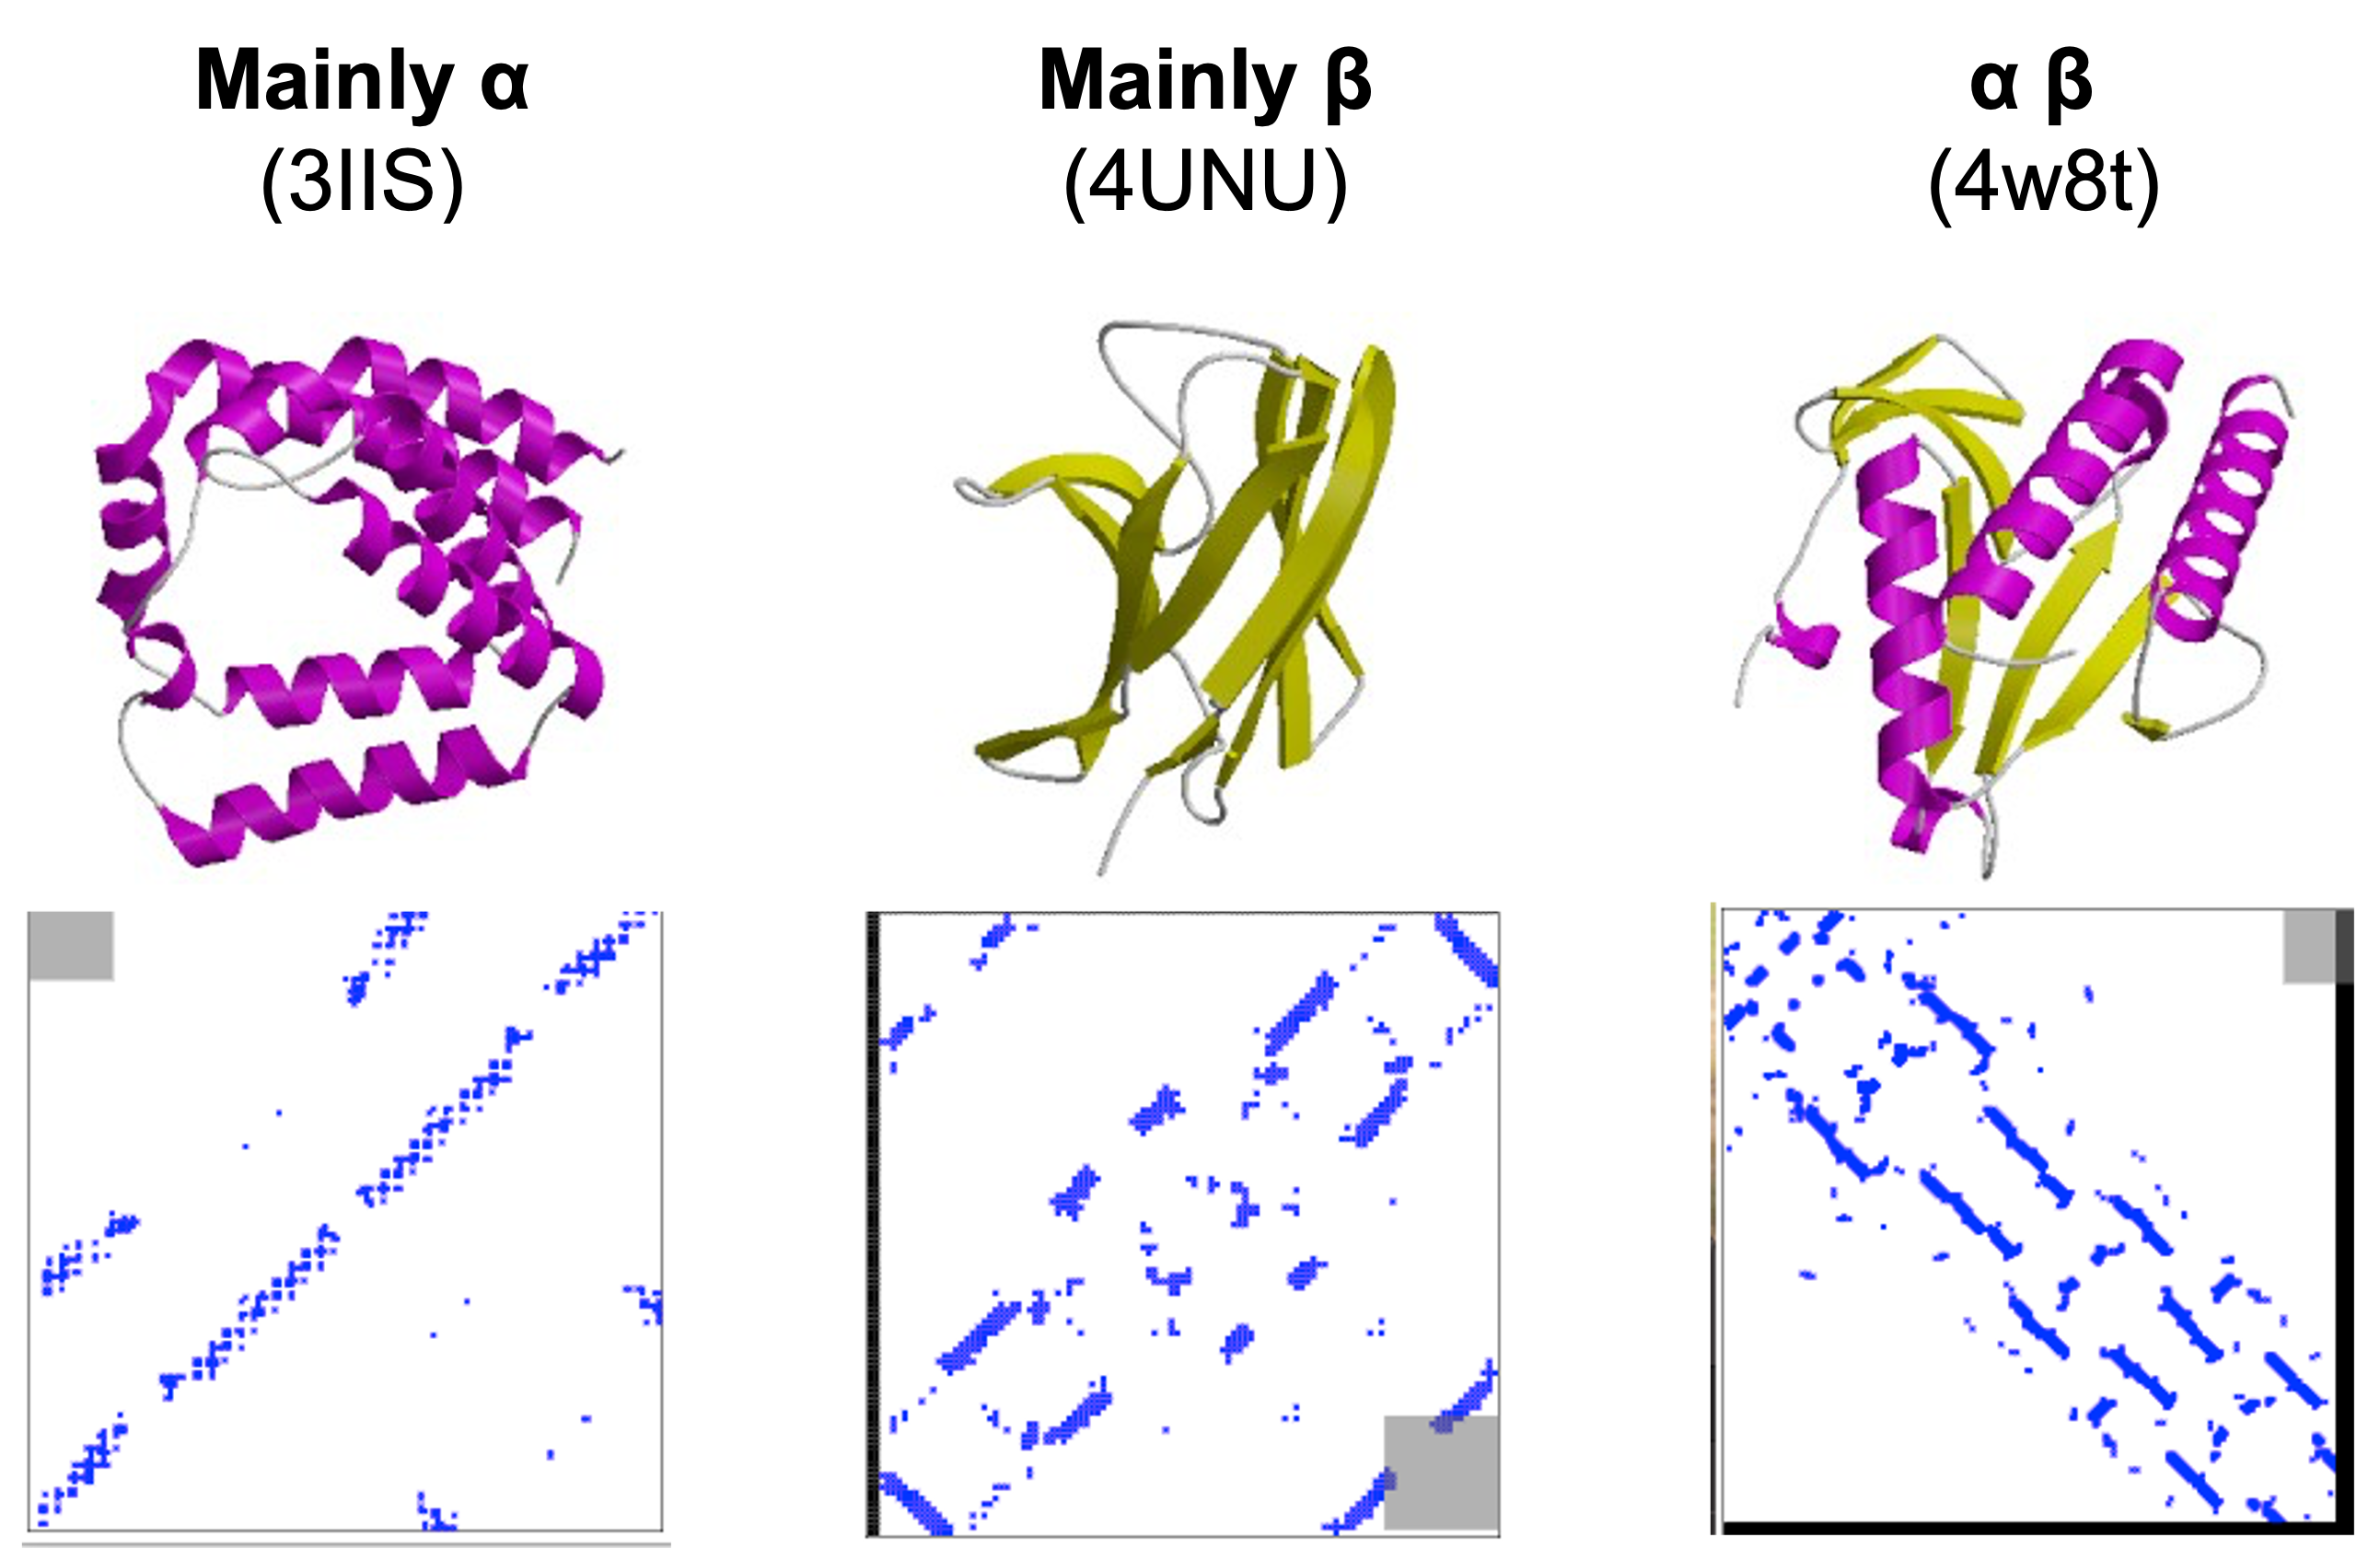
\includegraphics[width = 0.6\textwidth]{figs/contact.png}
\caption{Mapa basado en contactos de proteínas representativas. El mapa representa una matriz de posiciones de aminoácidos en las secuencias de proteínas (tanto en el eje X como en el Y); los contactos se indican con puntos azules. Cuando varios residuos consecutivos de la secuencia interactúan, los puntos forman tramos diagonales.}
\label{fig:contact}
\end{figure}

Para determinar el pliegue de una proteína basta con disponer de información precisa sobre los contactos entre residuos y residuos. Sin embargo, el uso de estos mapas en el modelado de proteínas supone un reto, ya que la predicción de estos contactos no es sencilla. La llegada del análisis de acoplamiento directo (\textbf{DCA}), que extrae la coevolución de residuos de alineaciones de secuencias múltiples (MSA) como se muestra en la Figura \ref{fig:contact-evol}, ha mejorado las predicciones de los mapas de contactos. Esto ha facilitado su uso en el plegamiento de proteínas con métodos como PSICOV y Gremlin. Sin embargo, en el caso de las proteínas con pocas secuencias homólogas, los contactos predichos suelen ser de baja calidad, lo que dificulta el modelado preciso de proteínas asistido por contactos.

\begin{figure}[h]
\centering
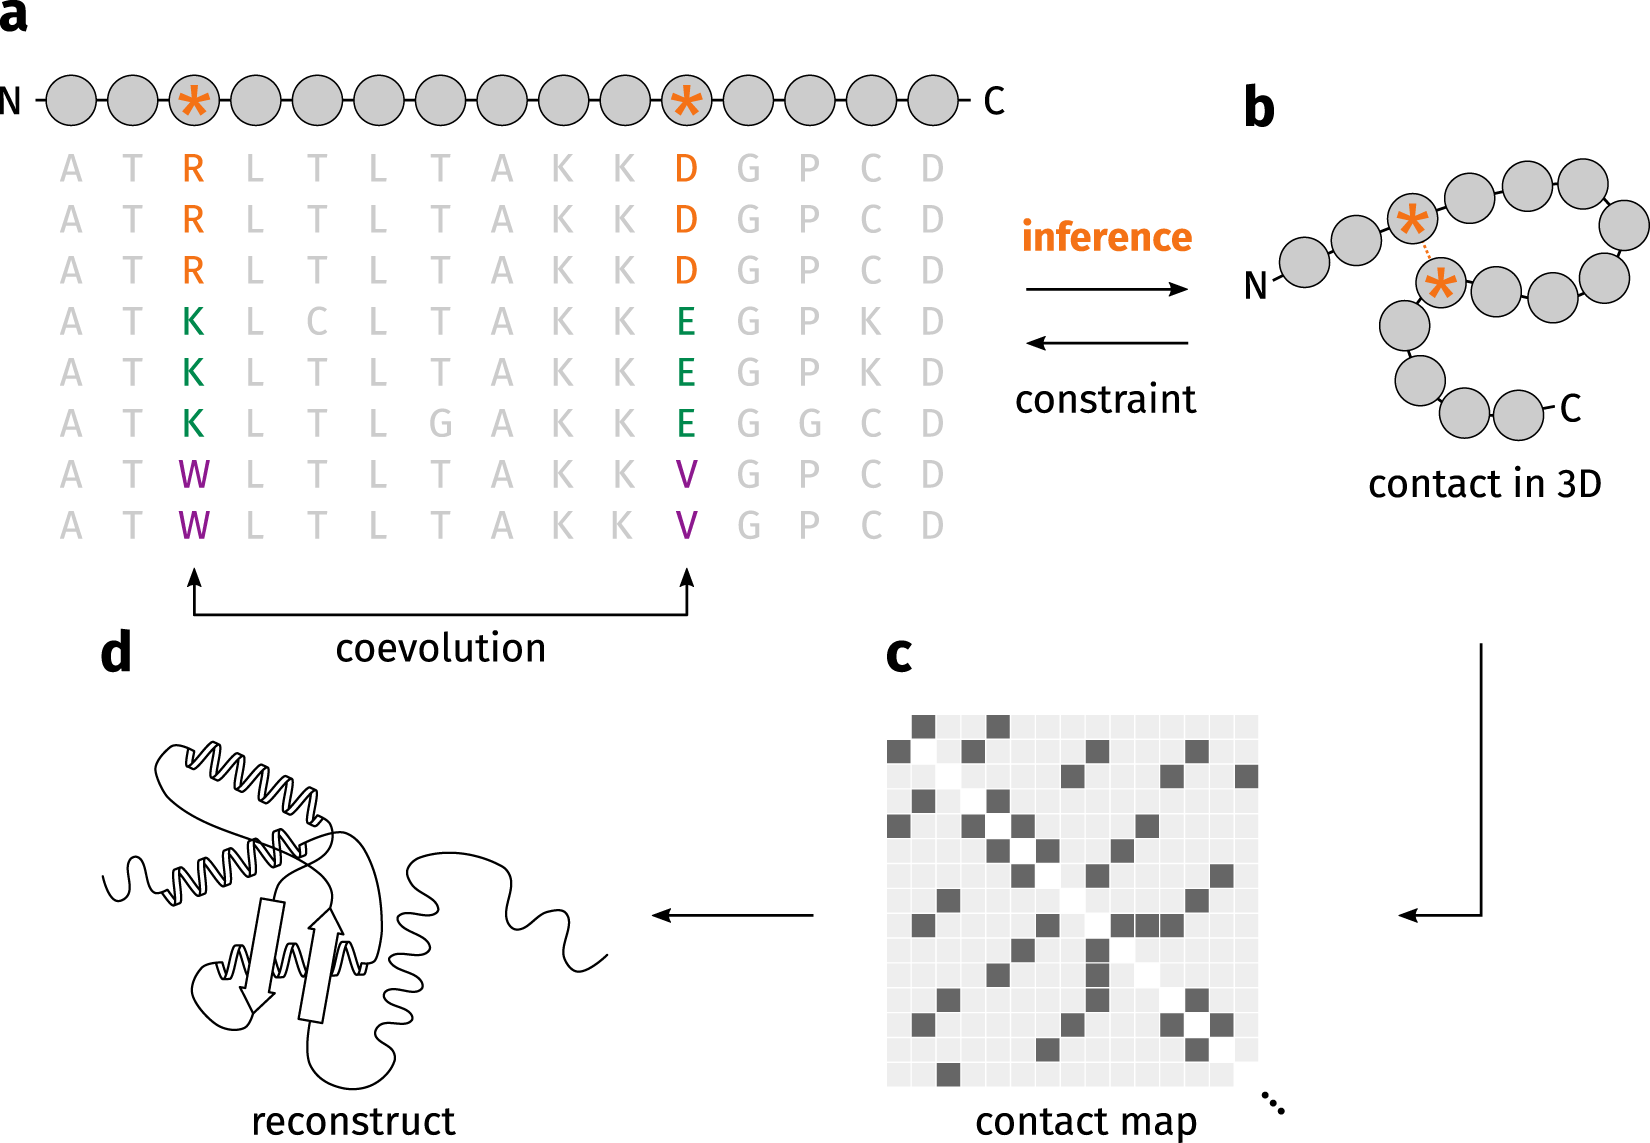
\includegraphics[width = 0.6\textwidth]{figs/contact_evol.png}
\caption{Esquema de cómo los métodos de coevolución extraen información sobre la estructura de las proteínas a partir de un alineamiento múltiple de secuencias (MSA).}
\label{fig:contact-evol}
\end{figure}

\subsection{Implementación de varias capas de información procesada por métodos de redes neuronales y aprendizaje profundo}
El aprendizaje profundo es un subcampo del aprendizaje automático basado en redes neuronales artificiales (NN). Las redes neuronales se introdujeron inicialmente a finales de las décadas de 1940 y 1950, pero volvieron a cobrar importancia en la década de 2000 con el aumento de la capacidad de cálculo y el uso de GPU. En esencia, una NN utiliza múltiples capas interconectadas para transformar diversos datos de entrada, como MSA y mapas de contacto de alta resolución, en características complejas que pueden predecir resultados complejos, como la estructura tridimensional de una proteína. Las NN pretenden simular el comportamiento del cerebro humano, procesando grandes cantidades de datos y aprendiendo de ellos. El aprendizaje profundo utiliza NN de múltiples capas para optimizar y refinar la precisión.

\begin{figure}[h]
\centering
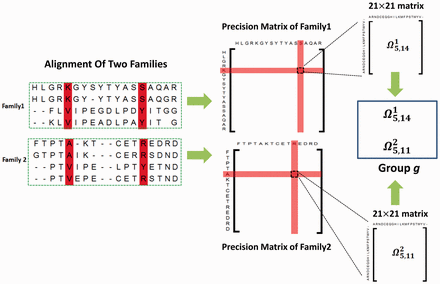
\includegraphics[width = 0.8\textwidth]{figs/contact2.png}
\caption{Ilustración de la agrupación de pares de columnas y submatrices de precisión para la predicción avanzada de mapas de contactos. En el ejemplo, las columnas 5 y 14 de la primera familia están alineadas con las columnas 5 y 11 de la segunda familia, respectivamente, por lo que el par de columnas (5,14) de la primera familia y el par (5,11) de la segunda familia se asignan al mismo grupo. En consecuencia, las dos submatrices de precisión se asignarán al mismo grupo.}
\label{fig:contact2}
\end{figure}

El siguiente nivel de complejidad en los mapas de contactos implica su aplicación a proteínas relacionadas a distancia mediante la comparación de conjuntos de DCA de diferentes familias de proteínas, lo que a veces se denomina análisis de acoplamiento evolutivo conjunto (Figura \ref{fig:contact2}). Este método requiere procesar cantidades masivas de información, lo que aumenta las demandas computacionales. Por lo tanto, el uso de redes neuronales entrenadas y métodos avanzados de aprendizaje profundo ha mejorado significativamente las capacidades de modelado de proteínas.

En este contexto, la introducción de métodos supervisados de aprendizaje automático que predicen contactos ha superado a los métodos DCA mediante el empleo de redes neuronales multicapa. Estos métodos incorporan mapas de contactos de alta resolución (Figura \ref{fig:highresmaps}), que contienen información enriquecida que incluye no solo contactos, sino también distancias y ángulos, representados en una escala de probabilidad similar a un mapa de calor.

\begin{figure}[h]
\centering
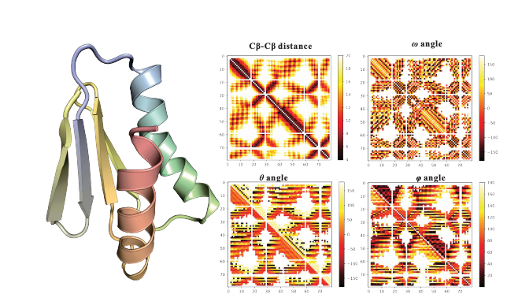
\includegraphics[width = 0.8\textwidth]{figs/high_res_maps.png}
\caption{Ejemplo de mapas de contacto de alta resolución de 6MSP.}
\label{fig:highresmaps}
\end{figure}
%19/02 - Modesto
\chapter{Modelado de proteínas en la era de Alphafold}
\section{La historia del modelado de estructuras de proteínas contada por un concurso (CASP)}
Cada dos años, desde 1994, grupos del campo de la bioinformática estructural llevan a cabo un experimento mundial en el que predicen un conjunto de estructuras proteicas desconocidas en una competición controlada, similar a una prueba a ciegas, y comparan sus resultados con las estructuras obtenidas experimentalmente. Se trata del CASP (Critical assessment of Protein Structure Prediction).

Los mejores grupos de investigación del sector ponen a prueba sus nuevos métodos y protocolos en el CASP. Sin embargo, en el CASP13 (2018), una empresa de IA llamada Deepmind (filial de Google) entró en escena. Su método, llamado Alphafold ganó claramente el CASP13. Alphafold (v.1) implementó mejoras en algunos enfoques utilizados recientemente y creó un proceso completamente nuevo. En lugar de crear mapas de contactos a partir del alineamiento y luego plegar la estructura, utilizaron una unidad MRF (Markov Random Field) para extraer las características principales de la secuencia y el MSA por adelantado y procesar toda esta información en una red neuronal multicapa (llamada ResNet) que también predijo probabilidades de distancia en lugar de contactos, lo que dio como resultado una gran precisión. A continuación, Alphafold utiliza toda la información posiblemente obtenida para crear la estructura y luego mejorarla mediante la minimización de la energía (método de descenso más pronunciado) y la sustitución de porciones con una base de datos seleccionada de fragmentos de proteínas.

\begin{figure}[h]
\centering
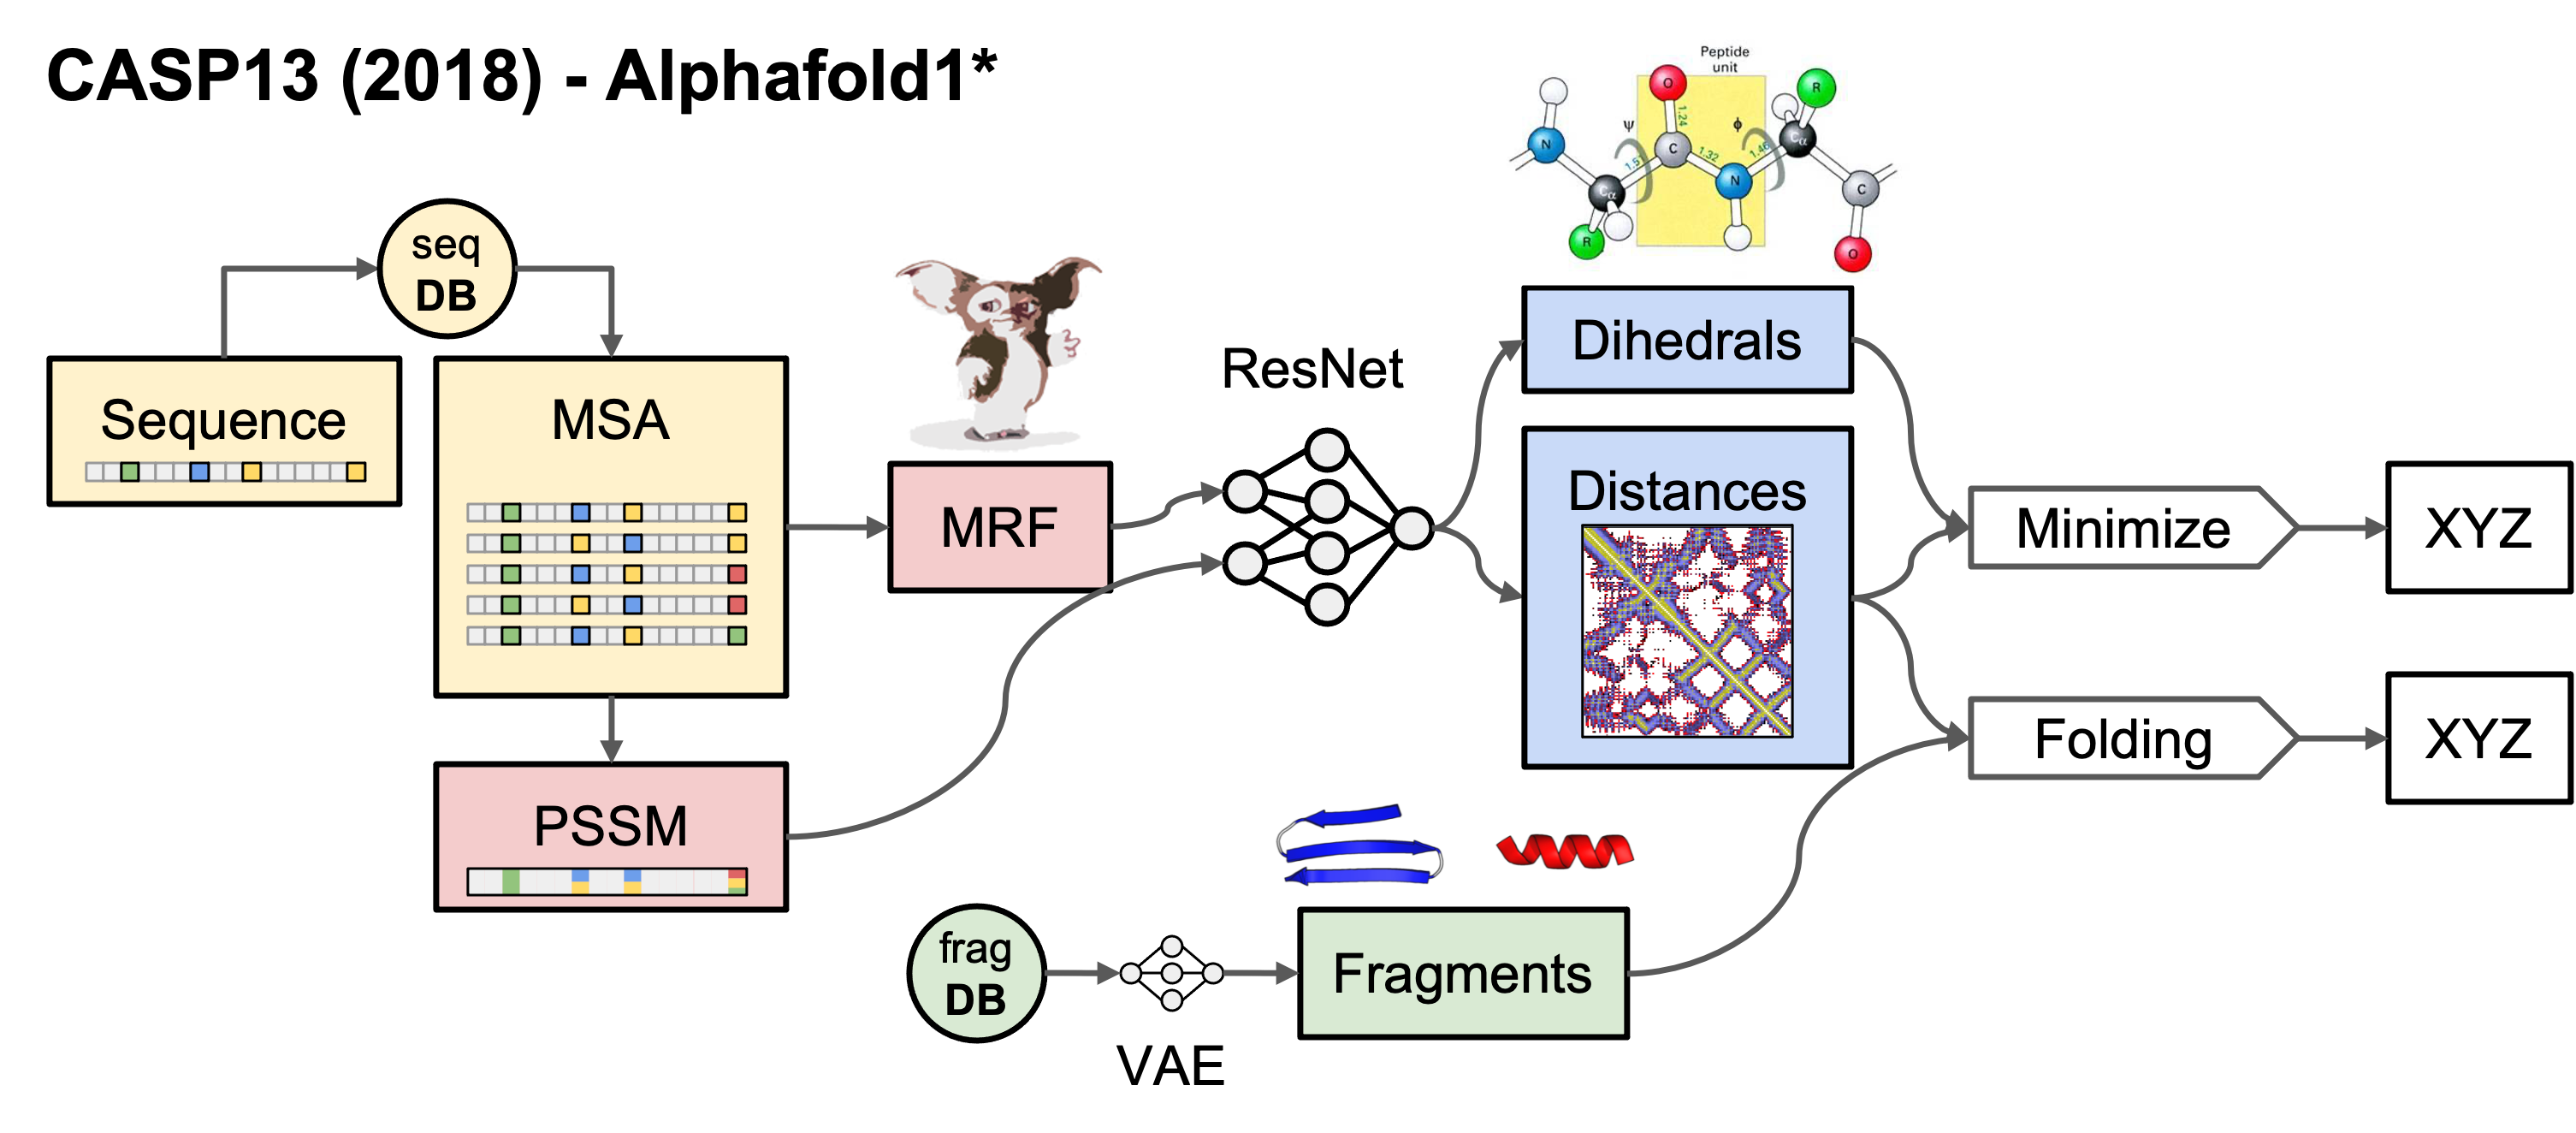
\includegraphics[width = 0.8\textwidth]{figs/alphafold1.png}
\caption{Flujo de trabajo del primer método Alphafold presentado en CASP13. MSA significa alineación múltiple de secuencias; PSSM indica Position-specific-scoring matrix y MRF significa Markov Random Field (o modelo Potts).}
\end{figure}

Después de Alphafold, también se desarrollaron métodos similares y se pusieron a disposición del público en general, como el trRosetta, del laboratorio Baker, disponible en el software de código abierto Rosetta y en el servidor Robetta. Esto llevó a cierta controversia (sobre todo en Twitter) sobre el acceso abierto al software CASP y más tarde DeepMind publica todo el código en GitHub.

\section{CASP14 o cuando la predicción de la estructura de las proteínas alcanza la mayoría de edad para los biólogos (no estructurales)}
Había mucho revuelo en CASP14 y los chicos de DeepMind no decepcionaron a nadie. Alphafold2 dejó muy atrás a todos sus competidores, tanto en términos relativos (puntuación frente a los demás grupos) como en términos absolutos (RMSD alfa-carbono más bajo). Como se ha destacado anteriormente, la precisión de muchas de las estructuras predichas estaba dentro del margen de error de los métodos de determinación experimental.

\begin{figure}[h]
\centering
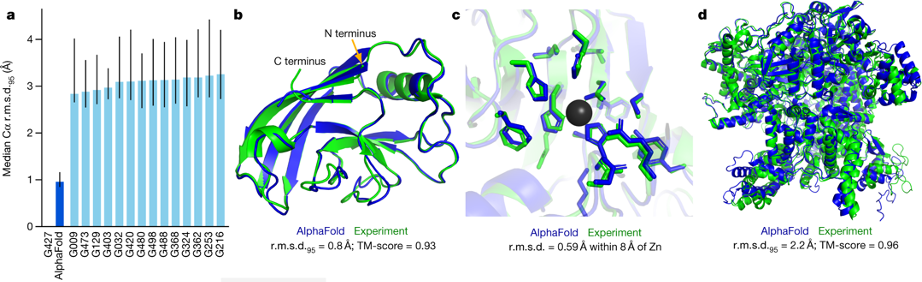
\includegraphics[width = 0.8\textwidth]{figs/jumper2021.png}
\caption{Rendimiento de Alphafold2 en el conjunto de datos CASP14 en relación con las 15 mejores entradas. Los datos son la mediana y el intervalo de confianza del 95\% de la mediana, para RMSD alfa-carbono. Los paneles b-c-d muestran ejemplos de comparación entre el modelo y las estructuras experimentales.}
\end{figure}

Deepming tardó algún tiempo (ocho meses, lo que hoy en día es una eternidad) en publicar el método y liberar el código en Github, pero otros métodos nuevos, como RoseTTAfold y C-I-Tasser fueron capaces de obtener resultados similares y estaban disponibles en servidores públicos, lo que quizá empujó a Deepmind a ponerlo todo a disposición de la comunidad científica. No es de extrañar que un grupo de científicos independientes (Sergey Ovchinnikov, Milot Mirdita y Martin Steinegger) decidieran implementar Alphafold2 en un cuaderno Colab, llamado ColabFold, que está disponible gratuitamente en línea a través de la plataforma de cuadernos Colab de Google. Otras implementaciones libres de Alphafold han estado y están disponibles, pero ColabFold ha sido la más ampliamente discutida y conocida. Implementaron algunos trucos para acelerar el modelado, sobre todo el uso de MMSeqs2 (desarrollado por el grupo de Martin Steinegger) para buscar estructuras homólogas en Uniref30, lo que convirtió a Colabfold en un método rápido que hizo casi inútiles todos los métodos avanzados anteriores. Este fue el verdadero avance en el campo de la predicción de estructuras de proteínas, haciendo accesible Alphafold y, también muy importante, facilitó el desarrollo posterior del método, implementando muy rápidamente nuevas características, como la predicción de complejos de proteínas, que de hecho se mencionó por primera vez en Twitter y luego dio lugar a varios nuevos métodos dedicados, incluyendo AlphaFold-multimer de Deepmind o AlphaPullDown.

\section{Alphafold como paradigma de una nueva era}
\subsection{¿Por qué Alphafold es tan preciso?}
La filosofía detrás de Alphafold v.2 (a partir de ahora, sólo Alphafold) y métodos relacionados es tratar el problema del plegamiento de proteínas como un problema de aprendizaje automático, similar al procesamiento de imágenes. En todos estos problemas, la entrada al modelo de aprendizaje profundo es un volumen (tensor 3D). En el caso de la visión por ordenador, las imágenes 2D se expanden como volúmenes debido a los canales RGB o HSV. Del mismo modo, en el caso de la predicción de distancias, las características 1D y 2D predichas se transforman y empaquetan en un volumen 3D con muchos canales de información entre residuos.

\begin{figure}[h]
\centering
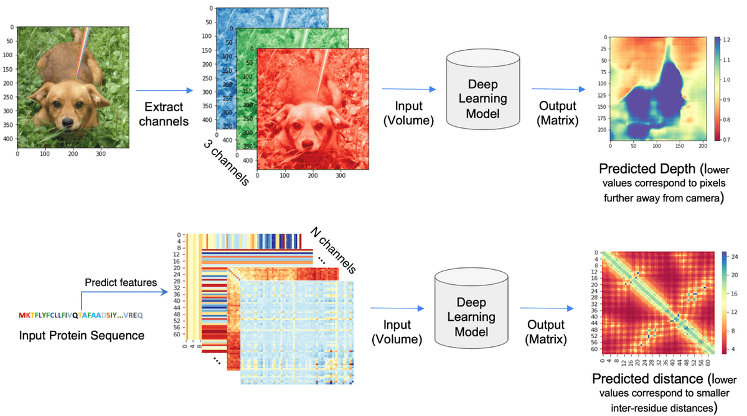
\includegraphics[width = 0.8\textwidth]{figs/machine_fold.png}
\caption{Desde la perspectiva del desarrollo de métodos de Deep Learning, el problema de la predicción del distograma de proteínas o distancia en valor real (fila inferior) es similar al «problema de predicción de profundidad» en visión por ordenador.}
\end{figure}

Alphafold puede explicarse como un pipeline con tres tareas interconectadas (véase la imagen inferior). En primer lugar, a diferencia de Alphafold v.1, la entrada de Alphafold es un MSA «en bruto», es decir, la red de aprendizaje profundo extrae la información coevolutiva directamente del MSA. Consulta varias bases de datos de secuencias de proteínas y construye un MSA que se utiliza para seleccionar plantillas. Esto puede ser un paso limitante que afecte a la velocidad del modelado (véase más adelante), pero también puede estar relacionado con la precisión del modelo, como se ha demostrado recientemente en CASP15.

En la segunda parte del diagrama, AlphaFold toma la alineación de secuencias múltiples y las plantillas, y las procesa en un \textbf{transformador}. Este proceso ha sido denominado por algunos autores como inter-residue interaction map-threading. El objetivo de esta parte es extraer capas de información para generar mapas de interacción de residuos. Un mejor modelo del MSA mejorará la caracterización de la geometría de la red, lo que simultáneamente ayudará a refinar el modelo del MSA. Es importante destacar que, en el AF2 Evoformer, este proceso es iterativo y la información va y viene por toda la red. En cada paso de reciclaje, la complejidad del mapa aumenta y, por tanto, el modelo mejora (el modelo original utiliza 3 ciclos). Como se explica en el post de Carlos Outerial en el sitio OPIG:
\begin{quote}
Esto es más fácil de entender con un ejemplo. Supongamos que observas el alineamiento múltiple de secuencias y notas una correlación entre un par de aminoácidos. Llamémoslos A y B. Usted parte de la hipótesis de que A y B están próximos, y traslada esta suposición a su modelo de la estructura. Posteriormente, examinas dicho modelo y observas que, puesto que A y B están próximos, hay muchas probabilidades de que C y D también lo estén. Esto conduce a otra hipótesis, basada en la estructura, que puede confirmarse buscando correlaciones entre C y D en el MSA. Repitiendo esto varias veces, se puede llegar a comprender bastante bien la estructura.
\end{quote}

La tercera parte del pipeline es el módulo de construcción de la estructura, que utiliza la información de los pasos anteriores para construir un modelo 3D de la estructura de la proteína de la secuencia de consulta. Esta red le dará un modelo único end-to-end, sin ningún paso de optimización de la energía. La construcción del modelo se basa en un nuevo concepto de generación de estructuras 3D, denominado \textbf{IPA (Invariant Point Attention)} y en el uso de una lista curada de ángulos de torsión parametrizados para generar las cadenas laterales. Los intentos anteriores de desarrollar un método de extremo a extremo no tuvieron éxito porque la representación de la estructura no era óptima. Incluso los métodos implementados después de AlphaFold, como RoseTTAFold, utilizan métodos menos eficientes y a menudo predicen muy rápidamente y con precisión las coordenadas de la columna vertebral, pero requieren programas externos para generar un modelo de todos los átomos.

\begin{figure}[h]
\centering
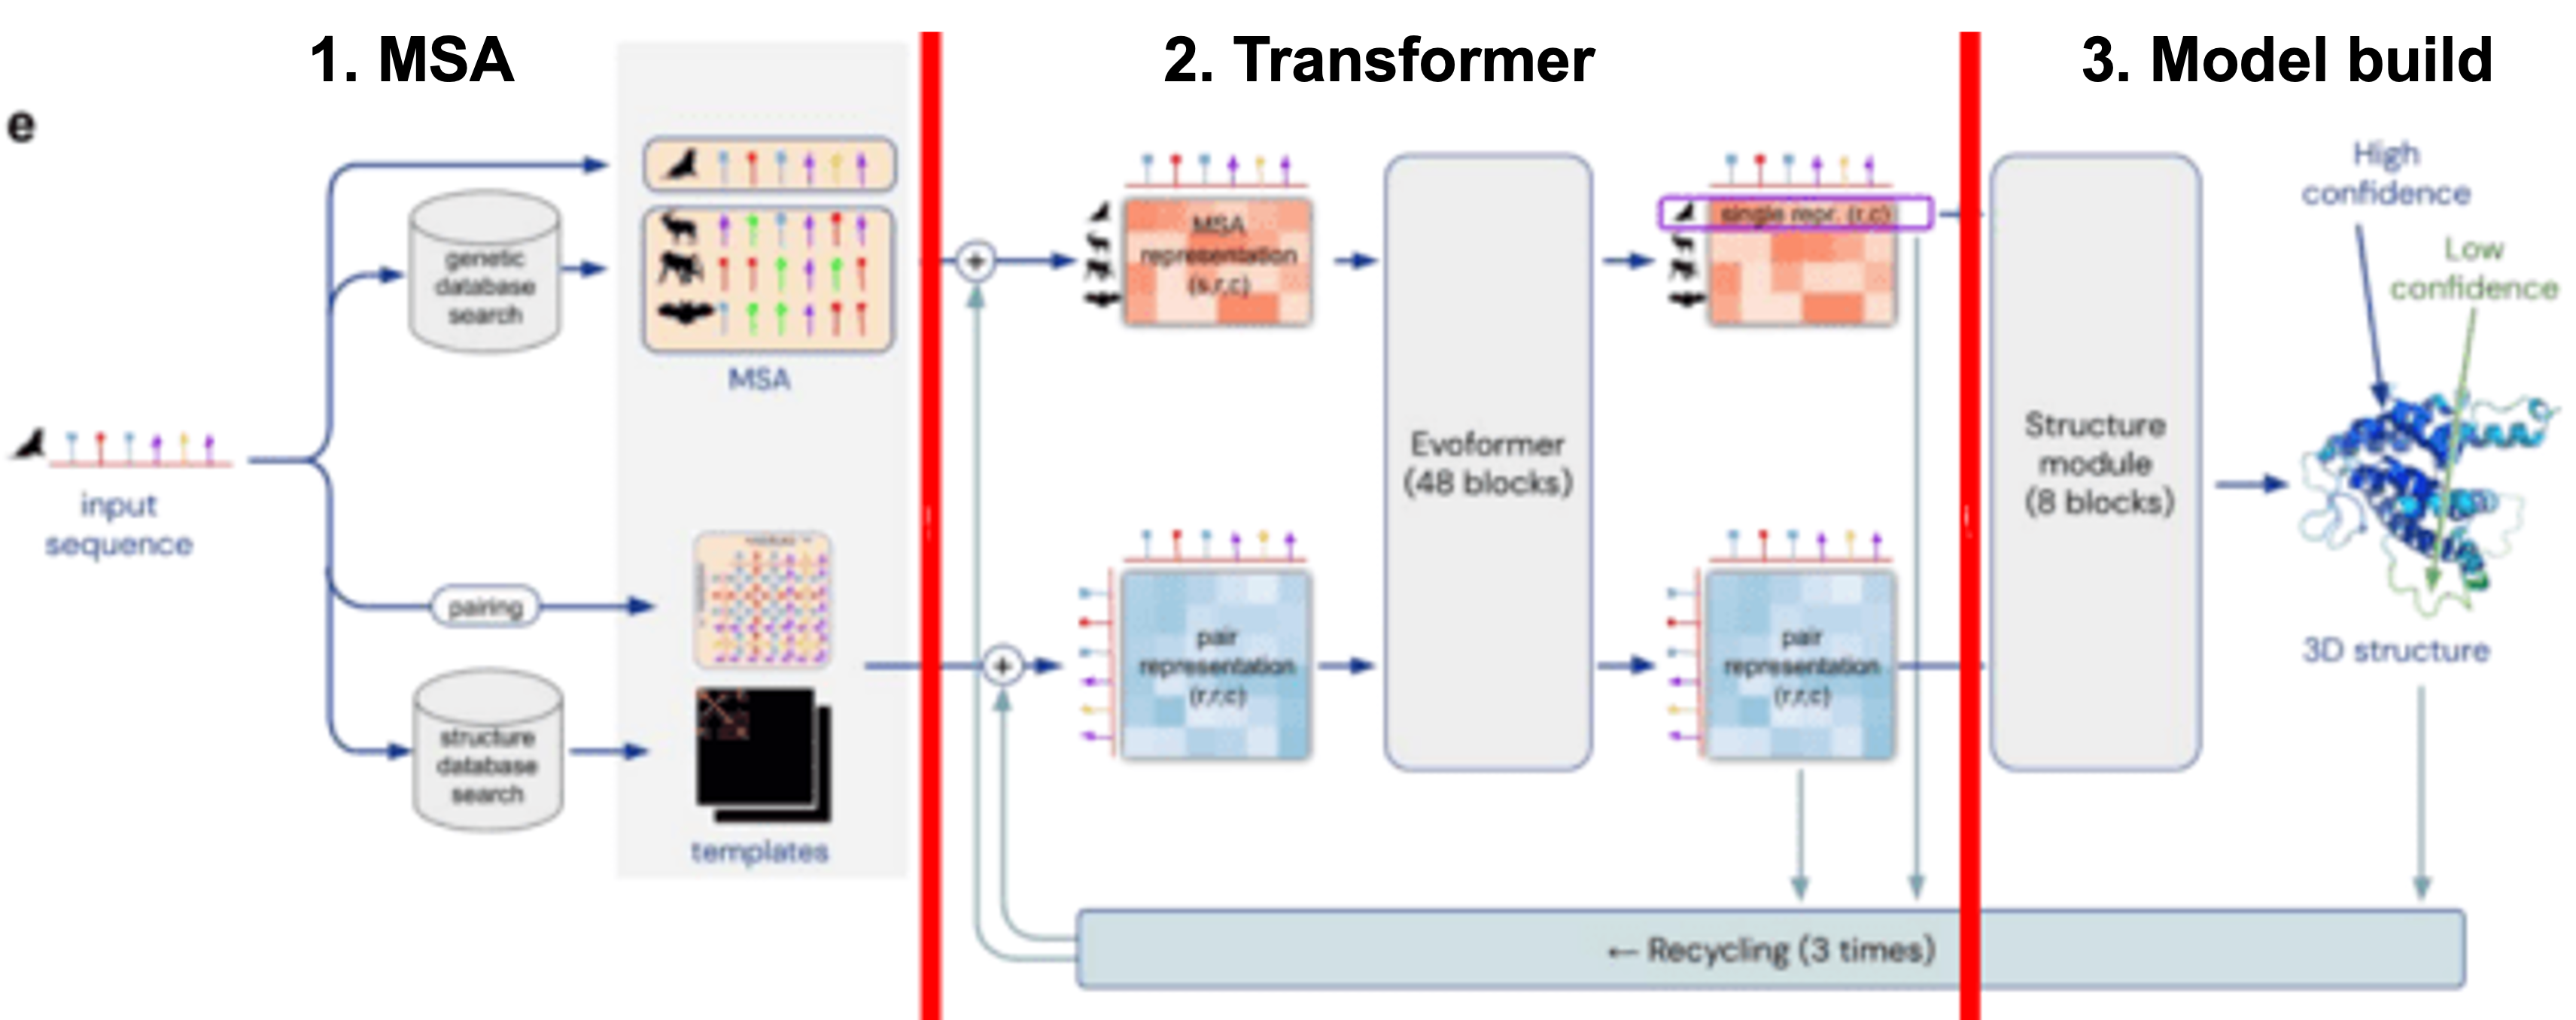
\includegraphics[width = 0.8\textwidth]{figs/alphafold2.png}
\end{figure}

Como para la mayoría de los métodos anteriores, Alphafold dará mejores resultados con proteínas con estructuras relacionadas conocidas y con muchos homólogos en las bases de datos Uniref. Sin embargo, comparado con nada, probablemente dará resultados útiles (limitados) para el llamado «genoma oscuro». Para un trabajo con fagos y elementos móviles bacterianos, secuenciar eso es a menudo frustrante, ya que más del 50\% de las proteínas no tienen homólogos en la base de datos. Así que tenemos un montón de proteínas de función desconocida... Sin embargo, como sabemos que la estructura está más conservada que la secuencia, podemos utilizar la estructura para averiguar la función de nuestras proteínas oscuras. Hay algunos recursos para esto, como los servidores FoldSeek y Dali. Se puede subir el archivo PDB del modelo y buscar estructuras relacionadas en la base de datos RCSB PDB y también en la base de datos Alphafold.

Como ya se ha mencionado, Colabfold pretende agilizar el proceso utilizando MMSeqs en el primer bloque. Además, también se puede adaptar el número de pasos de reciclado. Además, se han desarrollado (y evolucionado) diferentes cuadernos Colabfold para permitir cierta personalización y otras características, como el procesamiento por lotes de múltiples proteínas evitando la recompilación y la identificación de interacciones proteína-proteína.

Los modelos Alphafold pueden evaluarse mediante la \textbf{pLDDT} media, una métrica de confianza por residuo. Se almacena en los campos del factor B de los archivos mmCIF y PDB disponibles para su descarga (aunque a diferencia del factor B, un pLDDT más alto es mejor). La confianza del modelo puede variar mucho a lo largo de una cadena, por lo que es importante consultar la confianza al interpretar las características estructurales. Muy a menudo, los fragmentos de menor confianza no son producto de una mala predicción, sino un indicador de desorden de la proteína.

Otra medida es el PAE (predicted aligned error). Es el error previsto en $\AA$ entre cada par de residuos. Esto no tiene en cuenta ninguna estructura «verdadera», sino que es el error predicho. Así, los bloques de bajo PAE en la matriz PAE muestran que la posición relativa de todos esos residuos es segura, lo que puede mostrar, por ejemplo, que esos residuos forman un dominio bien plegado. pLDDT es un tipo diferente de predicción de error. En lugar de ser la predicción del error por pares entre dos residuos, pLDDT es básicamente «cuánta confianza tengo en la predicción de la posición de cada residuo». En ambos casos, estos valores son devueltos por el modelo de predicción y son estimaciones

Alphafold también se asoció con EMBL-EBI y Uniprot y generó una enorme base de datos curada de proteínas de organismos modelo, la base de datos Alphafold. Esta base de datos aumentó del 48\% al 76\% la fracción del proteoma humano con datos estructurales, y también significa grandes aumentos en el caso de otros organismos modelo, como, incluyendo microorganismos y plantas.

\subsection{¿Ahora qué? La era post-Alphafold}
Como ya se ha mencionado, RoseTTAFold se publicó al mismo tiempo que el artículo y el código de AlphaFold, aunque está claramente inspirado en las capacidades de AlphaFold en CASP14. Se basa en una red de tres pistas, y las implementaciones recientes han permitido predecir interacciones de proteínas con ácidos nucleicos. Otros métodos como AlphaFold y RoseTTAFold se lanzaron posteriormente, al igual que OpenFold y UniFold, que se basan en el marco PyTorch Transformers AI. Más recientemente, RoseTTAFold2, que extiende la arquitectura de tres pistas sobre toda la red e incorpora otros nuevos avances y trucos de AlphaFold, como el FAPE (frame aligned point error) o pasos de reciclado durante el entrenamiento, dando lugar a un modelo de extremo a extremo equivalente en precisión a AF2 para monómeros y AF2-multimer para complejos, con mejor escalado computacional en proteínas y complejos mayores de 1000 residuos.

El uso de MSA se ha citado como una limitación para AlphaFold y métodos relacionados. Sin embargo, las predicciones son significativamente peores sin MSA o con MSA sin profundidad. Una forma de mejorar las predicciones es utilizar un modelo de lenguaje natural de proteínas (PLN), es decir, un modelo entrenado para predecir secuencia a secuencia y que no dependa de buenos MSA. Omegafold y ESMfold (también en Colabfold) son dos nuevas implementaciones que sólo requieren una única secuencia. Son bastante rápidas y funcionan mejor que AlphaFold cuando se utiliza una única secuencia. Sin embargo, dado que PLN se entrena con secuencias existentes, estos métodos obtienen resultados significativamente peores con secuencias huérfanas. Es decir, los modelos lingüísticos parecen limitarse a recordar los MSA de entrenamiento.

La aparición de ESMfold y del Atlas Metagenómico complementario se vio como un nuevo paso que podría desencadenar una nueva revolución en el campo, ya que fue desarrollado por científicos de META. Así que ahora se trataba de una especie de batalla entre Google y Facebook por los métodos de IA más potentes para el modelado de proteínas. Sin embargo, el verano pasado supimos que META había decidido interrumpir el proyecto ESM.

AlphaFold se utilizó de alguna forma en más de la mitad de los protocolos, y aunque el método AlphaFold estándar funcionó mejor que muchos otros métodos, varios grupos lograron mejoras significativas para proteínas monoméricas y ensamblajes de proteínas. En resumen, aprendimos en CASP15 que hay dos formas principales de mejorar AlphaFold: (1) un uso más eficiente de las plantillas, aumentando el tamaño de la base de datos o el muestreo a través de MSA más eficientes, o (2) hackear AlphaFold para utilizar dropouts para generar miles de modelos para cada objetivo, lo que aumenta el tiempo computacional pero también aumenta las posibilidades de obtener mejores modelos. Se han propuesto otras pequeñas mejoras, como pasos de refinamiento o el uso de una búsqueda de plantillas mejorada o nuevas capacidades de puntuación basadas en superficies de Voronoi o Deep Learning.

\subsection{Corolario: ¿Resolvió Deepmind la paradoja de Levinthal?}
El desarrollo de Alphafold y de la base de datos de estructuras Alphafold en colaboración con el EMBL-EBI ha sido el origen de una nueva era. Además, en un nuevo giro, el Atlas Metagenómico de Meta AI descubre prácticamente todo el espacio proteico. Gracias a estos hitos se ha incrementado enormemente la cobertura del espacio de estructuras proteicas, lo que prácticamente cierra la brecha secuencia-estructura. Desde 2020, muchas publicaciones y revistas científicas de todo el mundo publicaron largos artículos sobre el significado de este gran avance en la ciencia y sus aplicaciones en biotecnología y biomedicina y DeepMind afirmó haber resuelto un Gran Desafío de 50 años en bioquímica.

En otras palabras, después de AlphaFold, ¿ya no sería necesario realizar cristalografía de rayos X o resonancia magnética nuclear? En primer lugar, los modelos AlphaFold pueden utilizarse en mapas de densidad electrónica y ayudar a resolver casos complejos. Así, el nuevo marco ayuda a los cristalógrafos a centrar su trabajo en las estructuras más difíciles y sin resolver, como las espirales o las holoproteínas, que provocan modulaciones y desafíos en el desarrollo de los métodos cristalográficos.

Sin embargo, algunos científicos sostienen que Alphafold2 y RoseTTAfold en realidad hacen trampa, ya que no resuelven realmente el problema, sino que generan una vía de aprendizaje profundo que es capaz de eludir el problema. De acuerdo con esto, se ha demostrado que los métodos de aprendizaje automático en realidad no reproducen las rutas de plegamiento esperadas mientras que mejoran las estructuras durante los pasos de reciclaje.

En conclusión, la paradoja de Levinthal no está (todavía) totalmente resuelta, aunque parece estar cerca. Prácticamente, está resuelta para la mayor parte del espacio proteico, pero si una proteína no tiene un homólogo en las bases de datos, todavía quedarán algunas preguntas abiertas.

\subsection{Limitaciones de Alphafold}
Entre las limitaciones se encuentran problemas con complejos de proteínas con otras moléculas como ADN, regiones desordenadas, variantes de splicing alternativo y falta de información evolutiva. El problema del splicing es muy importante en biomedicina. No hay estructuras en PDB de prácticamente ninguna variante de splicing, por lo que no se pueden predecir y puede ser un problema para mutantes específicos de las proteínas o diagnóstico de enfermedades raras. 

Un ejemplo de un target difícil es la proteína Bam35 de un bacteriófago. Se trata de una proteína SSB (single-stranded binding) con un OB-fold. Suelen formar multímeros a la hora de unirse al ADN. Esta proteína tenía unos valores de GMQE mut bajo, con una identidad también reducida. Se crearon tres modelos distintos y se vio que en los tres había una región conservada y una región diversa. La región conservada se utilizó para comparar frente a las bases de datos, pudiendo encontrar casos de similitudes. 

Tras todo esto, en mayo de 2024 llegó Alphafold v3. Ha permitido modelar estructuras de proteínas en relación con otras estructuras como ADN y ARN. Esto es muy importante para el diseño de fármacos. El código está accesible, pero tiene muchas limitaciones. 

%21/02 - Modesto
\section{Alucinación de proteínas y modelos de difusión}
Bioquímicos y químicos llevan décadas soñando con diseñar proteínas con propiedades personalizables. Los primeros diseños de proteínas con éxito se publicaron a finales de los 90 y varios avances del laboratorio de Baker impulsaron la idea. Más recientemente, la inteligencia artificial está iniciando una revolución en este campo que lo cambiará radicalmente para siempre.

Poco después de la publicación de AF2 y RoseTTAFold, se utilizaron para «alucinar» nuevas proteínas. En diciembre de 2021, Baker y sus colegas informaron de la expresión de 129 de estas proteínas alucinadas en bacterias, y descubrieron que alrededor de una quinta parte de ellas se plegaban en algo parecido a su forma predicha. Luego, en 2023, introdujeron RFdiffussion, un nuevo paradigma en el diseño de proteínas, basado en modelos de difusión de IA. Imaginemos que partimos de una nube de átomos colocados al azar (puro ruido). Durante el entrenamiento, los modelos de difusión aplican ruido normalmente aleatorio a una distribución de datos hasta que se asemeja a la estática pura, por ejemplo. A continuación, el modelo aprende a invertir este proceso, generando puntos de datos finales representativos de la distribución de datos original. Este proceso se guía por patrones aprendidos sobre la interacción de átomos y moléculas, lo que permite al modelo «desnaturalizar» la disposición aleatoria inicial y convertirla en un complejo biomolecular realista. El modelo aprende a invertir un «proceso de difusión» en el que el ruido se añade progresivamente a estructuras biomoleculares conocidas. Al aprender a deshacer este proceso, el modelo puede generar nuevas estructuras desde cero.

Más recientemente, varios grupos han combinado modelos de difusión con PNL para desarrollar métodos mejorados de diseño de nuevas proteínas. Las secuencias proteínicas pueden describirse como una concatenación de letras de un alfabeto químicamente definido, los aminoácidos naturales, y, al igual que las lenguas humanas, estas letras se ordenan para formar elementos estructurales secundarios («palabras»), que se ensamblan para formar dominios («frases») que asumen una función («significado»). Una de las similitudes más atractivas es que las secuencias de proteínas, al igual que los lenguajes naturales, son información-completa: almacenan la estructura y la función enteramente en su orden de aminoácidos con una eficiencia extrema. Con los extraordinarios avances en el campo de la PNL para comprender y generar lenguaje con capacidades casi humanas, planteamos la hipótesis de que estos métodos abren una nueva puerta para abordar problemas relacionados con las proteínas a partir únicamente de la secuencia, como el diseño de proteínas.

\section{Alphafold3 amplió el alcance}
Las proteínas están formadas por aminoácidos, pero también incluyen otros componentes. Las holoproteínas suelen contener múltiples cadenas proteicas, iones y cofactores. Además, las funciones de las proteínas suelen implicar interacciones con diversos ligandos, incluidas moléculas de ADN o ARN. Una limitación de AlphaFold 2 es su capacidad para predecir únicamente la estructura de las cadenas de aminoácidos. En general, predice con exactitud la orientación de los aminoácidos a algunos bolsillos de unión, en particular para iones u otros ligandos pequeños comunes. Además, se ha demostrado desde el principio que AF2 puede predecir interacciones proteína-proteína de forma eficaz, lo que se mejoró con la versión Alphafold-Multimer y se optimizó aún más en métodos que permiten predicciones interactoma completas. Sin embargo, muchas aplicaciones de las estructuras proteicas en biología, biotecnología y biomedicina requieren la interacción de cadenas proteicas con otras moléculas, como ligandos orgánicos, fármacos o moléculas de ADN/ARN, lo que plantea nuevos retos en el campo de la predicción de proteínas.

AlphaFold3 puede ahora predecir las estructuras e interacciones de una gama mucho más amplia de biomoléculas, incluidos complejos proteína-proteína, interacciones proteína-ADN, interacciones proteína-ARN e interacciones molécula pequeña-proteína. Este salto en la capacidad está impulsado por dos innovaciones clave: los \textbf{modelos de difusión} y la \textbf{tokenización}. DeepMind propuso que AlphaFold3 tiene el potencial de revolucionar el descubrimiento de fármacos, la ciencia de los materiales y nuestra comprensión de los procesos biológicos fundamentales. Al modelar con precisión las intrincadas interacciones de las biomoléculas, puede acelerar el desarrollo de nuevas terapias, materiales y tecnologías. Por ejemplo, AlphaFold3 podría ayudar a predecir cómo responderán las estructuras y mutaciones proteínicas específicas de una persona a distintos fármacos, lo que daría lugar a tratamientos personalizados muy eficaces. Esto podría revolucionar la atención sanitaria, haciendo más precisos los tratamientos y reduciendo el método de ensayo y error que se utiliza actualmente. A escala mundial, las predicciones del AF3 podrían ayudar a desarrollar rápidamente vacunas y tratamientos para enfermedades emergentes, contribuyendo a prevenir pandemias y a mejorar la seguridad sanitaria mundial. Su repercusión en las enfermedades olvidadas podría ser significativa, aportando nuevas esperanzas a millones de personas en regiones subdesarrolladas. Esto podría conducir a una distribución más equitativa de los avances sanitarios, mejorando la calidad de vida en todo el mundo. 

Imagina AlphaFold como la etapa de aprender a dibujar una sola forma, y AlphaFold2 como dominar la perfección de esa forma. AlphaFold3, por otro lado, es como aprender a dibujar esa forma y entender cómo encaja con otras formas para crear una imagen intrincada y compleja.

\subsection{¿Es AF3 tan diferente?}
A diferencia del enfoque de predicción directa de AlphaFold2, AlphaFold3 utiliza un modelo de difusión, una técnica tomada de la generación de imágenes. El proceso de difusión permite al modelo tener en cuenta el contexto global del sistema, lo que da lugar a predicciones más precisas de interacciones complejas.

AlphaFold3 trata las biomoléculas como «tokens», de forma similar a como se representan las palabras en el procesamiento del lenguaje natural. Esto permite que el modelo aplique las mismas potentes técnicas de modelado del lenguaje que se utilizan en los grandes modelos del lenguaje (LLM). En lugar de secuencias de aminoácidos, el modelo trabaja con un vocabulario más amplio de tokens que representan átomos, residuos, nucleótidos y moléculas pequeñas. A cada tipo de átomo, residuo o molécula se le asigna un token único. El modelo aprende las relaciones estadísticas entre estos tokens, capturando las reglas de las interacciones biomoleculares. Esto permite a AlphaFold3 «entender» el lenguaje de las biomoléculas y predecir cómo interactuarán y se ensamblarán. La tokenización proporciona una representación unificada de diversas biomoléculas, lo que permite al modelo manejar sistemas complejos. Esto, en combinación con los transformadores, permite al modelo comprender el contexto de las interacciones biomoleculares, capturando las dependencias de largo alcance y las intrincadas relaciones.

Es importante señalar que, si bien AlphaFold3 incorpora el concepto de tokenización de los modelos lingüísticos, lo utiliza dentro de un marco único con un propósito más amplio. La tokenización en AlphaFold3 se utiliza para representar todos los componentes de un complejo, lo que permite al modelo de difusión procesar estos componentes simultáneamente. A diferencia de los modelos de lenguaje de proteínas, que se centran principalmente en el aprendizaje de patrones estadísticos a partir de grandes conjuntos de entrenamiento de secuencias de proteínas, AlphaFold3 se basa en el modelo de difusión facilitado por la tokenización. Se utiliza el carbono de referencia (carbono alfa en aminoácidos y carbono 1 en nucleótidos) para calcular la distancia euclídea inter-token. 
Posteriormente, mediante embedding, los tokens se convierten en objetos matemáticos continuos, como vectores y matrices. 

La pila Pairformer es el tronco central de AF3 y sustituyó el Evoformer de AF3. Genera una hipótesis estructural que las partes posteriores del modelo pueden aprovechar. A un alto nivel, el Pairformer toma embeddings sin refinar, los procesa y luego recicla los resultados varias veces para mejorar la precisión y el rendimiento en base al modelo de difusión. Este modelo añade ruido para luego filtrarlo. Finalmente lleva la evaluación del modelo con pLDDT y PAE (como en AF2), pero también pTM e iPTM. TM es un parámetro del template modelling que se aplicaba en CASP, mientras que pTM es la predicción del TM. El estándar del campo es que 0,5 es malo, y cuanto más alto sea, mejor resultado es. iPTM puntúa la interfaz predicha del alineamiento.

Por lo tanto, es más exacto describir AlphaFold3 como un modelo híbrido que integra principios de modelado del lenguaje en lugar de basarse puramente en modelos de lenguaje de proteínas.

A diferencia de su predecesor, AF3 es un \textbf{modelo generativo}. Esto significa que puede dar diferentes resultados para la misma entrada y que puede alucinar, un fenómeno evidente con las regiones intrínsecamente desordenadas (IDR) de las proteínas.

AF3 puede probarse en un servidor de Deepmind que permite interacciones proteína:proteína, proteína:ADN/ARN, así como interacciones con un pequeño subconjunto de moléculas.

Un artículo que explica el funcionamiento de Alphafold3 es \href{https://research.dimensioncap.com/p/an-opinionated-alphafold3-field-guide}{el siguiente}.

\subsection{¿Avanzó AF3 el campo como AF2?}
Respuesta corta: Sí.

Hay dos razones principales. En primer lugar, una vez que publicaron el artículo, la comunidad pasó a analizar el flujo de trabajo y las innovaciones de AF3 y muchos laboratorios intentaron reproducirlo o incluso mejorarlo. Además, como en el caso de AF2, Deepmind no publicó inicialmente el código completo. En este caso, incluso publicaron el artículo de Nature sin el código. Eso generó una enorme controversia en los medios sociales (de nuevo).

También hubo cierto debate con comentarios y editoriales en Nature y otras revistas ("AlphaFold3 ¿Por qué Nature lo publicó sin su código?» 2024; Callaway 2024) y una carta pública con más de 100 firmas. Finalmente, tras la concesión del premio Nobel, decidieron publicar un apéndice al artículo y liberar el código en GitHub.

Actualmente, además del código AF3 liberado, existen varias alternativas basadas en AF3 o AF3 con prestaciones similares que pueden ser probadas por cualquier usuario. Algunos ejemplos:
\begin{itemize}
\item \textbf{Protenix} es una implementación de AF3 totalmente opensource basada en PyTorch que permite manejar cualquier molécula.
\item \textbf{Chai-1} es similar a AF3 y puede utilizarse como paquete Python para uso no comercial y a través de una interfaz web donde puede utilizarse gratuitamente incluso para fines comerciales de descubrimiento de fármacos. Utiliza la codificación smiles para la representación de cualquier molécula de ligando.
\item \textbf{Boltz-1} es también un método muy reciente que alcanza una precisión de nivel AF3 en la predicción de estructuras 3D de complejos biomoleculares y puede probarse en Colabfold.
\end{itemize}

Por último, hace poco salió PyMOLFold, un novedoso plugin de Pymol que facilita el uso de estos métodos. Proporciona instrucciones para su instalación (en diferentes entornos Conda) y funcionan en cualquier ordenador. Usando sólo CPUs funciona, aunque es bastante lento en comparación con el uso de servidores en línea o Colabs.

\subsection{Corolario 2: Un premio Nobel para el campo}
El Premio Nobel de Química de 2024 fue concedido a David Baker (1/2) por «diseño computacional de proteínas» y a Demis Hassabis (1/4) junto con John Jumper (1/4) por «predicción de estructuras de proteínas».

Como afirma David Baker, este Premio Nobel sirve de reconocimiento para el campo y de estímulo para futuros avances, poniendo de relieve el importante impacto que el diseño de proteínas puede tener en el mundo.

%05/03 - Myriam
\part{Docking y dinámica molecular}
\chapter{Docking molecular}
El docking molecular es una técnica computacional con aplicaciones clave en el descubrimiento de fármacos y la química de productos naturales. Esta técnica se complementa con áreas como la quimioinformática, el cribado virtual (virtual screening) y los métodos QSAR (Quantitative Structure-Activity Relationship), que permiten predecir propiedades físicas y químicas de moléculas.

El docking molecular se aplica en cuatro bloques principales dentro del desarrollo de fármacos:
\begin{itemize}
\item \textbf{Química Combinatoria y High-Throughput Screening (HTS):} no se conoce la estructura de la proteína ni del ligando. Se generan bibliotecas de compuestos y modelos 3D de la proteína para identificar posibles ligandos.

\item \textbf{Diseño \textit{de novo}}: se conoce la estructura de la proteína, pero no la del ligando. Se estudia la cavidad de unión para identificar los aminoácidos clave y diseñar ligandos específicos. 

\item \textbf{Diseño basado en la estructura del receptor}: se conocen tanto la estructura de la proteína como la de los ligandos. El objetivo es estudiar la interacción entre ambos para optimizar la unión.

\item \textbf{Similitud del farmacóforo}: se conoce la estructura de los ligandos, pero no la de la proteína. Se utiliza un modelo de farmacóforo (patrón de características moleculares) para comparar con ligandos similares en bases de datos preexistentes.
\end{itemize}

Para realizar docking molecular, es crucial conocer la estructura de las proteínas. Las técnicas experimentales más utilizadas son:
\begin{itemize}
\item \textbf{Purificación de proteínas}: Aislamiento de la proteína de interés.
\item \textbf{Cristalografía de rayos X}: Determina la estructura atómica de la proteína en estado cristalino.
\item \textbf{Resonancia Magnética Nuclear (RMN):} Útil para proteínas en solución.
\end{itemize}

Muchas proteínas están asociadas a enfermedades, por lo que el diseño de fármacos que las inhiban o modulen puede ser clave para el tratamiento de patologías.

\section{Screening y reposicionamiento de fármacos}
El \textbf{cribado virtual} (virtual screening) es una estrategia fundamental en el descubrimiento de fármacos. Consiste en crear una \textbf{quimioteca} (colección de compuestos químicos) que se evalúa frente a proteínas de interés. Las herramientas \textbf{ADMET} (Absorción, Distribución, Metabolismo, Excreción y Toxicidad) permiten predecir si un compuesto es adecuado para estudios posteriores.
El proceso general incluye:
\begin{enumerate}
\item \textbf{Cribado virtual:} identificación de compuestos candidatos.
\item \textbf{Docking molecular:} estudio de la interacción entre los compuestos y la proteína.
\item \textbf{Dinámica molecular:} simulación del comportamiento del complejo proteína-ligando en el tiempo.
\item \textbf{Métodos de Poisson-Boltzmann:} análisis detallado de las interacciones electrostáticas.
\end{enumerate}
Finalmente, los compuestos más prometedores se validan experimentalmente mediante ensayos \textit{in vitro}.

\section{Docking molecular}
El docking molecular es una técnica computacional que predice la interacción entre una proteína y un ligando. Por ejemplo, en enfermedades neurodegenerativas, se estudian proteínas como Orai1 para identificar ligandos que modulen su actividad.

Se debe saber si hay un ligando que permita activar la función de la proteína y generar una respuesta biológica. Antes de gastar un dinero en un fármaco que puede no funcionar, primero se mira computacionalmente si se puede producir actividad en cuanto a interacción. Se conocen las conformaciones del ligando en la cavidad proteica, sabiendo previamente el sitio de interacción de la proteína y dónde se quiere ensamblar el ligando. La herramienta quizás permite descubrir otros sitios de interacción que no se conocían. 

\subsection{Tipos de docking}
Hay dos tipos de interacción o acoplamiento:
\begin{itemize}
\item \textbf{Métodos basados en ligando:} se conoce la estructura del ligando, pero no se sabe a qué proteína se puede unir. Para ello, se enfrenta y se ve con qué proteína interacciona. Se utiliza en cribado de alto rendimiento (high-throughput screening).
\item \textbf{Métodos basados en estructuras}: estos se usan principalmente para identificar las interacciones ligando-receptor, ya que se conoce la estructura de la proteína.
\end{itemize}

El docking puede considerar dos modelos. El primero es el \textbf{modelo de llave-cerradura de Fisher}, el cual considera la proteína y el ligando como estructuras rígidas. Al no poder cambiar su estructura, el objetivo es únicamente conocer si hay interacción entre ambos. El \textbf{modelo de ajuste inducido} tiene en cuenta la flexibilidad de ambas moléculas, permitiendo cambios conformacionales.

Finalmente, el docking se puede dividir en tres tipos según la flexibilidad:
\begin{itemize}
\item \textbf{Docking rígido:} tanto la proteína como el ligando se consideran rígidos, siguiendo el modelo de Fisher. Esto es útil para descartar compuestos rápidamente en caso de no haber interacción. El receptor rota y se traslada al ligando, pero no hay movimiento dentro de las estructuras durante el cálculo.
\item \textbf{Docking semiflexible:} el ligando es flexible, pero la proteína es rígida. Herramientas como AutoDock permiten este tipo de análisis. Este docking es bastante exhaustivo y permite conocer la conformación ideal del ligando. Es el que más se usa al poder usarse a nivel de usuario.
\item \textbf{Docking flexible:} tanto la proteína como el ligando son flexibles. La precisión es muy buena, pero el tiempo de cálculo es muy amplio y es necesario ejecutarlo en un clúster. Al seleccionar la zona de interacción, estos residuos son los que se definen como flexibles, no es toda la proteína. 
\end{itemize}

\subsection{Información estructural del sitio activo}
Hay dos tipos de enfoque del docking molecular: 
\begin{itemize}
\item \textbf{Acoplamiento a ciegas:} no se conoce el sitio de unión o si hay interacción entre el ligando y la proteína. Programas como Discovery Studio identifican cavidades potenciales para realizar estudios más focalizados.
\item \textbf{Acoplamiento específico:} se conoce el sitio de unión y se centra el estudio en esa región.
\end{itemize}

\section{Metodologías del docking}
Existen dos enfoques principales en docking: los métodos sistemáticos y los estocásticos. Autodock emplea principalmente métodos sistemáticos, aunque en sus versiones más recientes ha incorporado enfoques estocásticos.

En los \textbf{métodos sistemáticos}, se exploran todas las conformaciones posibles del ligando, ajustándolo hasta que encaje en la proteína. Este proceso involucra la rotación en todos los ángulos posibles, lo que lo hace menos eficiente para sistemas grandes. Por otro lado, los \textbf{métodos estocásticos} funcionan de manera opuesta: generan conformaciones aleatorias del ligando en la proteína para encontrar mínimos locales y globales de energía. Estos métodos son más adecuados para espacios explorables grandes, mientras que los sistemáticos resultan más exhaustivos y se recomiendan para estructuras pequeñas.

La formación de un complejo proteína-ligando es un proceso termodinámico que tiende hacia un equilibrio, alcanzando una energía de unión libre estable y baja. Cuando esto ocurre, el ligando se encuentra en una configuración energéticamente favorable dentro de la cavidad proteica. Para estimar estas energías de unión, se emplean diversos algoritmos matemáticos.

\subsection{Algoritmo de búsqueda}
Los algoritmos de búsqueda utilizados en docking incluyen:

\begin{itemize}
\item \textbf{Búsqueda exhaustiva}: Explora todas las conformaciones posibles del ligando (que puede ser otra proteína) y la proteína receptora, evaluando los rotámeros más favorables.

\item \textbf{Algoritmo por fragmentación}: Divide el ligando en fragmentos e inserta cada uno en la cavidad proteica de manera secuencial. Cada fragmento se optimiza antes de añadir el siguiente, construyendo progresivamente la estructura final.

\item \textbf{Monte Carlo (MC)}: Es un método estocástico que modifica aleatoriamente los grados de libertad del sistema. Evalúa la energía de interacción entre el ligando y la proteína, y si se encuentra una configuración con menor energía, se acepta. Si la energía no mejora, el programa reinicia el proceso.

\item \textbf{Algoritmo genético}: Basado en principios de evolución y selección natural, trata los grados de libertad del ligando como genes y las conformaciones finales como cromosomas. El algoritmo introduce mutaciones (cambios de conformación) y selecciona aquellas que mejoran la afinidad de unión, descartando las menos favorables.
\end{itemize}

A modo de resumen hasta ahora: tenemos la proteína y el ligando y se forma el complejo. Hay que elegir el programa más adecuado para lo que se quiere encontrar. Una vez que tenemos el cálculo hecho, hay que buscar la función de puntuación que calcula la energía de afinidad obtenida.

\section{Puntuación}
El docking genera millones de estructuras potenciales, por lo que es crucial clasificarlas según su calidad. Para ello, los programas emplean funciones de \textbf{puntuación}, que estiman, pero no calculan directamente, la energía de afinidad. Estas funciones pueden basarse en:
\begin{itemize}
\item \textbf{Campos de fuerza}: Evalúan las interacciones entre los átomos del ligando y el receptor utilizando parámetros predefinidos para describir interacciones de Van der Waals y electrostáticas.

\item \textbf{Datos empíricos}: Se basan en observaciones experimentales y en parámetros ajustados estadísticamente, incorporando factores como enlaces de hidrógeno, solvatación e hidrofobicidad.

\item \textbf{Conocimiento estructural}: Utilizan datos experimentales y literatura científica para modelar interacciones, asumiendo que los contactos más frecuentes corresponden a interacciones más favorables.
\end{itemize}

\section{Bases de datos y software}
Las principales bases de datos para la búsqueda de fármacos incluyen PubChem, ChEMBL, DrugBank y SINC.

Entre los programas de docking destacan:
\begin{itemize}
\item \textbf{Schrödinger}: Realiza docking dirigido a un sitio de unión conocido (no ciego) y permite análisis adicionales como dinámica molecular.
\item \textbf{MOE}: Permite realizar estudios QSAR (Quantitative Structure-Activity Relationship).
\end{itemize}

Las principales bases de datos de proteínas son PDB y AlphaFold. Para modelado de proteínas, se pueden utilizar:
\begin{itemize}
\item \textbf{I-TASSER}
\item \textbf{Swiss-Model}
\item \textbf{AlphaFold}
\end{itemize}

\begin{table}[h]
\centering
\begin{tabular}{l l}
Situación & Software reocmendado \\ \hline
Proteína con homólogos en PDB & Swiss-Model o I-Tasser \\
Proteína sin estructura previa & AlphaFold \\
Predicciones rápidas y sencillas & Swiss-Model \\
Predicciones detalladas y refinadas & I-TASSER \\
Acceso a GPUs y predicciones muy precisas & AlphaFold
\end{tabular}
\end{table}

\section{Esquema general de trabajo}
El proceso de docking comienza con los archivos PDB del receptor y el ligando. Estos se convierten en archivos PDBQT, que incluyen coordenadas, cargas parciales y tipos de átomos. Posteriormente, se ajusta la región de interés dentro de la proteína mediante la definición de un grid, delimitando el área donde se realizará el docking.

\begin{figure}[h]
\centering
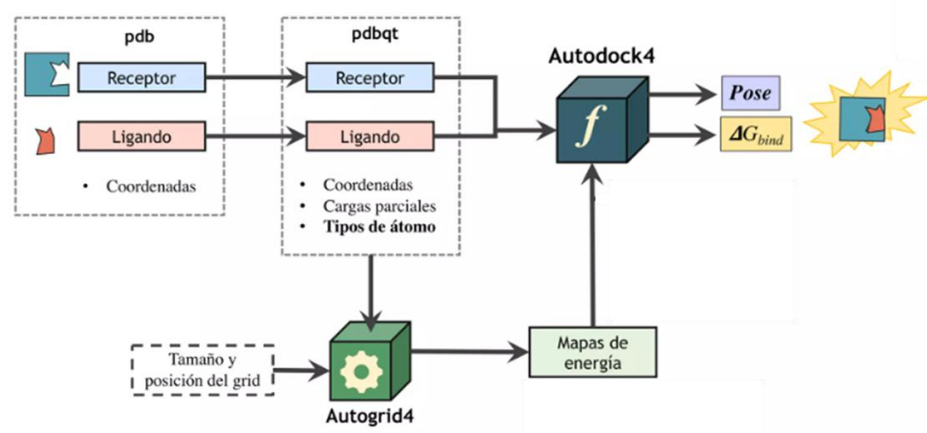
\includegraphics[width = 0.7\textwidth]{figs/docking-pipeline.png}
\end{figure}

\section{Práctica}
El ligando es el fichero jnj.pdb, y la proteína es P2X7-SWISSMODEL.pdb. Con esto localizado, vamos al programa Avogadro. Al descargar un ligando o fármaco, no es real, es plano. Por ello, Avogadro permite minimizar la estructura a una más real. 

Al final hemos utilizado la tolcapona. En PubChem hemos buscado tolcapone y descargado la estructura 3D en SDF. Esto lo abrimos en Avogadro. En la barra superior hay un botón con una E y una flecha hacia abajo (tres botones a la izquierda de Tool Settings). Seleccionamos el campo de fuerza MMFF94 con 4 pasos por update y pulsamos start. 

\begin{figure}[h]
\centering
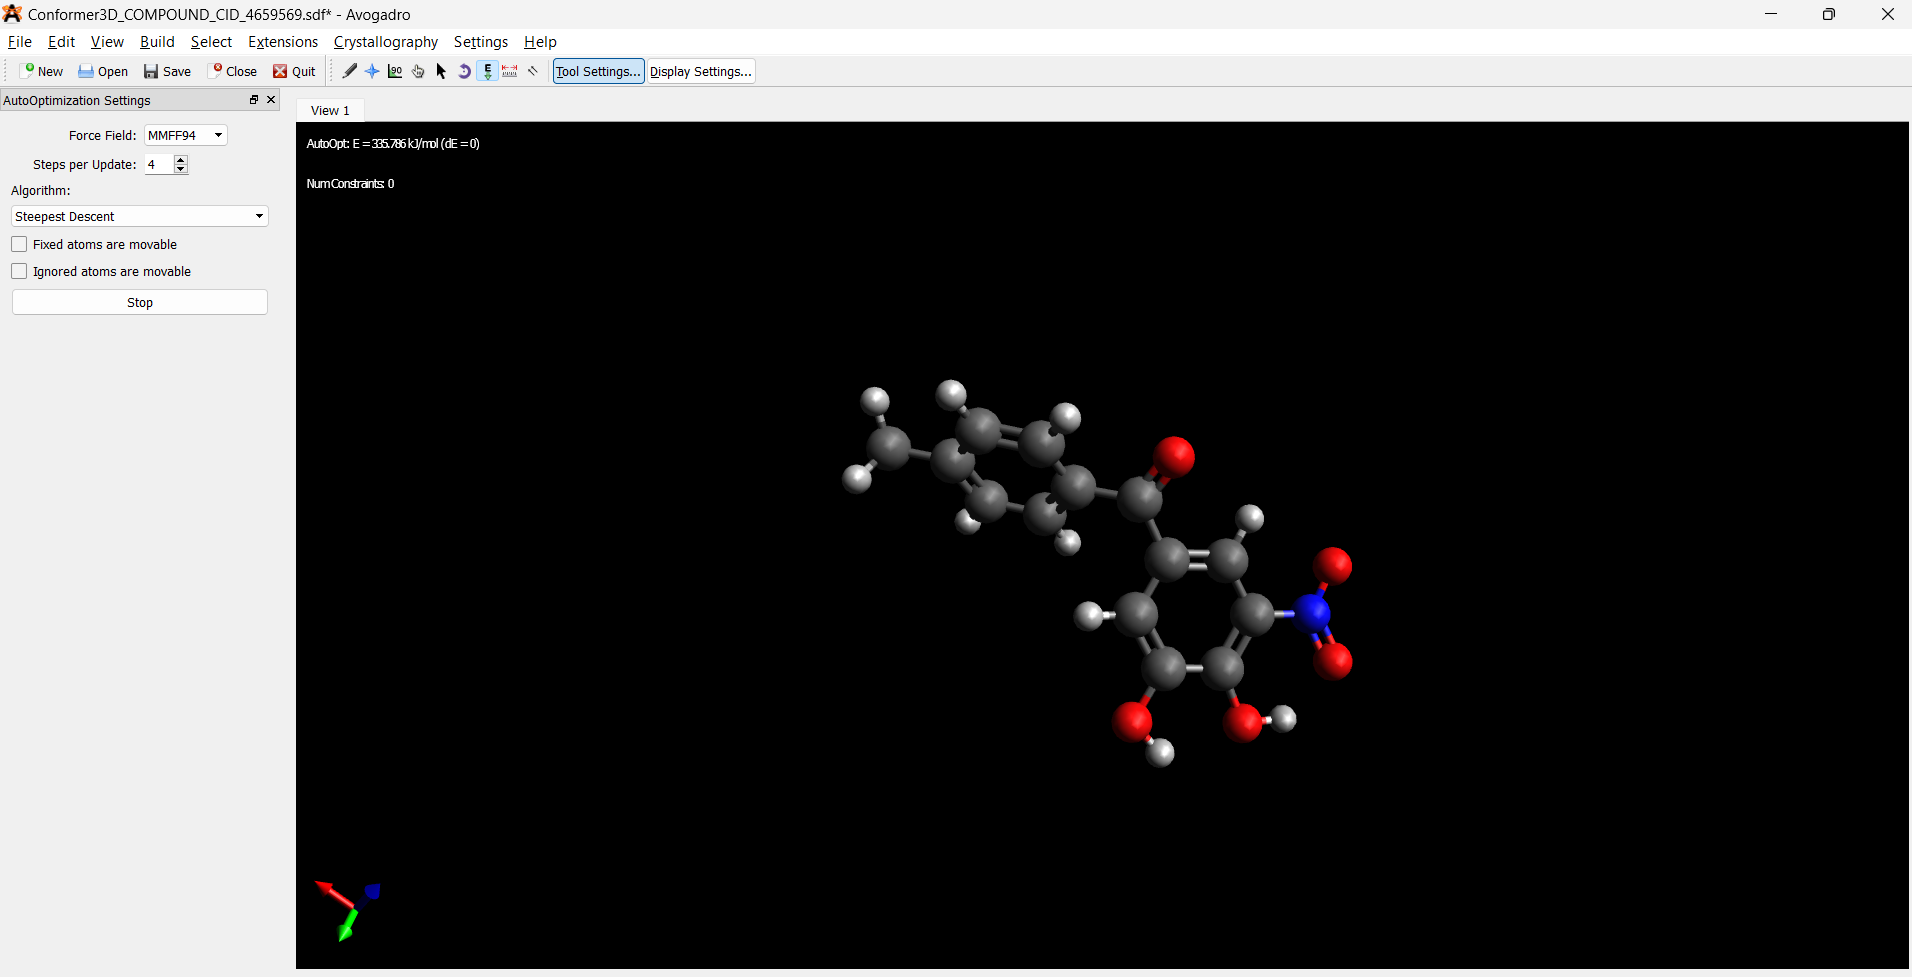
\includegraphics[width = 0.7\textwidth]{figs/avogadro-tolcapona.png}
\end{figure}

Una vez terminado, lo guardamos en formato PDB y abrimos Chimera. Ahí abrimos P2X7-Swissmodel.pdb. A continuación vamos a Tools > Surface/Binding Analysis > Dock Prep. Es importante que esté marcada la opción de "Add hydrogens" y "Add charges". Este programa trabaja con estructuras en formato Mol2 para docking, por lo que esa opción también debe estar habilitada. En la siguiente pantalla debe considerar todos los enlaces de hidrógeno. Como la histidina es el aminoácido más complejo de protonar in silico, se especifica (lo dejamos por defecto, pero en estudios in silico es importante revisarlo). En cuanto a las cargas, utilizamos los residuos estándar AMBER ff14SB. La siguiente pestaña es para guardar el archivo. Le ponemos un nombre (que en este caso es p2x7\_dockprep) y lo guardamos.

En una nueva sesión abrimos jnj y volvemos a ir a Dock Prep. Repetimos lo mismo, pero en el campo de fuerzas cambiamos AM1-BCC por Gasteiger. Vemos que la carga neta es +1 y volvemos a asegurarnos de que el método sea Gasteiger. Guardamos el ligando en formato mol2. 

Cerramos la sesión y abrimos los dos ficheros .mol2 que acabamos de generar. Debemos alejarnos, ya que las dos estructuras no están juntas. Habiendo leído bibliografía previa, sabemos que el ligando se une a la proteína en la zona de beta láminas y no en las hélices alfa. Nos interesa que el ligando se una en el centro del poro o en alguna zona lateral. Ahora vamos a Favorite > Model Panel y se desmarca la proteína para poder mover el ligando. Ahora lo podemos colocar cerca del poro. Una vez terminado, Tools > Surface/Binding Analysis > Autodock Vina > Browse y ponemos un nombre de fichero. Después de aceptar seleccionamos como receptor la proteína y ligando nuestro ligando. En Receptor search volume options ponemos un 10 en todas las filas para que aparezca la caja en cualquier sitio. Al pulsar la ruedecita del centro del ratón, se selecciona toda la proteína directamente. También podemos mover la caja independientemente y ajustarla manualmente. Idealmente, la parte de las hélices alfa está fuera. Si siempre trabajamos con la misma proteína, conviene apuntarnos las coordenadas buenas que se han actualizado en el panel anterior. En opciones de receptor deben estar todos en verdadero salvo "ignore all non-standard residues", que debe estar en falso. El resto lo dejamos por defecto salvo Number of Binding Models, que lo subimos a 10. En executable location, debemos asegurarnos de que esté el path del ejecutable (que suele estar en C:/Program Files(x86)/The Scripp Research Institute/Vina/vina.exe).

\begin{figure}[h]
\centering
\includegraphics[width = 0.7\textwidth]{figs/docking.png}
\end{figure}

Una vez terminado, aparece una tabla con las distintas uniones ordenadas. Las interacciones deberían estar a no más de 5 $\AA$ y se debe revisar manualmente que el docking es real y no esté en mitad de la proteína. Se puede mirar en PyMOL abriendo los ficheros docking.pdbqt y docking.receptor.pdbqt. 
%07/03 - Myriam
\chapter{Dinámica molecular}
\section{Conceptos teóricos}
La dinámica molecular es la simulación informática en la que átomos y moléculas interactúan durante un periodo de tiempo y los movimientos de las distintas partículas pueden visualizarse a posteriori. No tiene en cuenta los movimientos de los electrones, considerando la energía de las moléculas en función de los movimientos de sus núcleos, siendo así ideal para macromoléculas. La mecánica clásica se basa en las leyes de Newton. Las ecuaciones de movimiento se resuelven para predecir las posiciones y velocidades de los átomos en cada paso temporal.

La aproximación de Born-Oppenheimer dice que la energía de una molécula en su estado basal puede considerarse como una función de las coordenadas de los núcleos atómicos. Los campos de fuerza permiten calcular las fuerzas de los átomos. Algunos ejemplos de campos de fuerza que se usan son GAFF, AMBER y CHARMM.

Los pasos de una dinámica molecular son:
\begin{enumerate}
\item Preparación del sistema: se hace a partir de fuentes experimental o teóricas. La parametrización incluye cargas formales, adaptación del ligando y la proteína, etc. A continuación el sistema se mete en una caja de agua. La idea es que se simula un sistema con condiciones fisiológicas como si fuera un experimento real.
\item Minimización: consiste en minimizar el complejo y la caja de agua. Hace referencia a que el sistema esté estable y en equilibrio.
\item Calentamiento: se pueden tener varias etapas de calentamiento con un máximo de 300 K. Si hay varias, se pueden hacer de forma progresiva. En los artículos que utilicen dinámica molecular, suelen indicar las condiciones (temperatura, presión, duración de la dinámica, etc.)
\item Equilibrado: se trabaja en condiciones normales con presión de 1 atmósfera generalmente, pero hay que ajustarlo siempre.
\item Producción: es la etapa de dinámica molecular, el paso importante. Si todo ha ido bien en los pasos anteriores, no debería haber problemas, mientras que si algo falla, se deben añadir restricciones u otros parámetros. Aquí es donde realmente se establece la duración de la dinámica. Cuanto mayor duración, más espacio explorable tiene la molécula y mayor tiempo de cálculo se necesita. La producción produce la trayectoria.
\end{enumerate}

La dinámica molecular se utiliza para:
\begin{itemize}
\item Se estudian procesos como la apertura y cierre de canales iónicos, cambios en la estructura de proteínas reguladoras...
\item Estudio de la estabilidad de los complejos
\item Se analizan las posibles rutas de plegamiento y se identifican estados intermedios metaestables. 
\item Estudio de la cinética del crecimiento de cristales en soluciones y su relación con la estabilidad de los fármacos.
\item La interacción de las moléculas con la bicapa lipídica se estudia para comprender su permeabilidad y absorción en los sistemas biológicos.
\end{itemize}

Después de la dinámica molecular se suelen hacer algunos \textbf{análisis de estabilidad}:
\begin{itemize}
\item \textbf{RMSD}: Evaluación de los cambios conformacionales de una molécula o complejo a lo largo del tiempo. Se debe comprobar que no haya muchos picos marcados.
\item \textbf{RMSF}: Medición de la fluctuación media de cada residuo de proteína durante la simulación 
\end{itemize}

Con DiscoveryStudio y PyMOL se pueden realizar análisis de interacciones, marcando los aminoácidos que han interaccionado con el ligando.

Los cálculos de MMPBSA/GBSA resuelve una ecuación termodinámica para obtener una tabla que recoja los aminoácidos más importantes que interaccionan. Es como un docking más preciso al desglosar la tabla de energía en las distintas interacciones (polares, a polares, electroestáticas, van der Waals, etc.).

\section{Práctica}
Abrimos VMD. Nos famos a File, New molecule, Load file y primero cargamos step5\_input.parm7. Así cargamos las coordenadas. En la misma pestaña de Molecule File Browser hay que cargar el fichero short\_orai1.mdcrd con file type AMBER Coordinates with Periodic Box. Le damos a load y aparece el cuadrado con la caja de agua. 

Ahora vamos a Graphics > Representation y podemos escribir lo que queremos ver. Si vamos a Selections, se sugieren frases o condiciones de lo que se quiere ver. Por ejemplo, podemos poner "all and not waters" para visualizar solo la membrana lipídica con el poro. En lugar de darle a Apply, se le puede dar a Create Rep para guardar ambas representaciones. 

\begin{figure}[h]
\centering
\includegraphics[width = 0.5\textwidth]{figs/lipid-rep.png}
\end{figure}

\newpage

Ahora repetimos lo mismo con el documento complex-vilazodone-p2x7.top y seleccionamos AMBER7 Parm como tipo. Cargamos y seleccionamos el short con la caja de agua. En representación, ponemos all with not waters. 

\begin{figure}[h]
\centering
\includegraphics[width = 0.4\textwidth]{figs/protein-dynamics.png}
\end{figure}

Ponemos crear una representación con all and not waters and not protein para ver el ligando y cómo se mueve con las distintas conformaciones. 

En la pestaña principal, podemos dar click derecho y guardar las coordenadas. Se genera un documento pdb en el que está la tabla.

\begin{figure}[h]
\centering
\includegraphics[width = 0.7\textwidth]{figs/md-tabla.png}
\end{figure}

Ahora abrimos Discovery Studio y abrimos el documento complex\_orai1\_telmisartan. Este contiene la proteína. Abrimos el documento de complex\_telmisartan y tenemos el ligando. Pulsamos con click derecho en el ligando y seleccionamos Custom Carbon atoms only y ponemos un color azul. De la misma forma lo copiamos y pegamos con la proteína. Ahora debemos seleccionar solo el ligando e ir a Receptor-Ligand Interaction > Ligand Interactions. En Interaction Options desseleccionamos Show Intramolecular interactions en la parte de abajo. Con click derecho se pueden añadir etiquetas, y se puede mostrar un diagrama 2D de las interacciones y sus tipos.

\begin{figure}[h]
\centering
\includegraphics[width = 0.7\textwidth]{figs/2d-diagram-docking.png}
\end{figure}

Volvemos a abrir el fichero con la proteína sola. En la parte izquierda nos vamos a Define and Edit Binding Site y From Receptor Cavities. Al lado del panel hay una flechita que podemos expandir. Ahí sale una lista con los posibles sitios de unión. 

\begin{figure}[h]
\centering
\includegraphics[width = 0.7\textwidth]{figs/binding-sites.png}
\end{figure}

Copiamos el fichero docking.pdbqt para duplicarlo. Lo llamamos lig1 para quedarnos solo con el primer modelo. Aprovechamos también para limpiar el fichero. Eliminamos todos los modelos que no sean el 1, eliminamos la cabecera, eliminamos todos los ROOT, BRANCH, ENDBRANCH y demás, y al final también eliminamos todo. Nos debemos quedar sólo con HETATM, y tras la última fila añadimos TER y END. Discovery Studio no reconoce los ficheros PDBQT de Docking, por lo que podemos abrirlos en PyMOL, ir a Export Molecule y exportarlo a PDB.

\end{document}
